\documentclass[11pt]{article}
\usepackage[T1]{fontenc}
\usepackage{lmodern}
\input{glyphtounicode}
\input{glyphtounicode-cmex}
\pdfgentounicode=1
\usepackage[margin=1in]{geometry}
\usepackage{amsmath,amssymb,amsthm,mathtools}
\usepackage{microtype}
\usepackage{booktabs,array,enumitem}
\usepackage{float}
\usepackage{tikz}
\usetikzlibrary{arrows.meta,calc,patterns,positioning}
\usepackage[colorlinks=true,linkcolor=blue!55!black,citecolor=blue!55!black,urlcolor=blue!55!black]{hyperref}
\pdfinfoomitdate=1
\pdftrailerid{}
\pdfsuppressptexinfo=15
\setlength{\emergencystretch}{2em}
\numberwithin{equation}{section}
\newtheorem{theorem}{Theorem}[section]
\newtheorem{lemma}[theorem]{Lemma}
\newtheorem{proposition}[theorem]{Proposition}
\newtheorem{corollary}[theorem]{Corollary}
\theoremstyle{definition}
\newtheorem{definition}[theorem]{Definition}
\theoremstyle{remark}
\newtheorem{remark}[theorem]{Remark}
\DeclareMathOperator{\Tr}{Tr}
\DeclareMathOperator{\id}{id}
\DeclareMathOperator{\supp}{supp}
\DeclareMathOperator{\dist}{dist}
\DeclareMathOperator{\diam}{diam}
\DeclareMathOperator{\Sym}{Sym}
\DeclareMathOperator{\poly}{poly}
\newcommand{\E}{\mathbb E}
\newcommand{\R}{\mathbb R}
\newcommand{\C}{\mathbb C}
\newcommand{\Z}{\mathbb Z}
\newcommand{\N}{\mathbb N}
\newcommand{\ket}[1]{\lvert #1\rangle}
\newcommand{\bra}[1]{\langle #1\rvert}
\newcommand{\norm}[1]{\lVert #1\rVert}
\title{A two-dimensional area law from a global spectral gap}
\author{OpenAI}
\date{September 24, 2026}
\hypersetup{pdftitle={A two-dimensional area law from a global spectral gap},
            pdfauthor={OpenAI}}
\begin{document}
\maketitle
\begin{abstract}
We prove an entropy area law for the unique ground state of a finite-range
Hamiltonian on any finite induced subgraph of the square lattice. A lower bound
on the spectral gap of the full Hamiltonian and fixed bounds on the local
dimension, interaction range, and interaction strength suffice. For every set
of sites, its entanglement entropy is bounded by a constant times the number of
edges crossing its boundary, independently of the size and shape of the domain.
\end{abstract}
\tableofcontents
\clearpage
\section{Introduction}\label{sec:introduction}

The entanglement entropy of a pure quantum state measures how much information
is shared by a region and its complement. Its elementary upper bound is
proportional to the number of sites in the region. An area law replaces this
volume by the number of interactions crossing the region's boundary. We prove
such a bound for the unique gapped ground state of a general finite-range
Hamiltonian in two dimensions.

\subsection{The setting and the theorem}

Let $\Lambda\subset\Z^2$ be finite. Its edges join pairs at Euclidean distance
one, so that $\Lambda$ carries the induced square-lattice graph. Write
$d_\Lambda$ for graph distance, with value $+\infty$ between different
components. At each site put a copy of $\C^q$, and write
$\mathcal H_\Lambda=\bigotimes_{x\in\Lambda}\C^q$.
An operator supported on $X\subseteq\Lambda$ acts as the identity on the other
tensor factors. An admissible Hamiltonian has the form
\begin{equation}\label{eq:hamiltonian}
 H=\sum_{\substack{\varnothing\ne X\subseteq\Lambda\\
                  \diam_{d_\Lambda}X\le R}}h_X,
 \qquad h_X=h_X^*,\qquad \norm{h_X}\le J.
\end{equation}
There is one summand for each support $X$; a summand may be zero.
Here $q\ge1$ and $R\ge0$ are fixed integers and $J>0$ is fixed.
This indexing convention bounds the sum of interaction norms at every site
in terms of $R,J$ alone.

For $A\subseteq\Lambda$ define the edge boundary
\[
 \partial_\Lambda A=
 \{\{x,y\}:x\in A,\ y\in\Lambda\setminus A,\ |x-y|_1=1\}.
\]
If $\Omega\in\mathcal H_\Lambda$ is a unit vector, write
$\rho_A=\Tr_{\Lambda\setminus A}\ket{\Omega}\bra{\Omega}$ and
$S_\Omega(A)=-\Tr\rho_A\log\rho_A$, with $0\log0=0$.
All logarithms are natural.

\begin{theorem}[Area law]\label{thm:area}
For every $q,R,J$ as above and every $\Delta>0$, there is a finite constant
$C=C(q,R,J,\Delta)$ with the following property. Suppose that $\Lambda$ is a
finite induced square-lattice domain and that the Hamiltonian
\eqref{eq:hamiltonian} has a unique normalized ground vector $\Omega$, up to
phase, with ground energy $E_0$, and satisfies
\[
 H-E_0\id\ \ge\ \Delta\bigl(\id-\ket{\Omega}\bra{\Omega}\bigr).
\]
Then for every $A\subseteq\Lambda$,
\begin{equation}\label{eq:area-law}
 S_\Omega(A)\le C\,|\partial_\Lambda A|.
\end{equation}
The same constant applies to all such domains, sets, and Hamiltonians.
\end{theorem}

The distance in \eqref{eq:hamiltonian} is the distance within the induced
graph. This distinction matters for domains with holes or disconnected
components. The spectral assumption concerns the full Hamiltonian; no gap
assumption is imposed on Hamiltonians restricted to smaller regions.

For completeness, the theorem also gives the usual vertex-boundary
formulations. Define
\[
 \partial_{\rm in}A=\{x\in A:\exists y\notin A,
                \ \{x,y\}\in\partial_\Lambda A\},
 \qquad
 Z_A=\bigcup_{e\in\partial_\Lambda A}e.
\]

\begin{corollary}\label{cor:rectangles}
The conclusion of Theorem~\ref{thm:area} holds for every subset of a finite
rectangular square lattice with bounded on-site and nearest-neighbor
interactions and a unique ground state separated by a fixed global gap.
For every domain covered by that theorem it also implies
\[
 S_\Omega(A)\le4C|\partial_{\rm in}A|,
 \qquad S_\Omega(A)\le2C|Z_A|.
\]
\end{corollary}
\begin{proof}
On-site and nearest-neighbor interactions have graph range at most one.
Each inner boundary vertex is incident with between one and four crossing
edges, so $|\partial_{\rm in}A|\le|\partial_\Lambda A|
\le4|\partial_{\rm in}A|$. Counting both endpoints gives
$|Z_A|\le2|\partial_\Lambda A|\le4|Z_A|$.
These inequalities include empty boundaries.
\end{proof}

\subsection{History and related work}
The relation between entanglement and boundary area arose in quantum-field
calculations motivated by black-hole entropy.  Bombelli, Koul, Lee, and
Sorkin related entropy from tracing inaccessible quantum-field degrees of
freedom to black-hole area~\cite{BombelliEtAl1986}; Srednicki subsequently found area scaling
numerically for a spherical region in the vacuum of a regulated free
massless scalar field~\cite{Srednicki1993}.  These calculations motivated
the entanglement area-law question through regulated field models. For
finite-dimensional lattice spins, the gap-to-area conjecture asks whether
a unique ground state has an entropy bound proportional to boundary area
when local dimension, interaction range and strength are bounded and the
spectral gap has a size-independent positive lower
bound~\cite{Hastings2007,AradLandauVazirani2012}.
Theorem~\ref{thm:area} gives an affirmative answer in the stated
two-dimensional induced-domain setting.

In one dimension, Hastings proved a length-independent entropy bound for
the unique ground state of a finite-range Hamiltonian with uniformly
bounded interactions, fixed local dimension, and a positive spectral
gap~\cite{Hastings2007}.  Arad, Landau, and Vazirani improved the dependence
on the inverse gap for frustration-free chains using approximate ground-state
projectors~\cite{AradLandauVazirani2012}.  These are operators that preserve
the ground vector while contracting its orthogonal complement, with
controlled growth of Schmidt rank.  Arad, Kitaev, Landau, and Vazirani
extended this approach to general, possibly frustrated
chains~\cite{AradKitaevLandauVazirani2013}.  A complementary result of Brand\~ao and Horodecki
derives an area law for pure one-dimensional states from exponential
decay of correlations between arbitrary separated
regions~\cite{BrandaoHorodecki2015}.  This region-wise hypothesis is
stronger than decay of single-site correlation functions.  More generally,
the exponential clustering theorem relates a spectral gap to decay of
connected correlations of separated
observables~\cite{NachtergaeleSims2006}; an entropy estimate requires
control of the reduced state's full spectrum.
Anshu, Harrow, and Soleimanifar obtained boundary-dependent bounds on
smooth entanglement spread, which measures the width of the significant
part of that spectrum, including square-root boundary scaling on lattices
up to logarithmic factors~\cite{AnshuHarrowSoleimanifar2022}.  Such a width
estimate leaves the location of the spectrum, and hence its entropy,
to be controlled.

Strict area-law bounds in higher dimensions are also known for
restricted model classes.  Cramer, Eisert, Plenio, and Drei\ss ig proved
such a bound for arbitrary regions in cubic harmonic lattices with a
finite-range positive potential matrix whose condition number is
uniformly bounded~\cite{CramerEisertPlenioDreissig2006}.  These Gaussian
models have infinite-dimensional oscillator sites and provide a
comparison with the finite-dimensional spin setting considered here.

Other higher-dimensional results make additional spectral or thermodynamic
assumptions.  Masanes obtained bounds with logarithmic corrections from correlation
decay and bounds on the number of low-energy states of restricted
Hamiltonians~\cite{Masanes2009}; Brand\~ao and Cramer obtained a logarithmically
corrected bound for cubic regions under a low-temperature heat-capacity
hypothesis~\cite{BrandaoCramer2015}.  Cho proved strict area scaling for
balls along boundary-growth families satisfying uniform gaps and an
additional compatibility condition on successive reduced ground
states~\cite{Cho2014}.  These conditions supply information beyond the gap
of the single full Hamiltonian considered here.

For two-dimensional spin systems, Anshu, Arad, and Gosset proved a
subvolume bound for rectangular regions in a rectangular lattice with
plaquette projector interactions, a unique frustration-free ground
state, and a uniform local gap~\cite{AnshuAradGosset2022Subvolume}.
At fixed local dimension and local gap, the bound is
\(O(b^{5/3}\log^{7/3}(2+b))\), where \(b\) is the rectangle's boundary
size.  Their subsequent result gives
\[
  S\le n^{\,1+O((\log n)^{-1/5})}
\]
across a vertical cut of length \(n\), again for locally gapped,
frustration-free plaquette projector models with a unique ground
state~\cite{AnshuAradGosset2022Area}.  The local-gap assumption concerns
restrictions of the Hamiltonian; it is stronger than a gap for the full
system alone.  The latter entropy bound is near-linear, and its theorem
concerns vertical cuts.  The setting considered here allows frustrated
interactions, assumes a gap only for the full Hamiltonian, and includes
arbitrary regions in arbitrary finite induced square-lattice domains.
Arad, Firanko, and Jain extend approximate-projector methods to
maximally mixed ground states and bound their mutual information, with a
two-dimensional application under frustration-free and local-gap
assumptions~\cite{AradFirankoJain2026}.

The proof below combines locality estimates with ways of expressing entropy
through operator norms. For locality, we use the Lieb--Robinson
framework~\cite{LiebRobinson1972,NachtergaeleOgataSims2006} and Kitaev's
centered spectral filter~\cite[Appendix~D.1.2]{Kitaev2006Anyons}.
Swingle and McGreevy discuss positive constraints obtained by squaring
filtered terms, for which retaining a gap is a separate
issue~\cite[Section~8.4]{SwingleMcGreevy2016}. Here taking absolute
values gives the operator domination that retains the full-system gap.
Later, products of positive contractions derived from these constraints
preserve the ground state and suppress excitations, as projection products
do in detectability-lemma arguments~\cite{AnshuAradVidick2016}. Their localization uses propagation
estimates for unital channels, related to dissipative Lieb--Robinson
bounds~\cite{BarthelKliesch2012}; the coupled random-product estimate
needed here is proved in Section~\ref{sec:amplification}.

For the entropy comparison, bounds on local entanglement production are a
precedent for controlling logarithmic commutators independently of
spectator dimensions~\cite{VanAcoleyenMarienVerstraete2013}.
Section~\ref{sec:initial} proves the quadratic real-part estimate needed
for our marginal tails. Strong subadditivity and conditional-entropy
continuity supply the entropy inequalities used throughout
\cite{LiebRuskai1973,AlickiFannes2004,Winter2016}.
We encode marginal spectra on symmetric tensor powers using
Schur--Weyl duality~\cite{EtingofEtAl2011}, whose connection with spectrum
estimation is developed by Keyl and Werner~\cite{KeylWerner2001}.
The passage back to one-copy vectors uses finite quantum de~Finetti
measures~\cite{ChristandlEtAl2007,LewinNamRougerie2015} and the product
calculus of symmetrized finite observables~\cite{RaggioWerner1989}.
Weighted operator geometric means~\cite{PuszWoronowicz1975,KuboAndo1980}
combine the changing partitions, while the modular comparison starts
from the resolvent-compression identity of Carlen and
Vershynina~\cite[Lemma~2.1]{CarlenVershynina2019}.
The detailed construction uses these ingredients to compare entropy gain
and excitation energy in the same family of states; the next overview
explains how that comparison leads to the area bound.


\subsection{A tensor-network consequence}

A projected entangled-pair state (PEPS) is specified by one tensor at each
lattice site, with a physical index for that site's state and one virtual
index for each incident edge. Contracting the paired virtual indices gives
a many-body vector. The dimension of an edge index is its bond dimension.
The approximation problem asks how large these dimensions must be to
approximate the ground vector on the original lattice.

The companion \cite[Theorem~1.1]{OpenAI2026PolynomialPEPS} proves a
polynomial bound for the original open $L\times L$ square grid, $L\ge2$,
with on-site and nearest-neighbor interactions. For fixed local dimension
$q\ge2$, term-norm bound $J>0$, and global gap $\Delta>0$, every unique
ground vector in this class has a PEPS approximation with maximum bond
dimension at most $CL^c$ and global vector error at most $L^{-1}$ after
normalization and phase choice. The constants depend only on $q,J,\Delta$.
This is an existence result; it does not assert an efficient tensor
construction or contraction algorithm.

The approximation uses more than the entropy inequality. This paper also
provides positive operators that annihilate the ground vector and have
rapidly decaying spatial tails (Proposition~\ref{prop:positive}),
quantitative information bounds across collars
(Propositions~\ref{prop:collar} and \ref{prop:amplification}), and
two families of geometrically separated regions
(Proposition~\ref{prop:two-families}), with the region shapes and clearances
specified in those results. The companion combines these estimates and the
geometric ordering with additional compression and routing arguments;
its PEPS result is a consequence of that further analysis.

\subsection{How the proof is organized}

Fix the set $A$ whose entropy is to be bounded, and let $Z_A$ be its
crossing-edge endpoints. For disjoint physical regions $B,C$, write
\[
 I_\Omega(B:C)=S_\Omega(B)+S_\Omega(C)-S_\Omega(B\cup C)
\]
for their mutual information. Our analytic goal is to make this quantity
small when $B$ lies inside $A$ and $C$ is beyond a suitable collar,
even when $C$ includes all of $\Lambda\setminus A$.
Here is why this suffices. Suppose that, after removing a set $D$ of
$O(|\partial_\Lambda A|)$ sites, we can partition $A$ into two ordered
families of regions. If each region shares little information with the
complement of $A$ together with the earlier regions of its own family,
two applications of the entropy chain rule cancel all individual region
entropies. Purity then bounds $S_\Omega(A)$ by $|D|\log q$ and the sum
of the information errors. Section~\ref{sec:geometry} constructs regions
with the required ordering and separation.

The analytic estimates concern intersections of $A$ with ambient boxes or
finite unions of rectangles and triangles. Their clearance is from $Z_A$;
they may meet holes or the edge of the physical domain. Hamiltonian
locality and propagation always use neighborhoods in the induced graph.
The argument has five stages.
\begin{enumerate}[leftmargin=*,label=\arabic*.]
\item \emph{Obtain a first exponent below volume.}
Section~\ref{sec:initial} uses the global gap to bound fluctuations of the
negative logarithms of positive marginal eigenvalues. It then optimizes
products of positive operators on nested rectangles. Two bounds on the
optimized norm, one using the energy estimate and global gap, give a
conditional-entropy discount, and hence
\[
 S_\Omega(A\cap Q)\le Cr^{1+e_0},\qquad e_0<1,
\]
for a box $Q$ of side at most $r$ sufficiently far from $Z_A$.

\item \emph{Control information and energy in the same interpolation.}
Section~\ref{sec:quasilocal} replaces the Hamiltonian by a sum of positive
operators that annihilate $\Omega$ separately, retain a global gap, and
have rapidly decaying graph-local tails.
Sections~\ref{sec:conditional}--\ref{sec:transport} associate positive
operators to partitions of the full system and interpolate between them
as a small subsystem changes parts. These operators act on symmetric
tensor powers, whose vectors are fixed by every permutation of the copies.
Applying an inverse power of the interpolating operator to a vector built
from ground-state copies and an auxiliary entangled pair defines the
filtered vector whose norm we study. As the copy number grows, logarithmic
norms per copy can be compared with combinations of marginal entropies.
The decrease of a suitable logarithmic squared norm is bounded below by averaged conditional mutual
information, up to a small error. The same transported states bound the
energy cost. This common control permits a comparison of information
gained with excitation energy spent.

\item \emph{Compare the norms and scan a collar.}
Section~\ref{sec:comparators} gives two bounds on the negative logarithm
of the filtered vector's norm. Auxiliary dimensions are chosen from a
high-probability part of the target's Schmidt spectrum. Projecting the
target and an auxiliary system onto an entangled pair gives the upper
bound. The lower bound uses the global gap: low physical energy forces
most copies into the ground state.
Section~\ref{sec:scanner} moves the partitions through a collar according
to a finite randomized schedule. Each interaction is rarely split by a
moving boundary, and the schedule supplies an interpolation with sufficiently
low energy. The two norm bounds first improve the box exponent repeatedly;
their sharper form then gives
\[
 I_\Omega(A\cap T:\Lambda\setminus(A\cap T_L))
       \le Cn^{1-\varepsilon}.
\]
Here $T$ is one of the finite unions of controlled rectangles and triangles
specified in Definition~\ref{scanner:template}, $\varepsilon>0$ is fixed,
and $T_L$ is the ambient sup-norm enlargement by
$L=\lfloor n^{1-\varepsilon}\rfloor$. These targets and their allowed
enlargements have $O(n)$ boundary edges. The entire finite physical and
auxiliary system and schedule are fixed before the copy number tends to infinity.

\item \emph{Amplify the information bound.}
Section~\ref{sec:amplification} uses typical spectral subspaces to
construct a candidate operator for restoring a target moved to an auxiliary
reference. Its norm is controlled by the collar information. A localized
product of contractions derived from the positive constraints suppresses
the excited component, and polar decomposition yields a unitary comparison near the target. This unitary
leaves both the reference and the remote physical system untouched;
comparison with a state in which they are independent bounds their
original mutual information. Enlarging the collar by a sublinear radius
makes the bound smaller than any prescribed inverse power of $n$.

\item \emph{Arrange the regions for entropy cancellation.}
Section~\ref{sec:geometry} builds the two ordered families described above.
The collar around each region avoids the complement of $A$ and all earlier
regions of its own family. Narrow strips and recursive repairs at point
contacts produce these separations for arbitrary cuts while leaving only
$O(|\partial_\Lambda A|)$ sites uncovered. The information errors are
summable over the regions, so the two entropy chains prove
\eqref{eq:area-law}.
\end{enumerate}

\section{Entropy and induced-graph locality}\label{sec:prelim}

We record the finite-dimensional conventions and elementary uniform bounds
used throughout the proof. Unless specified otherwise, entropies refer to the
original ground vector $\Omega$. A changed state is shown by a subscript.
Juxtaposition of disjoint systems denotes their tensor product or their union.

\subsection{Entropy identities and continuity}

For a density matrix $\rho$ on systems $D,E,F$, define
\[
 S(D|E)_\rho=S(DE)_\rho-S(E)_\rho,
 \quad I(D:E)_\rho=S(D)_\rho+S(E)_\rho-S(DE)_\rho,
\]
and
\[
 I(D:F|E)_\rho=S(DE)_\rho+S(EF)_\rho-S(E)_\rho-S(DEF)_\rho.
\]
We use strong subadditivity, $I(D:F|E)_\rho\ge0$, for normalized
finite-dimensional density operators~\cite{LiebRuskai1973}.
It implies that conditioning decreases conditional entropy and that discarding
systems cannot increase mutual information. Subadditivity and purification
give $|S(D|E)|\le\log\dim D$. For a pure state the entropies of complementary
systems coincide. These facts also hold with empty regions, whose
Hilbert spaces are the one-dimensional empty tensor product.

Write $h(u)=-u\log u-(1-u)\log(1-u)$ for binary entropy.
The trace distance of two states is half the trace norm of their difference.
The continuity estimate below uses the dimension-independent conditional
entropy method of Alicki and Fannes~\cite{AlickiFannes2004}, in Winter's
sharpened form~\cite{Winter2016}.

\begin{lemma}[Continuity with a fixed controlled system]\label{lem:continuity}
Let $\rho,\sigma$ be density operators on finite-dimensional $D\otimes E$,
and put $\delta=\tfrac12\norm{\rho-\sigma}_1\le1$ and $d_D=\dim D$.
Then
\begin{equation}\label{eq:conditional-continuity}
 |S(D|E)_\rho-S(D|E)_\sigma|
 \le2\delta\log d_D+(1+\delta)
                 h\left(\frac{\delta}{1+\delta}\right)
 \le C\sqrt\delta\log(e d_D).
\end{equation}
The same estimates hold for $S(D)$ by making $E$ trivial. Summing the
bounds for $S(D)$ and $S(D|E)$ therefore bounds the continuity cost for
$I(D:E)$ in terms of $d_D$, independently of $\dim E$.
\end{lemma}
\begin{proof}
We include the mixture argument for the bound in
\cite[Lemma~2]{Winter2016}. If $\tau=\sum_j p_j\tau_j$, adding a classical
register that records $j$ shows
\[
 0\le S(D|E)_\tau-\sum_jp_jS(D|E)_{\tau_j}\le H(p).
\]
For the lower bound, condition on that register and use strong
subadditivity. For the upper bound, use the ordinary mixing upper bound on
$S(DE)$ and concavity of $S(E)$. The ordinary bound follows by recording a
duplicate of the classical register: its conditional entropy given $DE$
is nonnegative after this further conditioning.

If $\delta>0$, write the Jordan decomposition
$\rho-\sigma=\delta(\tau_+-\tau_-)$, where $\tau_\pm$ are states.
Then
\[
 \frac{\rho+\delta\tau_-}{1+\delta}
 =\frac{\sigma+\delta\tau_+}{1+\delta}.
\]
Apply the mixture bounds to both expressions and use
$|S(D|E)_{\tau_+}-S(D|E)_{\tau_-}|\le2\log d_D$.
This proves the first inequality. The second follows from the elementary
bound $h(u)\le C\sqrt u$. The case $\delta=0$ is immediate.
Finally, $I(D:E)=S(D)-S(D|E)$, so the two displayed entropy bounds apply.
\end{proof}

The trace distance between pure states represented by unit vectors $\xi,\eta$
is at most $\norm{\xi-\eta}$. We will use Lemma~\ref{lem:continuity} on
regions with a controlled number of sites, or with the controlled region as
the first argument of a conditional entropy. In this way estimates never
acquire the dimension of an uncontrolled complement.

\subsection{Local counting and degenerate cases}

For a site $x$ let $B_\Lambda(x,r)=\{y:d_\Lambda(x,y)\le r\}$.
A path of length $r$ has ambient $\ell^1$ displacement at most $r$; hence,
for an integer $r\ge0$,
\begin{equation}\label{eq:ball-count}
 |B_\Lambda(x,r)|\le v_r:=1+2r(r+1).
\end{equation}
For a physical set $D$ put
$N_r^\Lambda(D)=\{x:d_\Lambda(x,D)\le r\}$.
We reserve graph neighborhoods for support and propagation estimates.
An ambient dilation of a finite set $T\subset\Z^2$ is instead
$T_j=T+([-j,j]^2\cap\Z^2)$ for integer $j\ge0$.

Assign each nonzero interaction in \eqref{eq:hamiltonian} an anchor in its
support. The number of terms containing any prescribed site is at most
\[
 \mu_R:=2^{v_R-1},
\]
because each such support is a subset of its radius-$R$ graph ball containing
that site. In particular, the number of anchored terms at a site is at most
$\mu_R$, and the sum of norms of terms containing that site is at most
$J\mu_R$. Terms with scalar identity factors still obey these bounds with
their assigned supports.

Call an assigned support \emph{split} by a set $D$ when it meets both $D$ and
$\Lambda\setminus D$. For a split support, a graph path of length at most $R$
from its anchor to a point of the opposite side crosses $\partial_\Lambda D$.
The anchor is therefore within graph distance $R$ of a crossing-edge
endpoint. Consequently,
\begin{equation}\label{eq:crossing-count}
 \#\{\text{terms split by }D\}
 \le 2v_R\mu_R|\partial_\Lambda D|.
\end{equation}
Across any bipartition, a term can be decomposed by matrix units on its finite
support into a bounded number of product operators, with bounded factors.
For the original interactions the bounds depend only on $q,R,J$.

If $q=1$ or $\Lambda=\varnothing$, all entropies vanish. When $R=0$, the
Hamiltonian is a sum of on-site operators. Uniqueness of its ground state
then makes that state a tensor product, so the theorem also follows.
We may henceforth assume $q\ge2$, $R\ge1$, and a nonempty domain.

\begin{lemma}[A cut with no crossing edge]\label{lem:zero-boundary}
Under the hypotheses of Theorem~\ref{thm:area}, if
$\partial_\Lambda A=\varnothing$, then $S_\Omega(A)=0$.
\end{lemma}
\begin{proof}
Such a set $A$ is a union of graph components. Every support of finite graph
diameter lies in one component, so $H$ is the tensor sum of component
Hamiltonians. Its ground eigenspace is the tensor product of their ground
eigenspaces. If the former is one-dimensional, so is each latter space.
The ground vector factors over the components and therefore over the cut.
\end{proof}

All constants denoted by $C,c>0$ below may change at different occurrences.
Unless a lemma specifies additional fixed data, they depend only on
$q,R,J,\Delta$. They never depend on the domain, the cut, or the particular
Hamiltonian. Additional numerical exponents and sufficiently large thresholds
will be fixed in the order stated in the proof.

\section{Marginal tails and an initial box estimate}
\label{sec:initial}

This section supplies two inputs to the proof: a moment bound for marginal
spectra and an entropy bound strictly below the volume of a rectangle that
stays away from the prescribed cut.  The spectral gap first controls the
fluctuations of the negative logarithms of marginal eigenvalues.  To bound
the entropy itself, we then optimize a product of positive operators on
nested rectangles.  An energy estimate and a trial using a Schmidt vector
give opposite bounds on the norm of the filtered ground vector.  Comparing
them discounts the conditional entropy of the innermost rectangle.
Averaging the entropy chain rule over
orders of small rectangles turns this discount into a subvolume bound.

\subsection{A marginal spectral estimate}

Boundary-dependent concentration of entanglement spectra was established
by Anshu, Harrow, and Soleimanifar through smooth entanglement spread,
with square-root boundary scaling on lattices up to logarithmic
factors~\cite{AnshuHarrowSoleimanifar2022}.  The estimate below instead
controls the moment-generating function of the marginal surprisal
centered at its entropy.  We prove it directly by tilting the ground
vector and comparing its excitation energy with the global gap.

The following lemma does not require a lattice.  Its dependence on the
logarithm of each interaction's supporting dimension will also allow us
to apply it to the truncated interactions constructed in
Section~\ref{sec:quasilocal}.  A related precedent is the bound on local
entanglement production whose constant is independent of spectator
dimensions~\cite{VanAcoleyenMarienVerstraete2013}.  Here the required
estimate is a quadratic bound on the real part of the change under
conjugation; we prove it below.

\begin{lemma}[Marginal moment and tail bounds]
\label{lem:tail}
Let $\mathcal H=\bigotimes_{v\in V}\mathcal H_v$ be a finite tensor product
of finite-dimensional Hilbert spaces.  Let
$\mathsf H=\sum_{i\in\mathcal I} h_i$, where $\mathcal I$ is finite,
each $h_i$ is self-adjoint, $\norm{h_i}\le c_0$ for a fixed $c_0\ge0$,
and $h_i$ has a designated support $D_i\subseteq V$.  Suppose that
$\mathsf H$ has a one-dimensional ground space spanned by a normalized
vector $\Psi$, ground energy $E_0$, and gap at least $g_0>0$.  Fix a
bipartition $B\sqcup B^c=V$.  Let $\mathcal I_\times$ be the indices
whose designated support meets both sides, and put
\[
 \rho=\Tr_{B^c}\ket{\Psi}\bra{\Psi},\qquad
 d_i=\prod_{v\in D_i}\dim\mathcal H_v,\qquad
 \mathcal B=1+\sum_{i\in\mathcal I_\times}\log^2(\mathrm e d_i).
\]
Let $p_j$ be the positive eigenvalues of $\rho$, let $K$ take the value
$-\log p_j$ with probability $p_j$, and write $S=S(\rho)$ and
$\vartheta=c_0/g_0$.  Then
\begin{equation}
 \log\E\mathrm e^{uK}
 \le uS+512\mathrm e\,\vartheta\mathcal B u^2,
 \qquad
 |u|\le\frac{1}{32\sqrt{(1+\vartheta)\mathcal B}}.
 \label{eq:initial-tail-mgf}
\end{equation}
Consequently, for every $w\ge0$,
\begin{equation}
 \Pr\{|K-S|>w\}
 \le \min\left\{1,\,
  2\mathrm e^{\mathrm e/2}
  \exp\left(-\frac{w}{32\sqrt{(1+\vartheta)\mathcal B}}\right)
              \right\}.
 \label{eq:initial-tail-probability}
\end{equation}
\end{lemma}

\begin{proof}
Put $M(u)=\sum_jp_j^{1-u}$ and $L(u)=\log M(u)$.  Let $P$ be the
support projection of $\rho$.  On $P\mathcal H_B$ define
$F=\rho^{-u/2}$, and extend $F$ by the identity on the kernel of $\rho$.
The normalized tilted vector and its marginal are
\[
 \Theta=\frac{F\Psi}{\sqrt{M(u)}},\qquad
 \sigma=\Tr_{B^c}\ket{\Theta}\bra{\Theta}
       =\frac{\rho^{1-u}}{M(u)},
\]
where the last power is zero on the kernel.  Since $F$ is invertible on
the whole space,
\begin{equation}
 F\mathsf H F^{-1}\Theta=E_0\Theta.
 \label{eq:initial-exact-tilt}
\end{equation}
An interaction supported in $B^c$ is unchanged by this conjugation.  An
interaction supported in $B$ has unchanged expectation, because
\[
 \Tr\sigma Fh_iF^{-1}=\Tr\sigma h_i
\]
by $[F,\sigma]=0$ and cyclicity.  Thus only crossing interactions
contribute to the excitation energy of $\Theta$.

Fix such an interaction.  For every complex $z$, use the support
convention
\[
 \sigma^z=P\exp\bigl(z\log(\sigma|_{P\mathcal H_B})\bigr)P,
 \qquad
 f_i(z)=\langle\Theta,\sigma^z h_i\sigma^{-z}\Theta\rangle.
\]
This is an entire scalar function.  Although $\sigma^0=P$, the vector
$\Theta$ lies in its support, so $f_i(0)=\langle\Theta,h_i\Theta\rangle$.
At
\[
 z_u=-\frac{u}{2(1-u)}
\]
the two scalar normalization factors cancel, giving
\begin{equation}
 f_i(z_u)=\langle\Theta,Fh_iF^{-1}\Theta\rangle.
 \label{eq:initial-support-conjugation}
\end{equation}
Indeed, on the support,
$\sigma^{z_u}=M(u)^{-z_u}F$ and
$\sigma^{-z_u}=M(u)^{z_u}F^{-1}$.  The endpoint support projections
in the expectation remove any matrix elements entering the kernel.

On the imaginary axis the powers are unitary on the support, and hence
$|f_i(\mathrm i y)|\le c_0$.  Decompose $h_i$ across the cut by matrix
units on its portion in $B$:
\[
 h_i=\sum_{\alpha=1}^{N_i}c_\alpha\otimes d_\alpha,
 \qquad N_i\le d_i^2,
 \qquad \norm{c_\alpha}\norm{d_\alpha}\le c_0.
\]
Here each factor acts as the identity outside the appropriate portion
of $D_i$.  If $s_j$ are the positive Schmidt probabilities of $\Theta$,
a product contributes terms with scalar coefficient
$s_j^{1/2+z}s_k^{1/2-z}$.  For $|\Re z|\le1/4$,
\[
 \bigl|s_j^{1/2+z}s_k^{1/2-z}\bigr|\le s_j+s_k.
\]
Moreover, in the two Schmidt bases, Cauchy--Schwarz bounds every row
and column sum of $|(c_\alpha)_{jk}(d_\alpha)_{jk}|$ by
$\norm{c_\alpha}\norm{d_\alpha}$.  Compression to the Schmidt supports
does not increase either norm.  Summing first over a row or a column
therefore gives
\[
 |f_i(z)|\le2c_0d_i^2\qquad(|\Re z|\le1/4).
\]
These bounds are uniform in $\Im z$.  Apply the three-lines theorem
on each of the two strips between real parts $0$ and $\pm1/4$.
Writing $\ell_i=\log(\mathrm e d_i)$, we obtain
\begin{equation}
 |f_i(z)|\le\mathrm e c_0
 \qquad\left(|\Re z|\le\delta_i:=\frac1{8\ell_i}\right),
 \label{eq:initial-narrow-strip}
\end{equation}
because $\log(2d_i^2)\le2\ell_i$.  The case $c_0=0$ is immediate;
otherwise this application may be made to $f_i/c_0$.

Hermiticity gives
$f_i(-\overline z)=\overline{f_i(z)}$.  The even Taylor coefficients
at zero are therefore real, and the odd coefficients are purely
imaginary.  Cauchy's coefficient estimate on the disk of radius
$\delta_i$, followed by summation of the even terms, yields, for real
$|x|\le\delta_i/2$,
\begin{equation}
 \bigl|\Re(f_i(x)-f_i(0))\bigr|
 \le2\mathrm e c_0x^2\delta_i^{-2}
 =128\mathrm e c_0\ell_i^2x^2.
 \label{eq:initial-real-quadratic}
\end{equation}
In particular, it is the real linear term that vanishes; we do not
assert that $f_i'(0)=0$.

For $u$ in the interval of the lemma, $|u|\le1/32$ and
$|z_u|\le|u|$.  Since $\ell_i\le\sqrt{\mathcal B}$, the estimate
\eqref{eq:initial-real-quadratic} applies to every crossing interaction.
Using \eqref{eq:initial-exact-tilt} and
\eqref{eq:initial-support-conjugation}, we conclude that
\begin{equation}
 0\le\langle\Theta,(\mathsf H-E_0)\Theta\rangle
 \le128\mathrm e c_0\mathcal B u^2.
 \label{eq:initial-tilted-energy}
\end{equation}
The full-system gap inequality
$\mathsf H-E_0\ge g_0(\id-\ket{\Psi}\bra{\Psi})$ now gives
\[
 \frac{M(u/2)^2}{M(u)}
 =|\langle\Psi,\Theta\rangle|^2
 \ge1-128\mathrm e\,\vartheta\mathcal B u^2.
\]
The last subtracted quantity is at most
$\mathrm e\vartheta/[8(1+\vartheta)]<1/2$.  Taking logarithms and
using $-\log(1-v)\le2v$ for $0\le v\le1/2$ gives
\[
 L(u)\le2L(u/2)+256\mathrm e\,\vartheta\mathcal B u^2.
\]
Iterate this inequality.  Every successive halving remains in the
permitted interval, for either sign of $u$, and
$2^jL(u/2^j)\to uS$ because $L(0)=0$ and $L'(0)=S$.
The sum of the remaining geometric series is at most two, proving
\eqref{eq:initial-tail-mgf}.  Finally apply the exponential Markov
inequality with
$u=\pm[32\sqrt{(1+\vartheta)\mathcal B}]^{-1}$.
The quadratic term in \eqref{eq:initial-tail-mgf} is at most
$\mathrm e/2$.  Adding the two one-sided estimates proves
\eqref{eq:initial-tail-probability}.
\end{proof}

For the finite-range lattice Hamiltonians of this paper, the interaction
budget and support-size bounds of Section~\ref{sec:prelim} imply
\begin{equation}
 \mathcal B\le C(1+|\partial_\Lambda B|).
 \label{eq:initial-local-tail-parameter}
\end{equation}
Thus, for every $n\ge1$ and fixed $M>0$, the negative logarithms of the
positive eigenvalues of a marginal at a cut with $b'$ edges lie within
$C_M\sqrt{1+b'}\log(n+2)$ of its entropy except for probability
at most $(n+2)^{-M}$.  All constants in this
specialization depend only on $q,R,J,\Delta$ and, for $C_M$, on $M$.

This concentration estimate controls fluctuations around the entropy,
but does not yet bound that center.  The next argument compares two
estimates for the same norm to obtain a conditional-entropy discount,
from which the rectangle bound will follow.

\subsection{An entropy discount from a buffer}

Fix the set $A\subseteq\Lambda$ whose entropy will ultimately be
bounded, and let $Z$ be the set of endpoints of its crossing edges.
For an integer rectangle $Q$---a product of two finite nonempty integer
intervals---its size is the larger number of sites along an axis.
Fix $D_0>2R+10$.  We call $Q$ \emph{safe} if
\[
 \dist_\infty(Q,Z)>D_0\,\operatorname{size}(Q),
\]
with distance to the empty set taken to be infinite.  For an integer
$d\ge0$ write
\[
 Q^{+d}=Q+\bigl([-d,d]^2\cap\Z^2\bigr).
\]
These are ambient rectangles; all physical regions below are their
intersections with $A$.  In particular, their use does not change the
graph-distance locality of the Hamiltonian.  For a unit vector $\xi$,
we write $\rho_{\xi,D}$ for its marginal on $D$ and $S_\xi(D)$ for
that marginal's entropy.

\begin{lemma}[Conditional entropy in a buffered rectangle]
\label{lem:initial-buffer}
There are integers $C_{\mathrm{pad}}\ge1$ and a constant
$C_{\mathrm{buf}}$, depending only on $q,R,J,\Delta$, with the following
property.  Let $Q$ be safe, let $r\ge1$ be an integer, and let $Q_0$ be
an integer rectangle of size at most $r$ such that
$Q_0^{+C_{\mathrm{pad}}r}\subseteq Q$.  Set
\[
 X=A\cap Q_0,\qquad
 T=(A\cap Q_0^{+C_{\mathrm{pad}}r})\setminus X.
\]
Then, in the original ground state $\Omega$,
\begin{equation}
 S(X\mid T)\le\frac12S(X)+C_{\mathrm{buf}}r.
 \label{eq:initial-buffer-discount}
\end{equation}
\end{lemma}

\begin{proof}
If $X$ is empty, the conclusion is immediate.  Suppose henceforth that
$X\ne\varnothing$.  We will compare two estimates for the largest norm
obtained by applying positive filters on nested regions around $X$.
The filters need not commute.  Stationarity and the gap give a comparison
involving the entropies of those regions.  For the opposite comparison,
we pin a Schmidt vector of $X$ and then average over its index.  This
removes $X$ from each region and contributes a single entropy cost $S(X)$.
The difference of the two comparisons will therefore control a weighted
sum of conditional entropies of $X$.

Choose an integer $D>2R+2$.  Temporarily leave the integer
$C_{\mathrm{pad}}>D+1$ variable, and put
\[
 m=\left\lfloor\frac{(C_{\mathrm{pad}}-1)r}{D}\right\rfloor,
 \qquad d_j=r+jD,\qquad
 X_j=A\cap Q_0^{+d_j}\quad(1\le j\le m),\qquad X_0=X.
\]
All these rectangles lie in the safe parent $Q$.  Any interaction
meeting an $X_j$ lies wholly in $A$: otherwise a graph path of length
at most $R$ from a support site in $X_j$ to a support site of the
opposite color would contain a point of $Z$ within ambient distance
$R$ of $Q$.  This contradicts safety.  The same observation rules out
any nearest-neighbor color-crossing edge incident with $X_j$.
Consequently the edge boundary of $X_j$ has at most
$4(r+2d_j)$ edges, all crossing the ambient rectangle's perimeter.
Missing sites in $\Lambda$ only reduce this count.

Every designated interaction support splits at most one of the cuts
$X_j\mid X_j^c$.  More precisely, a support split by $X_j$ is disjoint
from every $X_i$ with $i<j$ and contained in every $X_i$ with $i>j$.
Indeed, successive rectangles have an ambient margin $D>R$, whereas
the ambient diameter of the support is at most its graph diameter
$R$.  A term that does not split a contour is either contained in it
or disjoint from it.  The support budget and
\eqref{eq:initial-local-tail-parameter} therefore give, with constants
independent of $C_{\mathrm{pad}}$,
\begin{equation}
 \#\{\text{interactions split by }X_j\}\le C(r+d_j),
 \qquad \mathcal B_j\le C(r+d_j),
 \label{eq:initial-contour-budget}
\end{equation}
where $\mathcal B_j$ is the parameter in Lemma~\ref{lem:tail} for the
marginal on $X_j$.

Assign a positive weight $a_j$ to each contour.  The energy estimate below
charges contour $j$ by a constant times
$(r+d_j)a_j^2$.  We choose weights of total mass two: in the eventual
conditional-entropy comparison this will give the factor two needed for
\eqref{eq:initial-buffer-discount}.  At this fixed mass, Cauchy--Schwarz
gives
\[
 4=\left(\sum_j a_j\right)^2
 \le\left(\sum_j(r+d_j)a_j^2\right)
       \left(\sum_j\frac1{r+d_j}\right).
\]
Equality holds for weights proportional to $1/(r+d_j)$.  Accordingly, put
\begin{equation}
 Z_r=\sum_{j=1}^m\frac1{r+d_j},\qquad
 a_j=\frac{2}{Z_r(r+d_j)},\qquad
 \mathcal E=\sum_{j=1}^m(r+d_j)a_j^2=\frac4{Z_r}.
 \label{eq:initial-harmonic-weights}
\end{equation}
Their sum is two, and their quadratic cost attains this lower bound.
Integral comparison gives the uniform lower bound
\begin{equation}
 Z_r\ge\frac1D\log\frac{C_{\mathrm{pad}}+1}{2+D}.
 \label{eq:initial-harmonic-lower}
\end{equation}
For example, compare the sum with the integral of
$(2r+Dx)^{-1}$ over $1\le x\le m+1$, use
$2r+D(m+1)>(C_{\mathrm{pad}}+1)r$, and use $r\ge1$ in the denominator.
Thus we may make $\mathcal E$ as small as needed, uniformly in $r$.
We take $C_{\mathrm{pad}}$ large enough that $a_j\le1/2$ for all $j$.
We shall increase it once more after the energy estimate below; all
constants up to that choice are independent of $C_{\mathrm{pad}}$.

\paragraph{Stationarity of the optimized filters.}
Fix a sufficiently small $\epsilon>0$, and maximize
\[
 N=\norm{L_m\cdots L_1\Omega}
\]
over positive operators $L_j$ on $X_j$ satisfying
\begin{equation}
 L_j\ge\epsilon\id,
 \qquad \Tr L_j^{2/a_j}=1.
 \label{eq:initial-filter-constraints}
\end{equation}
The trace is over $\mathcal H_{X_j}$.  Choose $\epsilon$ so small that
$(\dim\mathcal H_{X_j})\epsilon^{2/a_j}<1$ for every $j$.
The feasible sets are nonempty and compact.  A maximum exists and is
positive, since every feasible product is invertible.  At an optimum
write
\[
 K=L_m\cdots L_1,\qquad \phi=K\Omega/N.
\]
We claim that
\begin{equation}
 [L_j,\rho_{\phi,X_j}]=0\qquad(1\le j\le m).
 \label{eq:initial-filter-commutation}
\end{equation}
Prove this in descending order.  For an anti-Hermitian operator $B$ on
$X_j$, vary $L_j$ to $\mathrm e^{tB}L_j\mathrm e^{-tB}$.
This preserves both constraints in
\eqref{eq:initial-filter-constraints}.  With
$K_{>j}=L_m\cdots L_{j+1}$, the derivative of the logarithmic norm is
\[
 \Re\langle\phi,
 K_{>j}(B-L_jBL_j^{-1})K_{>j}^{-1}\phi\rangle.
\]
Assume that \eqref{eq:initial-filter-commutation} is already known for
indices greater than $j$.  In this expectation the outer factor $L_m$
can be removed by cyclicity of the trace on $X_m$, because its marginal
commutes with $L_m$ and the operator inside is supported on $X_m$.
Repeat this argument down to $L_{j+1}$.  Stationarity, together with
the fact that the expectation of $B$ is purely imaginary, gives
\[
 \Re\Tr(L_j^{-1}\rho_{\phi,X_j}L_jB)=0
 \quad\text{for every anti-Hermitian }B.
\]
The matrix $L_j^{-1}\rho_{\phi,X_j}L_j$ is therefore Hermitian.
The equality to its adjoint, multiplied on both sides by $L_j$,
shows that $\rho_{\phi,X_j}$ commutes with $L_j^2$, hence with
$L_j$.  This proves the induction.  Only expectations have been
simplified; no commutation between distinct filters is asserted.

In a common eigenbasis let $l_i$ be the eigenvalues of $L_j$, let $p_i$
be those of $\rho_{\phi,X_j}$, and set $x_i=l_i^{2/a_j}$.
A diagonal variation and the same descending trace argument give
\[
 d\log N=\frac{a_j}{2}\sum_i p_i\frac{dx_i}{x_i},
 \qquad \sum_i x_i=1,\qquad x_i\ge\epsilon^{2/a_j}.
\]
The ratios $p_i/x_i$ are equal to a common value $\lambda$ on free
coordinates and are at most $\lambda$ on coordinates at the floor.
There is a free coordinate by strict dimensional slack.  Moreover
$\lambda>0$: if all free coordinates had zero probability, transfer
from one of them to a positive-probability floored coordinate would
increase the norm.  Consequently
\begin{equation}
 x_i=\max\{\epsilon^{2/a_j},p_i/\lambda\},\qquad
 \left|\log\frac{l_i}{l_k}\right|
 \le\frac{a_j}{2}\left|\log\frac{p_i}{p_k}\right|
 \quad(p_i,p_k>0).
 \label{eq:initial-filter-clipping}
\end{equation}
The last inequality follows because taking a maximum with a common
positive floor contracts differences of logarithms.

\paragraph{The optimized vector has small excitation energy.}
We have the exact identity $KHK^{-1}\phi=E_0\phi$ for the original
full Hamiltonian.  Consider one interaction in its expectation.
All outer filters on regions containing its support can be removed
by \eqref{eq:initial-filter-commutation} and cyclicity, as above.
All remaining inner filters whose regions are disjoint from its
support commute with the interaction.  The single-split property
leaves at most one conjugation $L_jh_iL_j^{-1}$.

In Schmidt bases for $X_j\mid X_j^c$, Hermitian pairing replaces the
real part of this conjugation by coefficients involving
\[
 \sqrt{p_i p_k}
 \left(\cosh\left(\log\frac{l_i}{l_k}\right)-1\right).
\]
For positive $p_i,p_k$, \eqref{eq:initial-filter-clipping} and
$a_j\le1/2$ bound this expression by $C a_j^2(p_i+p_k)$.
To verify the uniform constant, put
$z=\tfrac12\log(p_i/p_k)$ and use
\[
 \cosh(a_jz)-1\le\tfrac12a_j^2z^2\cosh(a_jz),
 \qquad
 \sup_{z\in\R}\frac{z^2\cosh(z/2)}{\cosh z}<\infty.
\]
Pairs containing a zero probability have zero coefficient.
A finite-range interaction has a product decomposition across this
cut with a uniformly bounded sum of norm products.  The row and
column Cauchy--Schwarz estimate used in Lemma~\ref{lem:tail} now bounds
its contribution by $C a_j^2$.  Summing
\eqref{eq:initial-contour-budget} gives
\begin{equation}
 0\le\langle\phi,(H-E_0)\phi\rangle\le C\mathcal E.
 \label{eq:initial-product-energy}
\end{equation}
The constant depends only on $q,R,J$, not on the number of filters or
their supports' dimensions.

The full-system gap converts \eqref{eq:initial-product-energy} into
$1-|\langle\Omega,\phi\rangle|^2\le C\mathcal E/\Delta$.
Choose $C_{\mathrm{pad}}$ large enough that this is at most $1/4$.
At the same time arrange that
\begin{equation}
 \frac{a_j}{1-a_j}
 \le\frac{1}{32\sqrt{(1+J/\Delta)\mathcal B_j}}
 \quad\text{for every }j.
 \label{eq:initial-weight-range}
\end{equation}
Both choices are uniform in $r$: by
\eqref{eq:initial-contour-budget}, the right side is bounded below
by a parameter-dependent constant times $(r+d_j)^{-1/2}$, whereas
the left side is at most $4/[Z_r(r+d_j)]$.
Equation~\eqref{eq:initial-harmonic-lower} completes the choice of
$C_{\mathrm{pad}}$, which is now fixed.

\paragraph{The first norm comparison.}
Let $N_j$ be the optimum for the prefix of filters $1,\ldots,j$ at the
same floor, and set $N_0=1$.  The preceding stationarity and energy
arguments apply separately to each prefix: its summed cost is at
most $\mathcal E$.  Thus, for a parameter-dependent constant $C$,
its normalized output has overlap at least
$\sqrt{1-C\mathcal E}$ with $\Omega$, where
$C\mathcal E\le1/4$.  For an optimizing prefix, put $K_{<j}=L_{j-1}\cdots L_1$.
Cauchy--Schwarz gives
\begin{align*}
 \sqrt{1-C\mathcal E}\,N_j
 &\le |\langle\Omega,L_jK_{<j}\Omega\rangle|
   =|\langle L_j\Omega,K_{<j}\Omega\rangle|\\
 &\le\norm{L_j\Omega}\,N_{j-1}.
\end{align*}
For any feasible $L_j$, Schatten H\"older gives
\[
 \norm{L_j\Omega}^2
 =\Tr\rho_{\Omega,X_j}L_j^2
 \le\left(\Tr\rho_{\Omega,X_j}^{1/(1-a_j)}\right)^{1-a_j}.
\]
Apply Lemma~\ref{lem:tail} with
$u=-a_j/(1-a_j)$, permitted by
\eqref{eq:initial-weight-range}.  We obtain
\[
 \log\norm{L_j\Omega}^2
 \le-a_jS(X_j)+C(r+d_j)a_j^2.
\]
After summing logarithms over the prefixes and using
$\log(1-C\mathcal E)\ge-C'\mathcal E$, this gives
\begin{equation}
 -2\log N\ge\sum_{j=1}^m a_jS(X_j)-C(m+1)\mathcal E.
 \label{eq:initial-norm-lower}
\end{equation}
The constants in this estimate are independent of the floor.

\paragraph{The opposite comparison by Schmidt pinning.}
Let the floor decrease to zero at this fixed finite instance.
The optima converge to the optimum over nonnegative filters with the
same trace constraints.  Indeed, these latter feasible sets are
compact, and every feasible nonnegative operator is a limit of
strictly positive, trace-normalized operators.  Taking their minimal
eigenvalues as admissible floors proves the assertion.
We continue to denote the limiting optimum by $N$;
\eqref{eq:initial-norm-lower} remains valid.

Write the Schmidt decomposition at $X$ as
\[
 \Omega=\sum_i\sqrt{p_i}\,u_i\otimes w_i,
 \qquad p_i>0,
\]
and let $T_j=X_j\setminus X$.  For a fixed index $i$ use trial filters
\[
 L_j=\ket{u_i}\bra{u_i}\otimes M_j,
 \qquad M_j\ge0\text{ on }T_j,
 \qquad\Tr M_j^{2/a_j}=1.
\]
They are feasible in the zero-floor limit and give
$N\ge\sqrt{p_i}\,N_i$, where
\[
 N_i=\sup\norm{M_m\cdots M_1w_i}
\]
under the displayed constraints.  We claim that
\begin{equation}
 \log N_i\ge-\frac12\sum_j a_jS_{w_i}(T_j).
 \label{eq:initial-trial-norm}
\end{equation}
For fixed invertible choices $M_j$, consider
$F_i(z)=M_m^z\cdots M_1^z w_i$ on $0\le\Re z\le1$.
It is bounded and analytic there.  Its norm on the imaginary axis is
one.  On the other boundary, put $U_j=M_j^{\mathrm i y}$ and
$V_j=U_j\cdots U_1$, with $V_0=\id$.  Moving these unitaries to the
left gives the exact identity
\[
 M_m^{1+\mathrm i y}\cdots M_1^{1+\mathrm i y}
 =(U_m\cdots U_1)
   (V_{m-1}^*M_mV_{m-1})\cdots(V_0^*M_1V_0).
\]
Each positive factor is conjugated only by unitaries supported on
smaller nested regions.  The remaining factors are
therefore still positive, supported on their respective $T_j$, and
have the same trace-power normalizations.  The leftmost product of
unitaries does not change the norm, so
$\norm{F_i(1+\mathrm i y)}\le N_i$.
The vector form of the three-lines theorem, obtained by testing
against unit vectors and applying the scalar lemma
\cite[Lemma~5.10]{Tao247ANotes1}, gives
$\log\norm{F_i(x)}\le x\log N_i$ for $0\le x\le1$.
Differentiating from the right at zero yields
\[
 \sum_j\langle w_i,\log M_j\,w_i\rangle\le\log N_i.
\]
For $0<\delta<1$, take
\[
 M_j=\left((1-\delta)\rho_{w_i,T_j}
       +\frac{\delta}{\dim\mathcal H_{T_j}}\id\right)^{a_j/2}.
\]
These are strictly positive and satisfy $\Tr M_j^{2/a_j}=1$.
As $\delta\downarrow0$, their expectations of $\log M_j$ tend to
$-a_jS_{w_i}(T_j)/2$, since the marginal gives zero weight to its kernel.
This proves
\eqref{eq:initial-trial-norm}.

For each Schmidt index the trial norm now gives
\[
 -2\log N\le-\log p_i+\sum_j a_jS_{w_i}(T_j).
\]
Average with probabilities $p_i$ and use concavity of each $T_j$
entropy.  Their averaged states are the original marginals, so
\begin{equation}
 -2\log N\le S(X)+\sum_j a_jS(T_j).
 \label{eq:initial-norm-upper}
\end{equation}
The two norm estimates have now served their purpose.  Combining
\eqref{eq:initial-norm-lower} and \eqref{eq:initial-norm-upper} gives
\[
 \sum_j a_j S(X\mid T_j)\le S(X)+C(m+1)\mathcal E.
\]
Since the $T_j$ are nested and $\sum_j a_j=2$, strong subadditivity
bounds the left side below by $2S(X\mid T_m)$.
Finally $T_m\subseteq T$, so conditioning further decreases the
conditional entropy.  Because $m\le C_{\mathrm{pad}}r/D$ and all
parameters have now been fixed, the resulting error is at most
$C_{\mathrm{buf}}r$.  This proves
\eqref{eq:initial-buffer-discount}.
\end{proof}

\subsection{The first subvolume exponent}

For an integer $r\ge1$, let $F_{\mathrm{box}}(r)$ be the supremum of
$S_\Omega(A\cap Q)$ over all admissible Hamiltonians and cuts with
fixed $q,R,J,\Delta$, and all safe integer rectangles $Q$ of size at
most $r$.  This is a finite, nondecreasing function, since
$F_{\mathrm{box}}(r)\le r^2\log q$.

\begin{proposition}[Initial safe-box estimate]
\label{prop:initial-box}
There are constants $C<\infty$ and $e_0\in(0,1)$, depending only on
$q,R,J,\Delta$, such that
\begin{equation}
 F_{\mathrm{box}}(r)\le Cr^{1+e_0}\qquad(r\ge1).
 \label{eq:initial-box-bound}
\end{equation}
\end{proposition}

\begin{proof}
Choose an integer $M$ below, and consider a safe parent rectangle of
size at most $Mr$.  If its size is at most $r$, its entropy is already
bounded by $F_{\mathrm{box}}(r)$.  Otherwise partition each axis into
chunks of $r$ sites and, if needed, one final shorter chunk.  Their
Cartesian products give at most $M^2$ children $Q_i$, each safe and
of size at most $r$.  Put $X_i=A\cap Q_i$.

Call a child interior if its $C_{\mathrm{pad}}r$ padding lies in the
parent.  There are at most
\[
 B_M=4(C_{\mathrm{pad}}+2)M
\]
noninterior children: in either coordinate only the first or last
$C_{\mathrm{pad}}+2$ chunk positions can violate this containment.
This estimate remains valid when the parent is thin and all of its
children are noninterior.

For an interior child its padded rectangle meets at most
$(2C_{\mathrm{pad}}+5)^2-1$ other children.  Order all children by a
uniform random permutation.  The probability that this child comes
after every one of those other children is at least
\[
 p_0=(2C_{\mathrm{pad}}+5)^{-2}>0.
\]
On that event, its preceding physical sites contain the entire
buffer in Lemma~\ref{lem:initial-buffer}.  The corresponding term of
the entropy chain rule is therefore at most
$S(X_i)/2+C_{\mathrm{buf}}r$.  In all other cases it is at most
$S(X_i)$.  The latter bound also holds for noninterior children.
Taking the expected entropy chain rule consequently gives
\begin{align}
 F_{\mathrm{box}}(Mr)
 &\le\left[(1-p_0/2)M^2+(p_0/2)B_M\right]
          F_{\mathrm{box}}(r)+C M^2r.
 \label{eq:initial-box-recursion}
\end{align}
For completeness, the probability of the buffer event may vary among
children.  Its lower bound $p_0$ controls the negative term
$-p_0S(X_i)/2$, since $S(X_i)\ge0$; its positive error can always be
bounded by $C_{\mathrm{buf}}r$.  Thus the displayed common bound
holds without assuming equal event probabilities.  Parents of size
at most $r$ satisfy the same inequality once its coefficient is at
least one.

Choose $M\ge16(C_{\mathrm{pad}}+2)$ and $M\ge2$.  Then the coefficient
in \eqref{eq:initial-box-recursion} is at most
\[
 \lambda=(1-p_0/4)M^2,
 \qquad M<\lambda<M^2.
\]
Iterate the recursion at $r=1,M,M^2,\ldots$.  The inhomogeneous terms
are bounded by a geometric series with ratio $M/\lambda<1$, yielding
$F_{\mathrm{box}}(M^j)\le C\lambda^j$ for all $j\ge0$.
Set
\[
 1+e_0=\log_M\lambda
       =2+\frac{\log(1-p_0/4)}{\log M}\in(1,2).
\]
For a general $r\ge1$, comparison with the next power of $M$ and
monotonicity of $F_{\mathrm{box}}$ prove
\eqref{eq:initial-box-bound} after a fixed change of constant.
\end{proof}

The estimate just proved is uniform over induced domains, including
those with holes or disconnected components.  Its only energy
comparison was with the original full Hamiltonian.  In particular,
we have not required a gap for any Hamiltonian obtained by restricting
to a rectangle.  The following sections will improve the exponent
$e_0$ and then replace the box estimate by a bound on mutual information
across a collar.

\section{Positive constraints and truncation near a finite set}
\label{sec:quasilocal}

The global gap of $H$ will be used through positive operators that annihilate
its ground vector separately, retain a gap when summed, and have rapidly
decaying graph-local tails.  These exact constraints supply the contraction
products in Section~\ref{sec:amplification}.  For the transport and scanner
arguments in Sections~\ref{sec:transport} and~\ref{sec:scanner}, we also
truncate near a prescribed finite set $S_0$.  The terms crossing cuts inside
$S_0$ then have controlled graph-ball supports, while the total truncation
error depends on $|S_0|$ rather than the surrounding volume.  Both
constructions use only the gap of the full Hamiltonian.

Write $H=\sum_{i\in\mathcal I}h_i$, where $i$ indexes the distinct nonempty
designated supports $X_i$ from Section~\ref{sec:prelim}, and choose an anchor
$a_i\in X_i$.  Thus $\diam_{d_\Lambda}X_i\le R$ and $\|h_i\|\le J$.
We use $N_l(a)=\{x\in\Lambda:d_\Lambda(a,x)\le l\}$ for the graph ball,
with integer $l\ge0$.  The normalized conditional expectation onto this ball
is the map
\begin{equation}
 E_{i,l}(B)=q^{-|\Lambda\setminus N_l(a_i)|}
       \Tr_{\Lambda\setminus N_l(a_i)}(B)
       \otimes I_{\Lambda\setminus N_l(a_i)}.
 \label{eq:quasilocal-ce}
\end{equation}
Tensor factors in this formula are placed at their original sites.
Equivalently, $E_{i,l}$ averages conjugation by independent on-site unitaries
outside the ball.  It is positive, unital, contractive in operator norm, and
fixes every operator supported in the ball.

The counting bounds from Section~\ref{sec:prelim} give at most $v_R$
sites in each original support, at most $\mu_R$ supports containing a
specified site, and at most $\mu_R$ labels with any specified anchor.
In particular,
\begin{equation}
 \sup_{x\in\Lambda}\sum_{i:x\in X_i}\|h_i\|\le b_0:=J\mu_R,
 \qquad |X_i|\le v_R.
 \label{eq:quasilocal-budget}
\end{equation}
All constants in this section are independent of $\Lambda$; they may depend
on $q,R,J,\Delta$, and on explicitly fixed exponents or size bounds.

\subsection{Propagation in graph distance and a smooth spectral filter}

We first record the dynamical estimate needed to localize a spectral filter.
This also makes clear why holes and separate connected components cause no
change in the constants.  Starting from the Lieb--Robinson
propagation framework~\cite{LiebRobinson1972}, we use the finite-volume
argument of Nachtergaele, Ogata, and Sims~\cite{NachtergaeleOgataSims2006}, giving the
commutator iteration here in the graph metric of $\Lambda$.

\begin{lemma}[Graph-distance propagation]
\label{lem:quasilocal-lr}
Let $\tau_t(B)=e^{itH}Be^{-itH}$.  There are positive constants $C,v,c$
such that, for every original support $X_i$, every operator $A$ supported
in $X_i$, every site $y$, and every on-site operator $B_y$,
\begin{equation}
 \|[\tau_t(A),B_y]\|
 \le C\|A\|\|B_y\|e^{v|t|-c d_\Lambda(a_i,y)}.
 \label{eq:quasilocal-lr}
\end{equation}
The commutator is zero when $d_\Lambda(a_i,y)=\infty$.  Moreover,
\begin{equation}
 \|\tau_t(A)-E_{i,l}(\tau_t(A))\|
 \le \|A\|\min\{2,Ce^{v|t|-cl}\}.
 \label{eq:quasilocal-lr-ce}
\end{equation}
\end{lemma}

\begin{proof}
Fix $B_y$ and define
\[
 F(X,t)=\sup_{\substack{\supp A\subseteq X\\\|A\|\le1}}
                 \|[\tau_t(A),B_y]\|.
\]
For $t\ge0$, fix one such $A$, put $f(t)=[\tau_t(A),B_y]$, and let
$Q_X(t)=\sum_{j:X_j\cap X\ne\varnothing}\tau_t(h_j)$.
Since the terms disjoint from $X$ commute with $A$, differentiating and
using the Jacobi identity gives the exact equation
\[
 f'(t)=i[Q_X(t),f(t)]
       -i\sum_{j:X_j\cap X\ne\varnothing}
            [\tau_t(A),[\tau_t(h_j),B_y]].
\]
The propagator of the homogeneous equation is unitary conjugation.  Variation
of constants, followed by the supremum over $A$, consequently gives
\begin{equation}
 F(X,t)\le 2\|B_y\|\mathbf1_{\{y\in X\}}
   +2\sum_{j:X_j\cap X\ne\varnothing}\|h_j\|
                 \int_0^t F(X_j,u)\,du.
 \label{eq:quasilocal-lr-recursion}
\end{equation}
The same argument with $-H$ handles negative times.

Starting from $X=X_i$, iterate \eqref{eq:quasilocal-lr-recursion}.
At each step the sum of the available interaction norms is at most
$\kappa:=v_Rb_0$, by \eqref{eq:quasilocal-budget}.  A chain
$X_i,X_{j_1},\ldots,X_{j_m}$ with consecutive intersections and with
$y\in X_{j_m}$ has
$d_\Lambda(a_i,y)\le(m+1)R$.  The remainder after $M$ iterations is at
most $2\|B_y\|(2\kappa t)^M/M!$, since $F(X,u)\le2\|B_y\|$;
it tends to zero.  For every $\mu>0$, the resulting chain sum satisfies
\begin{align*}
 F(X_i,t)
 &\le 2\|B_y\|\sum_{m\ge0}
      \frac{(2\kappa t)^m}{m!}
      \mathbf1_{\{d_\Lambda(a_i,y)\le(m+1)R\}}\\
 &\le 2\|B_y\|e^{\mu R-\mu d_\Lambda(a_i,y)}
                    \exp(2\kappa e^{\mu R}t).
\end{align*}
This proves \eqref{eq:quasilocal-lr}.  If the distance is infinite, no
finite chain contributes and the vanishing remainder proves exact zero.

For completeness, write the expectation in \eqref{eq:quasilocal-ce}
as a product of on-site twirls $T_y$.  These are commuting contractions,
and telescoping that product shows, for any $B$,
\[
 \|B-E_{i,l}(B)\|
 \le\sum_{y\notin N_l(a_i)}\|B-T_y(B)\|
 \le\sum_{y\notin N_l(a_i)}\sup_{U_y}\|[B,U_y]\|,
\]
where $U_y$ ranges over on-site unitaries.  Sites in another component
contribute zero.  The number of sites at graph distance $d$ is at most
$C(d+1)^2$, because the graph ball lies in an ambient lattice ball.
Applying \eqref{eq:quasilocal-lr} and summing
$\sum_{d>l}(d+1)^2e^{-cd}\le C'e^{-c'l}$ proves the exponential bound
in \eqref{eq:quasilocal-lr-ce}.  Contractivity gives its other bound.
\end{proof}

The filter must remove ground-to-excited matrix elements exactly, while its
time kernel must decay fast enough to combine with
Lemma~\ref{lem:quasilocal-lr}.  The following elementary construction gives
every stretched exponential exponent $p/(p+1)$.

\begin{lemma}[A compactly supported spectral filter]
\label{lem:quasilocal-filter}
Fix an integer $p\ge1$, put $\alpha=p/(p+1)$, and let $\delta>0$.
Define the real even function
\[
 \chi(\omega)=
 \begin{cases}
  e\exp[-(1-(\omega/\delta)^2)^{-p}],&|\omega|<\delta,\\
  0,&|\omega|\ge\delta.
 \end{cases}
\]
Then $\chi\in C_c^\infty(\mathbb R)$, $\chi(0)=1$, and the real even
function
\[
 f(t)=\frac1{2\pi}\int_{\mathbb R}\chi(\omega)e^{-it\omega}\,d\omega
\]
satisfies
\begin{equation}
 \chi(\omega)=\int_{\mathbb R}f(t)e^{it\omega}\,dt,
 \qquad |f(t)|\le Ce^{-c|t|^\alpha}.
 \label{eq:quasilocal-filter-decay}
\end{equation}
Here $C,c>0$ depend only on $p,\delta$.
\end{lemma}

\begin{proof}
We give the derivative estimate responsible for the exponent.  For real
$u\in(-1,1)$ set $w=1-u^2$.  Choose $\eta_p>0$ sufficiently small.
On the complex disk $|z-u|\le\eta_pw$ one has
\[
 1-z^2=w(1+\zeta),\qquad |\zeta|\le3\eta_p,
 \qquad \operatorname{Re}(1+\zeta)^{-p}\ge c_p>0.
\]
The last inequality follows by continuity at $\zeta=0$, with $p$ fixed.
The function $e\exp[-(1-z^2)^{-p}]$ is analytic on the disk, and Cauchy's
estimate gives
\[
 \left|\frac{d^m}{du^m}\bigl(e\exp[-(1-u^2)^{-p}]\bigr)\right|
 \le C m!\eta_p^{-m}w^{-m}e^{-c_pw^{-p}}.
\]
For each fixed $m$ this tends to zero at both endpoints.  Extension by zero
is therefore smooth.  To make the estimate uniform in $u$, substitute
$s=w^{-p}$ and maximize $s^{m/p}e^{-c_ps}$.  Its maximum is bounded by
$C^{m+1}(m!)^{1/p}$, using $m!\ge(m/e)^m$; the case $m=0$ is absorbed
in $C$.  Scaling from $u$ to $\omega$ yields
\begin{equation}
 \|\chi^{(m)}\|_\infty\le C_1^{m+1}(m!)^{1+1/p}.
 \label{eq:quasilocal-gevrey}
\end{equation}

Integration by parts $m$ times has no boundary terms.  Consequently, for
$t\ne0$,
\[
 |f(t)|\le C\frac{C_1^m(m!)^{1+1/p}}{|t|^m}
       \le C\left(\frac{C_1m^{1+1/p}}{|t|}\right)^m.
\]
For sufficiently large $|t|$, choose
$m=\lfloor\eta |t|^{p/(p+1)}\rfloor$ with a fixed, sufficiently small
$\eta>0$.  The expression in parentheses is at most $1/2$, proving
the decay in \eqref{eq:quasilocal-filter-decay}; bounded $t$ is covered
by increasing $C$.  In particular $f\in L^1(\mathbb R)$.  Fourier
inversion gives the first identity in \eqref{eq:quasilocal-filter-decay}.
It can also be obtained directly by inserting $e^{-\varepsilon t^2}$,
interchanging the two integrals, and letting the resulting Gaussian
approximate identity converge to the continuous function $\chi$.
Reality and evenness follow from those properties of $\chi$.
\end{proof}

\subsection{Exact positive constraints and their local square roots}

We begin with Kitaev's centered spectral-filter construction of Hermitian
quasi-local constraints that annihilate the ground
state~\cite[Appendix~D.1.2, Proposition~D.1]{Kitaev2006Anyons}.
Its terms sum to the original Hamiltonian minus its ground energy.
Taking their absolute values gives the positive replacement used here:
the new sum dominates the original shifted Hamiltonian and therefore
retains a global gap.  The locality estimates below also quantify the
effect of this functional calculus.  The distinction between filtered
constraints and a positive sum with a gap is discussed by Swingle and
McGreevy~\cite[Section~8.4]{SwingleMcGreevy2016}.

We now combine the spectral and spatial estimates.  In the next statement,
the normalization $c_*$ and the gap lower bound $g$ may depend on the chosen
$p$.  Once $p$ is fixed, both are independent of the system size.

\begin{proposition}[Positive replacement of the Hamiltonian]
\label{prop:positive}
Suppose $H\Omega=E_0\Omega$, $\|\Omega\|=1$, and
\[
 H-E_0I\ge\Delta(I-P_\Omega),\qquad
 P_\Omega=|\Omega\rangle\langle\Omega|.
\]
For each integer $p\ge1$ and $\alpha=p/(p+1)$, there are operators
$k_i$, indexed by the original supports and retaining their anchors, and a
constant $c_*>0$ such that
\begin{equation}
 0\le k_i\le I,\qquad k_i\Omega=0,\qquad
 H_F:=\sum_{i\in\mathcal I}k_i
       \ge c_*^{-1}(H-E_0I)\ge g(I-P_\Omega),
 \qquad g:=\Delta/c_*.
 \label{eq:quasilocal-positive}
\end{equation}
Thus $H_F$ has the unique ground vector $\Omega$, ground energy zero, and
gap at least $g$.  Furthermore,
\begin{equation}
 k_{i,l}:=E_{i,l}(k_i)\in[0,I],\qquad
 \|k_i-k_{i,l}\|\le Ce^{-cl^\alpha}
 \quad(l\in\mathbb Z_{\ge0}).
 \label{eq:quasilocal-positive-tail}
\end{equation}
Each $k_i$ is supported in the connected component containing $a_i$.
\end{proposition}

\begin{proof}
Use Lemma~\ref{lem:quasilocal-filter} with $\delta=\Delta/2$, and define
\begin{equation}
 M_i=\int_{\mathbb R}f(t)\tau_t(h_i)\,dt
             -\langle\Omega,h_i\Omega\rangle I.
 \label{eq:quasilocal-centered-filter}
\end{equation}
The integral converges in norm and $M_i$ is Hermitian.  In an eigenbasis
of $H$, its uncentered ground-to-energy-$E$ matrix element equals the
corresponding matrix element of $h_i$ multiplied by $\chi(E-E_0)$.
All excited energies satisfy $E-E_0\ge\Delta$, where $\chi$ vanishes.
The ground component is unchanged because $\chi(0)=1$, and the scalar
in \eqref{eq:quasilocal-centered-filter} removes it.  Hence $M_i\Omega=0$.
Also, since $\tau_t(H)=H$ and $\int f=1$,
\begin{equation}
 \sum_i M_i=H-E_0I,\qquad
 \|M_i\|\le J(\|f\|_1+1).
 \label{eq:quasilocal-filter-sum}
\end{equation}
Choose $c_*:=\max\{1,J(\|f\|_1+1)\}$ and set $k_i=|M_i|/c_*$.
For a Hermitian operator, $|M_i|\ge M_i$ and
$\ker|M_i|=\ker M_i$.  These observations and
\eqref{eq:quasilocal-filter-sum} prove \eqref{eq:quasilocal-positive}.

It remains to check locality after taking the absolute value.  The scalar
in \eqref{eq:quasilocal-centered-filter} is fixed by $E_{i,l}$.  For
$|t|\le\varepsilon l$, choose $\varepsilon>0$ small enough that
\eqref{eq:quasilocal-lr-ce} is at most $Ce^{-c'l}$ for $A=h_i$.
For the remaining times use its bound $2J$.  Thus
\begin{align}
 \|M_i-E_{i,l}(M_i)\|
 &\le Ce^{-c'l}\|f\|_1
       +2J\int_{|t|>\varepsilon l}|f(t)|\,dt
   \le C'e^{-c''l^\alpha}.
 \label{eq:quasilocal-filter-locality}
\end{align}
The last tail estimate follows by substituting $u=|t|^\alpha$ and
absorbing the resulting fixed power of $u$ into the exponential.  The
case $l=0$ follows from the uniform norm bound.

We use the dimension-independent inequality
\begin{equation}
 \|U^{1/2}-V^{1/2}\|\le\|U-V\|^{1/2}
 \qquad(U,V\ge0).
 \label{eq:quasilocal-square-root}
\end{equation}
Here is an order proof.  The integral formula
\[
 T^{1/2}=\frac1\pi\int_0^\infty
                  T(T+sI)^{-1}s^{-1/2}\,ds\qquad(T\ge0)
\]
follows from scalar integration and the spectral theorem.  It shows that
the square root is operator monotone: inversion reverses the order of
positive invertible operators, and
$T(T+sI)^{-1}=I-s(T+sI)^{-1}$.  With
$\epsilon=\|U-V\|$, monotonicity and scalar functional calculus give
$U^{1/2}\le(V+\epsilon I)^{1/2}\le V^{1/2}+\sqrt\epsilon I$.
Interchanging $U,V$ proves \eqref{eq:quasilocal-square-root}.

Apply this with $U=M_i^2$ and $V=(E_{i,l}M_i)^2$.  Both factors in the
latter square are Hermitian, and their norms are at most $c_*$.  Therefore
\[
 \big\||M_i|-|E_{i,l}M_i|\big\|
 \le\bigl(2c_*\|M_i-E_{i,l}M_i\|\bigr)^{1/2}
 \le Ce^{-cl^\alpha}.
\]
The operator $|E_{i,l}M_i|$ is supported in $N_l(a_i)$.  Since $E_{i,l}$
fixes it and is contractive,
\[
 \||M_i|-E_{i,l}(|M_i|)\|
       \le2\big\||M_i|-|E_{i,l}M_i|\big\|.
\]
After division by $c_*$ this proves
\eqref{eq:quasilocal-positive-tail}; its order bounds follow from
positivity and unitality of $E_{i,l}$.

Finally, every original support lies in one component.  The Hamiltonian
is a tensor sum over components, so $\tau_t(h_i)$ is supported in the
component of $a_i$.  The integral, scalar centering, and functional calculus
in the above construction all stay in that component's operator algebra.
This proves the exact component assertion.
\end{proof}

The same construction supplies local approximants to the square roots of
the positive constraints.  We include the associated channels because
their unitality will allow spatial localization of products in
Section~\ref{sec:amplification}.

\begin{lemma}[Square roots and local channels]
\label{lem:quasilocal-roots}
For the constraints of Proposition~\ref{prop:positive}, define
\[
 G_i=(I-k_i)^{1/2},\quad K_i=k_i^{1/2},\qquad
 G_{i,l}=(I-k_{i,l})^{1/2},\quad K_{i,l}=k_{i,l}^{1/2}.
\]
These are positive contractions, $G_i\Omega=\Omega$, $K_i\Omega=0$,
and
\begin{equation}
 \|G_i-G_{i,l}\|+\|K_i-K_{i,l}\|\le Ce^{-cl^\alpha},
 \qquad G_{i,l}^2+K_{i,l}^2=I.
 \label{eq:quasilocal-root-tail}
\end{equation}
Define maps on the full operator algebra by
\[
 \mathcal E_i(B)=G_iBG_i+K_iBK_i,\qquad
 \mathcal E_{i,l}(B)=G_{i,l}BG_{i,l}+K_{i,l}BK_{i,l}.
\]
Both maps are unital and completely positive, and are contractions in
operator norm, also after tensoring with the identity map on any auxiliary
matrix algebra.  The completely bounded norm, denoted by
$\|\cdot\|_{\mathrm{cb}}$, is the supremum of the operator norms on all
such auxiliary extensions.  In this norm,
\begin{equation}
 \|\mathcal E_i-\mathcal E_{i,l}\|_{\mathrm{cb}}
          \le Ce^{-cl^\alpha}.
 \label{eq:quasilocal-channel-tail}
\end{equation}
The map $\mathcal E_{i,l}$ fixes every operator commuting with the full
algebra on $N_l(a_i)$, including operators supported outside that ball.
All these conclusions allow arbitrary spectator auxiliary systems.
\end{lemma}

\begin{proof}
Apply \eqref{eq:quasilocal-square-root} to $k_i,k_{i,l}$ and to
$I-k_i,I-k_{i,l}$, using \eqref{eq:quasilocal-positive-tail}.
The order and ground-vector assertions follow from functional calculus.
Each displayed channel is a sum of two maps of the form $B\mapsto A^*BA$;
this proves complete positivity, while the sum of the squared Kraus
operators is $I$.  More explicitly, the map
$v\mapsto G_iv\oplus K_iv$ is an isometry and
$\mathcal E_i(B)$ is the compression of $B\oplus B$ by that isometry.
This proves contractivity, and the same proof works for the local maps and
after adjoining an identity tensor factor.  Finally,
\[
 \|ABA-A'BA'\|
 \le(\|A\|+\|A'\|)\|A-A'\|\|B\|,
\]
also on every auxiliary extension.  Applying this to both summands proves
\eqref{eq:quasilocal-channel-tail}, where the completely bounded norm is
the supremum of these extended operator norms.  An operator commuting
with the ball algebra commutes with both local square roots, so its image
is itself times $G_{i,l}^2+K_{i,l}^2=I$.
\end{proof}

\subsection{Truncation with an error independent of the total volume}

We next make the positive constraints strictly local near a testing set.
Conditional expectation preserves positivity but need not preserve
$k_i\Omega=0$.  We therefore bound the norm of the total perturbation and
work with the truncated Hamiltonian's exact ground vector.  Farther
constraints receive larger truncation radii, so that summing all errors
does not charge the entire volume.  Graph balls will also let us count the
terms crossing a cut by
the number of edges of that cut.  The choice $p=1$ suffices here: tails
of the form $e^{-c\sqrt l}$ give radii of order $(\log n)^2$ for
inverse-power accuracy at scale $n$.

\begin{proposition}[Truncation near a finite set]
\label{prop:truncation}
Use Proposition~\ref{prop:positive} with $p=1$, so $\alpha=1/2$.
Fix $C_0>0$.  There is a constant $C_1$, depending only on
$q,R,J,\Delta,C_0$, with the following property for every real $n\ge2$
and every nonempty $S_0\subseteq\Lambda$ with $|S_0|\le C_0n^2$.
Put $r_0=\lceil C_1(\log n)^2\rceil$.  If
$d_i^0:=d_\Lambda(a_i,S_0)<\infty$, define
\begin{equation}
 r_i=\max\{r_0,\lfloor d_i^0/2\rfloor\},\qquad
 \widetilde h_i=k_{i,r_i},\qquad \widetilde X_i=N_{r_i}(a_i).
 \label{eq:quasilocal-variable-radius}
\end{equation}
If $d_i^0=\infty$, set $\widetilde h_i=k_i$ and designate its anchor's
entire component as $\widetilde X_i$.  Then
$\widetilde H=\sum_i\widetilde h_i$ is a sum of positive contractions and
\begin{equation}
 \|\widetilde H-H_F\|\le\epsilon_n,
 \qquad \epsilon_n:=\min\{n^{-1000},g/4\}.
 \label{eq:quasilocal-truncation-error}
\end{equation}
Its ground energy $\widetilde E_0$ lies in $[0,\epsilon_n]$, its ground
vector $\widetilde\Omega$ is unique, and its gap is at least $g/2$.
After a choice of phase,
\begin{equation}
 \|\widetilde\Omega-\Omega\|\le2\sqrt{\epsilon_n/g},\qquad
 \frac12\big\||\widetilde\Omega\rangle\langle\widetilde\Omega|
                 -P_\Omega\big\|_1\le\sqrt{2\epsilon_n/g}.
 \label{eq:quasilocal-ground-distance}
\end{equation}

For a set $X\subseteq S_0$, let $b_X=|\partial_\Lambda X|$ and let
$\mathcal C_X$ be the labels whose designated supports
$\widetilde X_i$ meet both $X$ and $\Lambda\setminus X$.
Every such support has radius exactly $r_0$, and
\begin{equation}
 |\mathcal C_X|\le Cb_X(r_0+1)^2,\qquad
 \log d_i\le C(r_0+1)^2\quad(i\in\mathcal C_X),\qquad
 d_i:=q^{|\widetilde X_i|}.
 \label{eq:quasilocal-crossing-count}
\end{equation}
Consequently the cut parameter
\begin{equation}
 \mathcal B_X:=1+\sum_{i\in\mathcal C_X}\log^2(e d_i)
       \le C(1+b_X)(r_0+1)^6.
 \label{eq:quasilocal-cut-budget}
\end{equation}
In particular, $b_X\le C_2nD$ and $D\ge1$ imply
$\mathcal B_X\le CnD(\log n)^{12}$, with the constant also depending
on $C_2$.
\end{proposition}

\begin{proof}
We first prove the summation estimate for any fixed $\alpha\in(0,1)$
for which \eqref{eq:quasilocal-positive-tail} holds, and any integer
$r_0\ge1$.  At each finite distance $d$ from
$S_0$ there are at most $C\mu_R|S_0|(d+1)^2$ labels: every anchor at that
distance belongs to $N_d(x)$ for some $x\in S_0$, and anchor multiplicity
is bounded by $\mu_R$.  Labels at infinite distance have no error by
definition.  The triangle inequality therefore gives
\begin{align}
 \|\widetilde H-H_F\|
 &\le C|S_0|\sum_{d\ge0}(d+1)^2
       \exp\bigl(-c\max\{r_0,\lfloor d/2\rfloor\}^{\alpha}\bigr)
   \le C'|S_0|e^{-c'r_0^\alpha}.
 \label{eq:quasilocal-volume-free}
\end{align}
To justify the final inequality, the terms $d\le2r_0+2$ have sum at
most $C(r_0+1)^3e^{-cr_0^\alpha}$.  For $d>2r_0+2$ use
$\lfloor d/2\rfloor\ge d/3$; comparison with the integral of
$(x+1)^2e^{-c(x/3)^\alpha}$, followed by $u=x^\alpha$, bounds the
remaining tail by a fixed power of $r_0+1$ times $e^{-c''r_0^\alpha}$.
All such powers are absorbed by decreasing the positive exponential
constant.  Thus \eqref{eq:quasilocal-volume-free} has no factor involving
$|\Lambda|$.

Now take $\alpha=1/2$, $|S_0|\le C_0n^2$, and
$r_0=\lceil C_1(\log n)^2\rceil$.  The right-hand side of
\eqref{eq:quasilocal-volume-free} is at most
$C'C_0n^{2-c'\sqrt{C_1}}$.  Taking $C_1$ sufficiently large proves
\eqref{eq:quasilocal-truncation-error}, including its $g/4$ bound for
all $n\ge2$.

Positivity gives $\widetilde E_0\ge0$, and testing
$\widetilde H$ on $\Omega$ gives $\widetilde E_0\le\epsilon_n$.
The min--max principle and \eqref{eq:quasilocal-truncation-error} put
the second eigenvalue of $\widetilde H$ at least $g-\epsilon_n$.
The difference between its first two eigenvalues is consequently at least
$g-2\epsilon_n\ge g/2$, which also proves uniqueness.  Moreover,
\[
 g\bigl(1-|\langle\Omega,\widetilde\Omega\rangle|^2\bigr)
 \le\langle\widetilde\Omega,H_F\widetilde\Omega\rangle
 \le\widetilde E_0+\epsilon_n\le2\epsilon_n.
\]
The trace distance of two pure states equals the square root of one minus
their squared overlap, giving the second estimate in
\eqref{eq:quasilocal-ground-distance}.  Choose the overlap real and
nonnegative, and use $1-s\le1-s^2$ for $0\le s\le1$ to obtain the
first estimate.

Finally, if a designated support meets $X\subseteq S_0$, then its anchor
has finite distance from $S_0$.  If $r_i>r_0$, formula
\eqref{eq:quasilocal-variable-radius} gives
$r_i=\lfloor d_i^0/2\rfloor<d_i^0$, so that its ball cannot meet
$S_0$.  Hence every label in $\mathcal C_X$ has $r_i=r_0$.
If its anchor lies in $X$, take a shortest path from the anchor to a
point of the ball outside $X$; otherwise take one to a point inside $X$.
This path stays in the ball and contains an edge of $\partial_\Lambda X$.
Thus the anchor is within $r_0$ of an endpoint of a crossing edge.
There are at most $2b_X$ endpoints, at most $C(r_0+1)^2$ sites in each
such ball, and at most $\mu_R$ labels per anchor.  This proves the first
bound in \eqref{eq:quasilocal-crossing-count}.  The ball volume bound
also gives $\log d_i=|\widetilde X_i|\log q\le C(r_0+1)^2$.
Summing its squared version proves \eqref{eq:quasilocal-cut-budget}.
Since $r_0+1\le C(\log n)^2$ for $n\ge2$, its stated consequence
follows.
\end{proof}

In the geometric applications of Section~\ref{sec:scanner}, a finite
$T\subset\mathbb Z^2$ and an integer $L\ge0$ will be specified.  With
$T_L=T+([-L,L]^2\cap\mathbb Z^2)$, we take $S_0=A\cap T_L$.
Only the bound $|S_0|\le Cn^2$ is needed in
Proposition~\ref{prop:truncation}; the geometric estimates will provide
$b_X=O(nD)$ for the cuts that arise there.
If $S_0$ is empty we retain all constraints exactly, and every cut
$X\subseteq S_0$ has no crossing label.  More generally, components that
do not meet $S_0$ are retained exactly throughout the construction.
The exponent $1000$ in the approximation error can be replaced by any
fixed positive exponent by increasing $C_1$; the powers of $\log n$ in
the support and cut bounds do not change.

\section{Two conditional operator estimates}\label{sec:conditional}

The two estimates used in the next section concern an arbitrary
finite-dimensional pure state.
Their constants depend on the dimension of a moved subsystem or of the
support of a local operator, rather than on the dimensions of the remaining
systems.  The first bounds the norm of two overlapping density-matrix
powers.  The second controls how far a local operator expectation departs
from the nonnegative real axis after conjugation by marginal powers.  Later
these estimates
will measure, respectively, the entropy gained and the energy spent when
a small subsystem changes sides in a partition.

For a density matrix $\rho$, write
\[
 \rho^{[z]}=\sum_{p>0}p^z\Pi_p,
 \qquad
 \widehat\rho=\rho+\Pi_{\ker\rho}.
\]
Here $\Pi_p$ is its spectral projection at $p$.  Thus $\rho^{[z]}$ is
zero on the kernel for every complex $z$, including $z=0$, whereas
$\widehat\rho^{iu}$ is unitary.  We omit the brackets on positive real
powers.  On a purification of $\rho$, either convention for an innermost
power gives the same vector.  Tensoring an operator with the identity on
unmentioned factors is understood.
We use the Schatten norms $\|T\|_p=(\Tr|T|^p)^{1/p}$ for
$1\le p<\infty$ and $\|T\|_\infty=\|T\|$; in particular
$\|T\|_2$ is the Hilbert--Schmidt norm.
A density matrix is called faithful if it is positive definite.

\subsection{A relative logarithmic moment bound}

We first record the dimension estimate used in both proofs.  Let $\rho$
be a density matrix on $xU$, let $d=\dim x$, and put
$Q=I_x\otimes\widehat\rho_U$.  If $p_i>0$ and $q_j>0$ are eigenvalues
of $\rho$ and $Q$, respectively, choose eigenbases, with the $Q$ basis
respecting $x\otimes\supp\rho_U$, and give $(i,j)$
probability $p_i|\langle i,j\rangle|^2$.  This defines a real random
variable
\[
 L=\log p_i-\log q_j.
\]
The support inclusion
$\supp\rho\subseteq x\otimes\supp\rho_U$ shows that only eigenvectors
of $Q$ in this latter space contribute.  After restricting $Q$ to
this space and normalizing it by $d$, this is the two-eigenbasis
construction of Nussbaum and
Szko\l a~\cite[Section~3, equation~(11)]{NussbaumSzkola2009}:
the normalized log ratio is $L+\log d$.  We prove the dimension bounds
needed here directly.  They are
\begin{equation}\label{eq:conditional-log-moments}
 \E L=-S(x|U)_\rho,
 \qquad \E e^{L}\le d,
 \qquad \E e^{-L}\le d.
\end{equation}
For completeness, positivity of the blocks of $\rho$ in an $x$-basis
gives, for $v=\sum_{b=1}^d|b\rangle v_b$,
\[
 \langle v,\rho v\rangle
 \le\left(\sum_b\langle v_b,\rho_{bb}v_b\rangle^{1/2}\right)^2
 \le d\sum_b\langle v_b,\rho_Uv_b\rangle.
\]
Thus $\rho\le d(I_x\otimes\rho_U)\le dQ$.  It follows that
$\rho^{1/2}Q^{-1}\rho^{1/2}\le dI$, and hence
$\E e^L=\Tr\rho^2Q^{-1}\le d$.  The other exponential moment equals
$\Tr(\Pi_{\supp\rho}Q)\le d$.  The formula for the mean follows by
taking the two marginal traces.

Put $\ell=\log(ed)$.  Markov's inequality in
\eqref{eq:conditional-log-moments} gives
$\Pr(|L|>v)\le2d e^{-v}$.  Splitting at $2\ell$ and integrating this
tail proves, with universal constants,
\[
 \E\big[L^2e^{|bL|}\big]\le C\ell^2
 \quad\hbox{if } |b|\ell\le c.
\]
Taylor's formula, followed by $\log(1+y)\le y$, therefore yields
\begin{equation}\label{eq:conditional-log-mgf}
 \log\E e^{bL}\le -bS(x|U)_\rho+C b^2\ell^2,
 \qquad |b|\ell\le c.
\end{equation}
These constants are independent of $\dim U$.

A useful consequence is a conditional Schatten estimate.  For
$0<a<1/4$, put
\[
 K=Q^{-a}\rho Q^{-a},\qquad
 r=(1-2a)^{-1},\qquad Z=(\Tr K^r)^{1/r}.
\]
Then, after reducing the universal $c$ if necessary,
\begin{equation}\label{eq:conditional-schatten}
 \log Z\le-2aS(x|U)_\rho+C a^2\ell^2,
 \qquad a\ell\le c.
\end{equation}
Indeed interpolate $\rho^{[z/2]}Q^{-az}$ between operator norm at
$\Re z=0$ and Hilbert--Schmidt norm at $\Re z=r$.  The first bound is
one, and the square of the second is
\[
 \Tr\rho^rQ^{-2ar}=\E e^{(r-1)L}.
\]
The resulting bound at $z=1$ is
\[
 Z=\|\rho^{1/2}Q^{-a}\|_{2r}^2
 \le\big(\E e^{(r-1)L}\big)^{1/r}.
\]
One can obtain this interpolation directly from scalar three-lines:
for a matrix $B=V|B|$ with $\|B\|_{(2r)'}=1$, pair the analytic
matrix with
$|B|^{(2r)'(1-z/(2r))}V^*$ in the trace.  This test has trace norm
one on the first boundary and Hilbert--Schmidt norm one on the second;
at $z=1$ it is $B^*$.  Noninvertible test matrices follow by
approximation.  Now use $r-1=2ar$ in
\eqref{eq:conditional-log-mgf} to prove
\eqref{eq:conditional-schatten}.

\subsection{Moving a subsystem}

\begin{lemma}[Conditional movement estimate]\label{lem:movement}
Let $\theta$ be a unit pure vector on four finite-dimensional systems
$P,x,U,F$, and let $\rho_D$ denote its marginal on $D$.  Set
\[
 d=\dim x,\quad \ell=\log(ed),\quad
 \eta=S(x|P)_\theta+S(x|U)_\theta
      =I(x:F|U)_\theta=I(x:F|P)_\theta.
\]
There are universal constants $c,C>0$ such that, for
$0<a\ell\le c$ and arbitrary density matrices $\sigma$ on $xP$
and $\tau$ on $xU$,
\begin{equation}\label{eq:conditional-movement}
 \left\|\sigma^{a/2}\widehat\rho_P^{-a/2}
          \tau^{a/2}\widehat\rho_U^{-a/2}\theta\right\|
 \le\exp\left(-\frac a2\eta+C a^{5/4}\ell^2\right).
\end{equation}
The same bound holds for positive subnormalized $\sigma,\tau$.
\end{lemma}

\begin{proof}
Purity and strong subadditivity give the displayed identities and
$\eta\ge0$.  It suffices initially to take $\sigma,\tau$ faithful.
Write $d_U=S(x|U)_\theta$ and $d_P=S(x|P)_\theta$.  Consider
\[
 G(z)=\sigma^{az}\widehat\rho_P^{-az}
       \tau^{a(1-z)}\widehat\rho_U^{-a(1-z)}\theta,
 \qquad 0\le\Re z\le1.
\]
The midpoint is the vector in \eqref{eq:conditional-movement}.
All imaginary powers here are unitary.  In particular $G$ is bounded
on this strip, with bounds allowed at this intermediate step to depend
on its fixed invertible factors.

On the left boundary, discard the leftmost unitary factors and move
the remaining imaginary powers past the commuting real powers.  With
$\rho=\rho_{xU}$, $Q=I_x\otimes\widehat\rho_U$, and
$\tau_u=Q^{-iau}\tau Q^{iau}$, this gives
\[
 \|G(iu)\|=M(u):=\|\tau_u^aQ^{-a}\theta\|.
\]
H\"older's inequality and \eqref{eq:conditional-schatten} imply
\[
 M(u)^2=\Tr\tau_u^{2a}K\le Z,
 \qquad \log Z\le-2ad_U+C a^2\ell^2.
\]
We retain the slack in this bound: a large slack already improves
the left boundary, while a small slack will control the distance from
the right-boundary input to $\theta$.  Choose a universal $C_0$ larger than half
the constant in this last bound and set
\begin{equation}\label{eq:conditional-slack}
 \lambda(u)=-ad_U+C_0a^2\ell^2-\log M(u)\ge0,
 \qquad \xi=K^r/\Tr K^r.
\end{equation}
The normalized H\"older overlap then satisfies
\begin{equation}\label{eq:conditional-overlap}
 \Tr\tau_u^{2a}\xi^{1-2a}=M(u)^2/Z\ge e^{-2\lambda(u)}.
\end{equation}

We need to relate this overlap to $\rho$, independently of the
smallest eigenvalues of either marginal.  Taking $\rho$ in place of
$\tau_u$ for this comparison gives
\[
 \|\rho^aQ^{-a}\theta\|
 \ge\langle\theta,\rho^aQ^{-a}\theta\rangle
 =\Tr\rho^{1+a}Q^{-a}
 =\E e^{aL}\ge e^{-ad_U}.
\]
The trace is real and nonnegative.  Thus
$1-\Tr\rho^{2a}\xi^{1-2a}\le C a^2\ell^2$.
The function
$b\mapsto1-\Tr\rho^{[b]}\xi^{[1-b]}$ is nonnegative and concave
on $[0,1]$: expand in their two eigenbases for concavity, and use
H\"older for nonnegativity.  For $2a\le1/2$, concavity and its
nonnegative value at zero give
\[
 1-\Tr\sqrt\rho\sqrt\xi
 \le \frac{1-\Tr\rho^{2a}\xi^{1-2a}}{4a}.
\]
Consequently
\begin{equation}\label{eq:conditional-hellinger}
 H:=\|\sqrt\rho-\sqrt\xi\|_2\le C\sqrt a\,\ell.
\end{equation}

We next show how the slack in \eqref{eq:conditional-slack} controls
the state arriving at the opposite boundary.  Define
\[
 \theta_u=\tau^{-iau}Q^{iau}\theta
          =Q^{iau}\tau_u^{-iau}\theta.
\]
This is a unit vector with the same $P$ marginal as $\theta$.  We
claim
\begin{equation}\label{eq:conditional-state-movement}
 \|\theta_u-\theta\|
 \le C(1+|u|)\big(\sqrt{\lambda(u)}+\sqrt a\,\ell\big).
\end{equation}
Here and in the verification all kernel phases are extended by one.
First,
\[
 \|(Q^{-iau}-\widehat\rho^{-iau})\theta\|^2
 \le a^2u^2\E L^2\le C a^2u^2\ell^2.
\]
For the remaining comparison of $\tau_u$ and $\rho$ insert the phase
of $\xi$.  For any densities $A,B$ and real $b$,
\begin{equation}\label{eq:conditional-phase-hellinger}
 \| (\widehat A^{ib}-\widehat B^{ib})\sqrt B\|_2
 \le C(1+|b|)\|\sqrt A-\sqrt B\|_2.
\end{equation}
To check this, expand in their two spectral bases.  For positive
eigenvalues with ratio $v$, use
$|1-v^{ib}|\le C(1+|b|)|1-\sqrt v|$.  This follows from the
mean-value theorem when $1/4\le v\le4$, and the bound two outside
that interval.  At a zero eigenvalue of $A$ the same assertion
follows from the bound two and $|1-\sqrt0|=1$; zero eigenvalues of
$B$ contribute nothing to the left side.

Replacing $\sqrt\rho$ by $\sqrt\xi$ in the $\tau_u,\xi$ phase
difference costs at most $2H$.  On $\sqrt\xi$, give a pair of
eigenvalues $p$ of $\xi$ and $q$ of $\tau_u$ the probability
$p|\langle p,q\rangle|^2$ and put $v=\log(q/p)$.  Faithfulness of
$\tau_u$ makes this finite, and
\[
 \E e^v\le1,\qquad
 \E e^{2av}\ge e^{-2\lambda(u)}
\]
by \eqref{eq:conditional-overlap}.  On $v\le0$,
\[
 |1-e^{-iauv}|^2\le C(1+u^2)(1-e^{2av}),
\]
and
\[
 \E[(1-e^{2av})1_{v\le0}]
 \le 1-e^{-2\lambda(u)}
       +\E[(e^{2av}-1)1_{v>0}]
 \le 2\lambda(u)+2a.
\]
The last step uses $e^{2av}-1\le2a(e^v-1)$ for $v>0$.
On $v>0$ the squared phase difference is at most
$C a^2u^2 e^v$.  These estimates, followed by
\eqref{eq:conditional-phase-hellinger} for $\xi,\rho$ and
\eqref{eq:conditional-hellinger}, prove
\eqref{eq:conditional-state-movement}.

The phase comparison now lets us recover the other conditional
entropy.  On the right boundary, the remaining $P$ phases merely conjugate
$\sigma$.  Apply \eqref{eq:conditional-schatten} and H\"older on
$xP$ to the input $\theta_u$, whose $P$ marginal is unchanged.
It follows that
\[
 \log\|G(1+iu)\|
 \le-aS(x|P)_{\theta_u}+C a^2\ell^2.
\]
The continuity bound for conditional entropy in
Lemma~\ref{lem:continuity}, using only $\dim x$, and
\eqref{eq:conditional-state-movement} now give
\begin{align*}
 \log\|G(1+iu)\|
 \le{}&-ad_P+C a^2\ell^2\\
 &+C a\ell(1+|u|)^{1/2}
       \big(\lambda(u)^{1/4}+a^{1/4}\ell^{1/2}\big).
\end{align*}
On the left boundary the bound is exactly
$-ad_U+C_0a^2\ell^2-\lambda(u)$.

For clarity, the logarithmic interpolation used here assigns density
\[
 \frac{du}{2\cosh(\pi u)}
\]
to each boundary line when evaluated at the midpoint.  Each line
has total mass $1/2$.  This follows by mapping the strip to the
upper half-plane by $z\mapsto e^{\pi iz}$ and using harmonic
measure at $i$.  Applied to the logarithm of a scalar analytic
function it follows from the submean inequality, first on bounded
domains and then by a limit.  Pairing $G$ with a unit vector in its
midpoint direction gives the vector-norm assertion.  All boundary
norms above are bounded above and away from zero for the fixed
faithful factors, so this application and the limit are legitimate.

Pair the two boundary estimates at the same $u$.  Young's inequality
gives
\[
 -\lambda+C a\ell(1+|u|)^{1/2}\lambda^{1/4}
 \le C\big(a\ell(1+|u|)^{1/2}\big)^{4/3}.
\]
After integration, this term, the quadratic errors, and the remaining
$a^{5/4}\ell^{3/2}$ term are all at most $C a^{5/4}\ell^2$.
The entropy contribution is $-a(d_P+d_U)/2$, proving
\eqref{eq:conditional-movement} for faithful $\sigma,\tau$.
Approximation by faithful densities removes that restriction by
continuity of positive powers.  Finally normalizing subdensities
only increases the left side; the zero subdensity case is immediate.
\end{proof}

\subsection{Comparing marginal phases}

To prove the local conjugation estimate, we first control a change in
products of marginal imaginary powers by conditional mutual information.
For faithful states, Petz's equality theorem characterizes preservation
of relative entropy under restriction to a subalgebra by equality of the
corresponding products of imaginary powers
\cite[Theorem~4(iii),(iv)]{Petz1986}.
The comparison below gives the quantitative estimate needed here, with
constants controlled by $\dim x$.

\begin{lemma}[Marginal-phase comparison]\label{lem:conditional-phases}
Let $\theta$ be a unit pure vector on finite-dimensional systems
$P,x,U,F$, write $\rho_D$ for its marginals, and put
$d=\dim x$ and $\eta=I(x:F|U)_\theta$.  For $\eta>0$ define
\[
 y=\min(1,\eta),\qquad
 \mathcal R_\eta=\sqrt y+\sqrt{\eta\log(ed/y)},
\]
and set $\mathcal R_0=0$.  There is a universal constant $C>0$ such
that, for every $u\in\mathbb R$,
\begin{equation}\label{eq:conditional-modular-bound}
 \big\|\big(\widehat\rho_U^{-iu}\widehat\rho_{xU}^{iu}
       -\widehat\rho_{UF}^{-iu}\widehat\rho_{xUF}^{iu}\big)
                                            \theta\big\|
 \le C|\sinh(\pi u)|\mathcal R_\eta.
\end{equation}
In particular the two phase products agree on $\theta$ if $\eta=0$.
The constants do not depend on $\dim P$, $\dim U$, or $\dim F$.
\end{lemma}

\begin{proof}
The proof writes $\eta$ as the integral of a nonnegative resolvent
defect.  Two moment bounds, involving only $d$, control the ends of
the integral; the entropy controls the part between them.
Initially let
$\rho_f=\rho_{xUF}$ be faithful, and put
\[
 \sigma_f=I_x/d\otimes\rho_{UF},\qquad
 \rho_s=\rho_{xU},\qquad
 \sigma_s=I_x/d\otimes\rho_U,\qquad d=\dim x.
\]
On their Hilbert--Schmidt matrix spaces define positive definite
operators
\[
 A=L_{\sigma_f}R_{\rho_f^{-1}},\qquad
 B=L_{\sigma_s}R_{\rho_s^{-1}},
\]
where $L$ and $R$ denote left and right multiplication.  Define
the isometry
\[
 V(X\sqrt{\rho_s})=(X\otimes I_F)\sqrt{\rho_f}.
\]
It is an isometry by taking the partial trace of $\rho_f$.
Taking matrix elements in the same way with $\sigma_f$ shows
$V^*AV=B$: both sides have the form
$\Tr X^*\sigma_s Y$.  Put $b_0=\sqrt{\rho_s}$ and
$a_0=Vb_0=\sqrt{\rho_f}$.  For $v>0$, let
\[
 \delta_v=(A+vI)^{-1}a_0-V(B+vI)^{-1}b_0.
\]
Expansion of its weighted squared norm, using $V^*(A+vI)V=B+vI$,
gives the resolvent compression identity
\cite[Lemma~2.1]{CarlenVershynina2019}:
\begin{equation}\label{eq:conditional-resolvent-square}
 \|(A+vI)^{1/2}\delta_v\|_2^2
 =\langle a_0,(A+vI)^{-1}a_0\rangle
  -\langle b_0,(B+vI)^{-1}b_0\rangle
 =:h(v)\ge0.
\end{equation}
The logarithmic resolvent formula gives
\begin{equation}\label{eq:conditional-resolvent-entropy}
 \int_0^\infty h(v)\,dv
 =D(\rho_f\|\sigma_f)-D(\rho_s\|\sigma_s)=\eta,
\end{equation}
where $D(\rho\|\sigma)=\Tr\rho(\log\rho-\log\sigma)$.
Indeed $-\langle\sqrt\rho,\log(L_\sigma R_{\rho^{-1}})
\sqrt\rho\rangle=D(\rho\|\sigma)$, and the identity terms in
the log integral cancel.  The last equality in
\eqref{eq:conditional-resolvent-entropy} follows by expanding the
four entropies.

The local domination proved in
\eqref{eq:conditional-log-moments} now reads
$\rho_f\le d^2\sigma_f$.  Therefore
\[
 \langle a_0,A^{-1}a_0\rangle
   =\Tr\rho_f^2\sigma_f^{-1}\le d^2,
 \qquad
 \langle b_0,Bb_0\rangle=\Tr\sigma_s=1.
\]
The first resolvent quadratic form in
\eqref{eq:conditional-resolvent-square} is therefore at most $d^2$.
For another bound use $(A+vI)^{-1}\le v^{-1}I$ and
$(B+vI)^{-1}\ge v^{-1}I-v^{-2}B$.  We obtain
\begin{equation}\label{eq:conditional-resolvent-tail}
 0\le h(v)\le\min(d^2,v^{-2}),\qquad
 \|\delta_v\|_2\le\sqrt{h(v)/v}.
\end{equation}

For $-1<\Re z<0$, scalar integration and spectral calculus give
\[
 A^za_0-VB^zb_0
 =-\frac{\sin\pi z}{\pi}
       \int_0^\infty v^z\delta_v\,dv.
\]
One may approach $z=-iu$ from $-1/4\le\Re z<0$ under this
integral: \eqref{eq:conditional-resolvent-tail} gives an
integrable majorant $d\,v^{-3/4}$ near zero and $v^{-3/2}$ near
infinity.  Hence
\[
 \|A^{-iu}a_0-VB^{-iu}b_0\|_2
 \le C|\sinh\pi u|\int_0^\infty\sqrt{h(v)/v}\,dv.
\]
For $\eta>0$, split the integral at $y/d^2$ and $1/y$.
The two ends cost at most $C\sqrt y$ by
\eqref{eq:conditional-resolvent-tail}; Cauchy--Schwarz and
\eqref{eq:conditional-resolvent-entropy} bound the middle by
\[
 \left(\int h(v)\,dv\right)^{1/2}
 \left(\int_{y/d^2}^{1/y}\frac{dv}{v}\right)^{1/2}
 \le C\sqrt{\eta\log(ed/y)}.
\]
If $\eta=0$, nonnegativity and continuity imply $h(v)=0$ for
all $v>0$, so the discrepancy is zero.  To identify the resulting
vectors, use the definition of $V$:
\[
 \begin{split}
 A^{-iu}a_0
   &=\sigma_f^{-iu}\rho_f^{iu}\sqrt{\rho_f},\\
 VB^{-iu}b_0
   &=\bigl(\sigma_s^{-iu}\rho_s^{iu}\otimes I_F\bigr)
                                      \sqrt{\rho_f}.
 \end{split}
\]
After cancelling the common scalar phase $d^{iu}$ and reversing the
sign of the difference, its Hilbert--Schmidt norm is
\[
 \big\|\big(\widehat\rho_U^{-iu}\widehat\rho_{xU}^{iu}
       -\widehat\rho_{UF}^{-iu}\widehat\rho_{xUF}^{iu}\big)
                                    \sqrt{\rho_f}\big\|_2.
\]
For any operator $T$ on $xUF$ one has
$\|T\theta\|=\|T\sqrt{\rho_f}\|_2$.  This proves
\eqref{eq:conditional-modular-bound} in the faithful case.

For a possibly singular $\rho_f$, replace it by
$(1-\epsilon)\rho_f+\epsilon I/\dim(xUF)$ and use its
reductions in the preceding proof.  Conditional mutual information
converges in finite dimension.  The phase products on the square
root converge in Hilbert--Schmidt norm in the required order.
For example, the innermost lifted phase of $\rho_{xU,\epsilon}$
acts on $\sqrt{\rho_{f,\epsilon}}$.  Its limit lies in
$\supp\rho_{xU}\otimes F$, because
$\supp\rho_f\subseteq\supp\rho_{xU}\otimes F$ and
the square-root mass outside this space tends to zero.  On this
space the inner phase converges, since the mollified marginal
commutes with its limit.  Its output lies in
$x\otimes\supp\rho_U\otimes F$, so the outer
$\rho_{U,\epsilon}$ phase also converges there.  The same argument
applies to the $xUF,UF$ pair.  All phases have norm one, which
controls the vanishing complementary pieces.  Thus the limit is
the product of support phases, equivalently the unitary extensions
appearing in \eqref{eq:conditional-modular-bound}.  No
operator-norm convergence of phases on a limiting kernel is being
used.  The faithful proof was on Hilbert--Schmidt spaces, so it
also applies when a faithful approximation would require a larger
purifying system than $P$.  This establishes
\eqref{eq:conditional-modular-bound} in full generality.
\end{proof}

\subsection{A local conjugation estimate}

We now combine the marginal-phase comparison with an analytic strip
bound for a local positive operator.  This converts the phase control
into the real-power estimate used in the replica argument.

\begin{lemma}[Conditional skew estimate]\label{lem:skew}
Let $\theta$ be a unit pure vector on $P,x,U,F$, put $Y=xU$, and
write $\rho_D$ for its marginals.  Suppose $P=P_0P_1$ and that
$0\le h\le I$ is supported on $P_0x$.  Set
\[
 d_h=(\dim P_0)(\dim x),\qquad \ell_h=\log(ed_h),\qquad
 \eta=I(x:F|U)_\theta=I(x:F|P)_\theta.
\]
Define the entire scalar function
\[
 f(z)=\langle\theta,
       \rho_P^{[z]}\rho_Y^{[-z]}h
       \rho_P^{[-z]}\rho_Y^{[z]}\theta\rangle.
\]
There are universal constants $c,C>0$ such that for
$0<a\ell_h\le c$ and $t=a/2$,
\begin{equation}\label{eq:conditional-skew}
 |f(t)|-\Re f(t)\le C a^2\ell_h^4\eta^{1/8}.
\end{equation}
In particular the left side is zero if $\eta=0$.
\end{lemma}

\begin{proof}
Put $p=\langle\theta,h\theta\rangle\in[0,1]$, so $f(0)=p$.
We first bound $f$ on a strip using the support dimension of $h$,
then compare its imaginary-axis values with $p$, and finally estimate
its real-axis deviation from $[0,\infty)$.  Expand
$h=\sum c\otimes d'$ across $P_0,x$ using matrix units on $P_0$.
There are at most $d_h^2$ terms, with
$\|c\|\|d'\|\le1$ for each.  For $0\le\Re z\le1/4$ the
contribution is the inner product of
\[
 \rho_Y^{[\bar z]}(d')^*\rho_Y^{[-\bar z]}\theta
 \quad\hbox{and}\quad
 \rho_P^{[z]}c\rho_P^{[-z]}\theta.
\]
Each norm is bounded by the norm of its local operator: for a
marginal $\rho$ and $0\le\Re z\le1/2$,
\[
 \|\rho^{[z]}c\rho^{[1/2-z]}\|_2\le\|c\|
\]
by Schatten H\"older.  This is also valid at the endpoints using
support powers.  Reflection
$f(-\bar z)=\overline{f(z)}$ treats negative real parts.  Thus
$|f(z)|\le d_h^2$ on $|\Re z|\le1/4$.  On the imaginary axis
it is an expectation in a unit vector and has absolute value at
most one.  Three-lines on the two half-strips gives
\begin{equation}\label{eq:conditional-narrow-strip}
 |f(z)|\le C\qquad (|\Re z|\le b),
 \qquad b=c_0/\ell_h,
\end{equation}
for a sufficiently small universal $c_0>0$.

On the imaginary axis Schmidt mirroring across $P,YF$ gives
\[
 f(iu)=\langle w_u,hw_u\rangle,
 \qquad
 w_u=\widehat\rho_Y^{iu}\widehat\rho_{YF}^{-iu}\theta.
\]
Compare this with
$w_u^0=\widehat\rho_U^{iu}\widehat\rho_{UF}^{-iu}\theta$.
The latter is a unitary acting only on $UF$, so
$\langle w_u^0,hw_u^0\rangle=p$.  Multiplication of both vectors
first by $\widehat\rho_P^{iu}$ and then by
$\widehat\rho_U^{-iu}$, and a second use of Schmidt mirroring,
show that
\begin{equation}\label{eq:conditional-phase-discrepancy}
 \|w_u-w_u^0\|
 =\| (\widehat\rho_U^{-iu}\widehat\rho_Y^{iu}
       -\widehat\rho_{UF}^{-iu}\widehat\rho_{YF}^{iu})\theta\|.
\end{equation}
Lemma~\ref{lem:conditional-phases} therefore gives
$\|w_u-w_u^0\|\le C|\sinh(\pi u)|\mathcal R_\eta$, where
$\mathcal R_\eta$ is defined there with $d=\dim x$.

It remains to pass from phases to the real-power skew.  Positivity
of $h$ and the identity $\langle w_u^0,hw_u^0\rangle=p$ imply
\[
 |f(iu)-p|\le2\sqrt p\,\|w_u-w_u^0\|
                    +\|w_u-w_u^0\|^2.
\]
In particular, differentiating at zero and using
\eqref{eq:conditional-modular-bound} gives
\begin{equation}\label{eq:conditional-first-derivative}
 f'(0)\in i\R,\qquad |f'(0)|\le C\sqrt p\,\mathcal R_\eta.
\end{equation}
The imaginary character also follows from
$f(-\bar z)=\overline{f(z)}$.

Set $m=\min(1,\mathcal R_\eta)$.  The function
$F(z)=(f(z)-p)e^{z^2}$ has absolute value at most $Cm$ on the
imaginary axis: use \eqref{eq:conditional-modular-bound}, the
Gaussian factor $e^{-u^2}$, and also $|f(iu)-p|\le2$.
On the two outer lines $\Re z=\pm b$ it is bounded by a
universal constant by \eqref{eq:conditional-narrow-strip}.
Three-lines on each half-strip therefore bounds $|F|$ by
$Cm^{1/2}$ on $|\Re z|\le b/2$.  If $m=0$, the identity theorem
already gives $f\equiv p$.  Otherwise Cauchy's estimates on a
circle of radius $b/2$ centered at zero, applied also to the
bounded factor $e^{-z^2}$ on this circle, give
\[
 |f(t)-p-tf'(0)|\le C(t/b)^2m^{1/2},\qquad 0\le t\le b/8.
\]
Write $f'(0)=ib_1$ with $b_1\in\R$.  If $p>0$, then
\[
 |p+itb_1|-p\le t^2b_1^2/p\le C t^2\mathcal R_\eta^2;
\]
if $p=0$, \eqref{eq:conditional-first-derivative} makes $b_1=0$.
Adding the remainder changes $|f|-\Re f$ by at most twice its
absolute value.  Thus
\[
 |f(t)|-\Re f(t)
 \le C a^2\big(\ell_h^2m^{1/2}+\mathcal R_\eta^2\big).
\]
Since $d=\dim x\le d_h$, the quantity supplied by
Lemma~\ref{lem:conditional-phases} satisfies, for $0<\eta\le1$,
$\mathcal R_\eta\le C\sqrt{\eta\log(ed_h/\eta)}$;
for $\eta\ge1$, the bound $\eta\le2\log d\le2\ell_h$ gives
$\mathcal R_\eta\le C\ell_h$.  These two cases imply
\[
 \ell_h^2m^{1/2}+\mathcal R_\eta^2
 \le C\ell_h^4\eta^{1/8},
\]
absorbing the logarithm of $1/\eta$ by the smaller power of
$\eta$.  Taking the universal $c$ in the lemma small enough to
ensure $t=a/2\le b/8$ proves \eqref{eq:conditional-skew}.
\end{proof}

The movement and skew estimates hold without any Hamiltonian
assumption.  A local change of a partition has a nonnegative
conditional information cost, and the departure of a conjugated local
positive expectation from the nonnegative real axis is controlled by
a fractional power of that same cost.  The one-copy constants depend
only on the moved or supporting dimension; the remaining systems may
be arbitrarily large.

\section{Symmetric replicas and entropy metrics}\label{sec:replicas}

We now lift the one-copy estimates of Section~\ref{sec:conditional} to
positive operators on symmetric tensor powers.  There are two outputs.
A transfer of a subsystem gives an operator lower bound with its
conditional mutual information in the exponent.  A similarity transform
of a local term has a scalar symbol whose departure from the nonnegative
real axis is controlled by Lemma~\ref{lem:skew}.  The latter assertion
requires a product calculus:
it is not enough to compute the expectation of the similarity transform
alone.

Throughout this section, $\mathcal V$ is a fixed finite-dimensional
complex Hilbert space with a specified tensor factorization, possibly
including auxiliary factors.  Write
\[
 d=\dim\mathcal V,\qquad
 \mathcal S_k=\Sym^k\mathcal V,\qquad
 D_k=\dim\mathcal S_k=\binom{k+d-1}{d-1},
\]
and let $\Pi_k$ be the orthogonal projector onto $\mathcal S_k$.
A subsystem $Q$ is a union of the specified factors; its complement is
$Q^c$, and $d_Q$ denotes its Hilbert-space dimension.  The empty
subsystem has dimension one.  An operator on $Q^{\otimes k}$ is extended
by the identity on the other factors.  The permutation of the $k$
copies of $Q$ associated with $\pi\in S_k$ is denoted by $U_Q(\pi)$;
$U(\pi)=U_{\mathcal V}(\pi)$ permutes entire copies.

Every limit below is taken with $\mathcal V$, its factorization, and all
real exponents fixed.  When these results are applied at a scale $n$,
the entire finite system, auxiliary dimensions, and finite collection of
partitions are fixed before $k\to\infty$.  Constants and degrees in
$\poly(k)$ may depend on these fixed data.  Errors $o_k(1)$ are uniform
over all density matrices supported on $\mathcal S_k$.  In particular,
they remain uniform for density matrices depending on an interpolation
parameter.  A cutoff and a polynomial approximation are fixed before
taking $k\to\infty$; their errors are removed only afterwards.

\subsection{Schur labels and their quantitative bounds}

Young-diagram labels encode the spectrum of an independent tensor-power
state in the spectrum-estimation theorem of Keyl and
Werner~\cite{KeylWerner2001}.  Here we need label estimates for arbitrary
permutation-invariant densities as well as tensor powers.  We derive the
specific inequalities from Schur--Weyl duality below.

A partition $\lambda\vdash k$ is a decreasing sequence of nonnegative
integers summing to $k$.  Trailing zeroes may be appended.  Let
$[\lambda]$ be the corresponding irreducible representation of $S_k$,
and write $d_\lambda=\dim[\lambda]$.  Schur--Weyl duality and the Weyl
character formula give
\begin{equation}\label{replicas:schur-decomposition}
 (\C^q)^{\otimes k}
 =\bigoplus_{\substack{\lambda\vdash k\\\ell(\lambda)\le q}}
       [\lambda]\otimes V^{(q)}_\lambda,
 \qquad
 \chi^{(q)}_\lambda(x)
 =\frac{\det[x_i^{\lambda_j+q-j}]}{\det[x_i^{q-j}]}.
\end{equation}
Here the two factors are the irreducible modules for the permutation
and diagonal general-linear actions, respectively, and the two actions
have mutual centralizer algebras.  These statements are
\cite[Theorem~5.18.4, Corollary~5.19.2, and
Theorem~5.22.1]{EtingofEtAl2011}.  They apply over $\C$ in every dimension
used here.  The polynomial modules remain irreducible under the unitary
group: invariance under its differentiated action implies invariance
under its complex span, which is the full matrix Lie algebra.

Let $\pi_{Q,k}^{\lambda}$ denote the Schur-label projector on
$Q^{\otimes k}$.  Define the self-adjoint label observable
\begin{equation}\label{replicas:F-definition}
 F_{Q,k}=\sum_{\lambda\vdash k}(\log d_\lambda)\pi_{Q,k}^{\lambda}.
\end{equation}
We omit the subscript $k$ when the number of copies is unambiguous.
For zero copies, the only label is the empty partition and $F_{Q,0}=0$.
We say labels are compatible if their joint spectral projector is
nonzero.

The next lemma treats three operations on labels.  Merging subsystems
and splitting the copies into groups will be used in the norm comparisons
of Section~\ref{sec:comparators}.  Removing the last copy will control the
ratio between successive metrics below.  The dimension and surprisal
estimates supply entropy bounds for these operations.

\begin{lemma}[Schur-label estimates]\label{lem:schur}
For the finite-dimensional tensor systems just defined, the following
statements hold.
\begin{enumerate}
\item For $\lambda\vdash k$ of length at most $q$, put
$l_i=\lambda_i+q-i$ for $1\le i\le q$.  Then
\begin{equation}\label{replicas:dimensions}
 \dim V^{(q)}_\lambda
   =\prod_{i<j}\frac{l_i-l_j}{j-i},\qquad
 d_\lambda=\frac{k!\prod_{i<j}(l_i-l_j)}{\prod_i l_i!},\qquad
 \log d_\lambda=kH(\lambda/k)+O_q(\log(k+2)).
\end{equation}
The number of labels and the sum of their general-linear multiplicities
are polynomially bounded in $k$, with $q$ fixed.
\item Central label functions commute for nested or disjoint
subsystems.  On $\mathcal S_k$, complementary label projectors agree:
$\pi_{Q,k}^{\lambda}=\pi_{Q^c,k}^{\lambda}$.
\item If $Q,E$ are disjoint and their labels $\lambda,\mu$ are
compatible with label $\nu$ on $QE$, then
\begin{equation}\label{replicas:merge-dimensions}
 d_\nu\le d_\lambda d_\mu,\qquad
 d_\lambda\le d_\nu d_\mu.
\end{equation}
For a tensor product of permutation-invariant density matrices on
$Q^{\otimes k}$ and $E^{\otimes k}$, the conditional probability of
$\nu$ given $\lambda,\mu$ is at most
$\poly(k)d_\nu/(d_\lambda d_\mu)$.  Consequently, for $0\le b\le1$,
\begin{equation}\label{replicas:merge-moment}
 \E\left(\frac{d_\lambda d_\mu}{d_\nu}\right)^b
 \le\poly(k),
\end{equation}
uniformly in those density matrices.
\item Split the copies into specified groups of sizes $k-r$ and $r$.
If their labels $\alpha,\beta$ on a fixed subsystem are compatible with
the full label $\lambda$, then
\begin{equation}\label{replicas:group-dimensions}
 d_\alpha d_\beta\le d_\lambda
       \le \binom{k}{r}d_\alpha d_\beta.
\end{equation}
These subgroup label projectors commute with the full label projector.
\item If $\rho$ is any permutation-invariant density matrix on
$Q^{\otimes k}$ and $L_\rho=-\log\rho$ on its support, then $F_Q$
commutes with $\rho$, $0\le F_Q\le L_\rho$ on that support, and
\begin{equation}\label{replicas:surprisal-moment}
 \Tr\rho\exp\bigl(b(L_\rho-F_Q)\bigr)\le\poly(k)
       \qquad(0\le b\le1).
\end{equation}
\item The full $Q$ label $\lambda$ and the first-$(k-1)$ label $\nu$
are compatible precisely along the possible removable-row branches
$\nu=\lambda-e_i$.  In any permutation-invariant $Q$ state, conditional
on $\lambda$, the probability of this branch is
\begin{equation}\label{replicas:branch-probability}
 p_{\lambda,i}=\frac{d_{\lambda-e_i}}{d_\lambda}
 =\frac{l_i}{k}\frac{\prod_{a<b}(l_a-\delta_{ai}-l_b+\delta_{bi})}
                         {\prod_{a<b}(l_a-l_b)}
 \le 2^q\frac{l_i}{k}.
\end{equation}
The normalized Jucys--Murphy, or star, operator
\cite[Section~2]{VershikOkounkov2005}
\begin{equation}\label{replicas:star-definition}
 J_{Q,k}=\frac1k\sum_{j<k}U_Q((j\ k))
\end{equation}
has eigenvalue $(\lambda_i-i)/k$ on that branch.
\end{enumerate}
The polynomial bounds may depend on the fixed subsystem dimensions,
but not on the density matrices.
\end{lemma}

\begin{proof}
The first formula in \eqref{replicas:dimensions} is the value of the
Weyl character at the identity.  To derive the second, multiply the
character decomposition of $(x_1+\cdots+x_q)^k$ by
$\det[x_i^{q-j}]$ and extract the coefficient of
$x_1^{l_1}\cdots x_q^{l_q}$.  The strict decrease of the $l_i$ selects
only label $\lambda$ and the identity term in its numerator alternant.
On the other side the coefficient is
\[
 k!\det\left[\frac1{(l_i-q+j)!}\right]_{i,j=1}^q
 =\frac{k!}{\prod_i l_i!}
       \det\bigl[(l_i)_{q-j}\bigr]_{i,j=1}^q
 =\frac{k!\prod_{i<j}(l_i-l_j)}{\prod_i l_i!}.
\]
Here a reciprocal negative factorial is zero and $(u)_m$ is the
falling factorial.  The last determinant is a Vandermonde because its
columns are monic polynomials of the indicated degrees.  The estimate
$\log n!=n\log n-n+O(\log(n+2))$ gives the entropy formula, including
zero parts, with $0\log0=0$.  The fixed shifts from $\lambda_i$ to
$l_i$ and the Vandermonde contribute only $O_q(\log(k+2))$.
There are at most $(k+1)^q$ labels, and the dimension formula bounds
each $\dim V^{(q)}_\lambda$ by $(k+q)^{q(q-1)/2}$.

Each label projector is a central character idempotent in the
permutation algebra:
\[
 \pi_{Q,k}^{\lambda}
 =\frac{d_\lambda}{k!}\sum_{\pi\in S_k}
       \chi_\lambda(\pi^{-1})U_Q(\pi).
\]
This follows from character orthogonality, or directly from Schur's
lemma applied to the central sum and its trace on each irreducible.
Conjugation by $U_{QE}(\pi)$ sends a central function of the $Q$
permutations to itself.  This proves nested commutation; disjoint
commutation is immediate.  On $\mathcal S_k$,
$U_Q(\pi)z=U_{Q^c}(\pi^{-1})z$.  A permutation is conjugate to its
inverse, so $\chi_\lambda(\pi)=\chi_\lambda(\pi^{-1})$ and the two
central-projector sums agree there.  This also shows that all Specht
modules are self-dual: their dual characters are the same.

For disjoint subsystems, $[\nu]$ is a constituent of
$[\lambda]\otimes[\mu]$ under diagonal permutations.  This proves
the first inequality of \eqref{replicas:merge-dimensions}.
The identity
\[
 \operatorname{Hom}_{S_k}([\nu],[\lambda]\otimes[\mu])
 \simeq
 \operatorname{Hom}_{S_k}([\lambda],[\nu]\otimes[\mu]^*)
\]
and self-duality prove the second.  Conditional on $\lambda,\mu$, a
product of invariant states is the identity divided by
$d_\lambda d_\mu$ on the two Specht factors.  If
$g_{\lambda\mu\nu}$ is the multiplicity of $[\nu]$ in their tensor
product, its conditional label probability is exactly
$g_{\lambda\mu\nu}d_\nu/(d_\lambda d_\mu)$.
The ambient decomposition of $(Q\otimes E)^{\otimes k}$ implies
\[
 g_{\lambda\mu\nu}\,
 \dim V^{(d_Q)}_\lambda\dim V^{(d_E)}_\mu
 \le \dim V^{(d_Qd_E)}_\nu,
\]
so $g_{\lambda\mu\nu}$ is polynomially bounded.  With
$R=d_\lambda d_\mu/d_\nu\ge1$, the conditional expectation in
\eqref{replicas:merge-moment} is
$\sum_\nu g_{\lambda\mu\nu}R^{b-1}\le\sum_\nu
g_{\lambda\mu\nu}$, again polynomial.

For the copy-group assertion, choose a copy of
$[\alpha]\otimes[\beta]$ inside the restriction of $[\lambda]$ to
$S_{k-r}\times S_r$.  Its dimension gives the lower bound.
The translates of this subspace span $[\lambda]$, by irreducibility.
Choosing one representative of each subgroup coset bounds the span
dimension by $\binom{k}{r}d_\alpha d_\beta$.  Central elements of
$S_k$ commute with its subgroup algebra, proving the commutation claim.

An invariant density has blocks
$\rho=\bigoplus_\lambda I_{[\lambda]}\otimes M_\lambda$.
Every positive eigenvalue $u$ of $M_\lambda$ is repeated $d_\lambda$
times, so $u d_\lambda\le1$.  This gives $F_Q\le L_\rho$ and
\[
 \Tr\rho e^{b(L_\rho-F_Q)}
 =\sum_{\lambda}\sum_{u>0}(u d_\lambda)^{1-b}
 \le\sum_\lambda\dim V^{(d_Q)}_\lambda
 \qquad(0\le b\le1),
\]
where the inner sum counts eigenvalues with multiplicity in
$M_\lambda$.

It remains to identify the marked-copy branches.  Multiplying a Weyl
numerator alternant by $\sum_i x_i$ gives the sum of alternants with
one exponent increased by one.  Terms with equal exponents vanish;
the remaining terms correspond exactly to adding a legal box to a
partition.  Thus
$V^{(q)}_\nu\otimes\C^q=\bigoplus_{\lambda=\nu+e_i}
V^{(q)}_\lambda$, with multiplicity one.  Comparing the two
Schur--Weyl decompositions of the first $k-1$ copies and the last copy
shows that the $\nu$ branch in the $\lambda$ block has rank
$d_\nu$ on $[\lambda]$, and acts identically on $V^{(q)}_\lambda$.
The invariant state is uniform on $[\lambda]$, giving the probability
in \eqref{replicas:branch-probability}.  The dimension formula gives
the displayed quotient.  In its Vandermonde ratio, a factor involving
an earlier row is at most two, and a factor involving a later row is
at most one.  Positivity holds on a legal removable branch.

For the star eigenvalue, let $E_{ab}^{\rm tot}$ be the sum over copies
of the matrix unit $E_{ab}$ on $\C^q$.  Direct multiplication gives
\[
 \sum_{a,b}E_{ab}^{\rm tot}E_{ba}^{\rm tot}
 =kq I+2\sum_{j<j'}U_Q((j\ j')).
\]
The right side is scalar on a Schur block.  The lexicographically
leading weight in its Weyl character is $\lambda$; a vector of that
weight is annihilated by $E_{ab}^{\rm tot}$ for $a<b$, since those
operators would increase the weight.  On this vector the diagonal
terms contribute $\sum_i\lambda_i^2$, and the two terms for $a<b$
contribute $\lambda_a-\lambda_b$, using
$[E_{ab}^{\rm tot},E_{ba}^{\rm tot}]=E_{aa}^{\rm tot}-E_{bb}^{\rm tot}$.
The scalar is therefore
$\sum_i\lambda_i(\lambda_i+q+1-2i)$.
Subtract the formula for $k-1$ copies with label $\lambda-e_i$.
The difference of the transposition sums is $kJ_{Q,k}$, and its value
is $\lambda_i-i$.
\end{proof}

\subsection{A common metric on every subsystem}

Fix $0<t<1/4$ and set $a=2t$.
Complementary labels will need to give exactly the same metric, even
when the two subsystem dimensions differ.  We therefore use the full
dimension $d$ in the following formula for every subsystem.  Besides
having eigenvalues of size $e^{-tF_Q}$ up to polynomial factors, the
metric must admit a positive mixture of tensor powers, so that the
conditional movement estimate can be applied inside its integral.
The ratio between its $k$-copy and $(k-1)$-copy weights must also
approximate marginal powers for the local-operator calculation.
The following common label function has all these properties.
Pad each label to length $d$ and put
\begin{equation}\label{replicas:w-definition}
 \begin{split}
 c&=d+(1+t)\binom{d}{2},\\
 w_k(\lambda)&=\frac{\Gamma(c)}{\Gamma(c+tk)}
    \prod_{i=1}^d
       \frac{\Gamma(1+t(\lambda_i+d-i))}
            {\Gamma(1+t(d-i))},\\
 W_{Q,k}&=\sum_\lambda w_k(\lambda)\pi_{Q,k}^{\lambda}.
 \end{split}
\end{equation}
In particular $W_{Q,0}=I$.  For a one-dimensional subsystem at
positive $k$, $W_{Q,k}$ is the positive scalar $w_k((k))$; it need
not equal one.  This convention keeps the label function identical
on all subsystems.

\begin{lemma}[Integral formula and marked ratios]\label{replicas:metric}
The operators in \eqref{replicas:w-definition} are positive definite
and central.  Uniformly in their labels,
\begin{equation}\label{replicas:W-comparison}
 \poly(k)^{-1}e^{-tF_{Q,k}}\le W_{Q,k}
       \le\poly(k)e^{-tF_{Q,k}}.
\end{equation}
On $\mathcal S_k$, $W_{Q,k}=W_{Q^c,k}$ exactly.  For each subsystem
there is a probability measure on positive definite subdensities
$\sigma$ on $Q$, with $\Tr\sigma\le1$, such that
\begin{equation}\label{replicas:W-integral}
 W_{Q,k}=\int(\sigma^t)^{\otimes k}\,d\zeta_Q(\sigma)
                  \qquad(k\ge0).
\end{equation}
The measure is independent of $k$.

Extend $W_{Q,k-1}$ by the identity on the last copy and define
$R_{Q,k}=W_{Q,k}W_{Q,k-1}^{-1}$.  Then
\begin{equation}\label{replicas:R-forward}
 \norm{R_{Q,k}-(J_{Q,k})_+^t}\longrightarrow0
\end{equation}
on the entire tensor space.  There is a constant $C_{\mathcal V,t}$
such that, for every unit $z\in\mathcal S_k$,
$\norm{R_{Q,k}^{-1}z}\le C_{\mathcal V,t}$, and
\begin{equation}\label{replicas:R-inverse}
 \limsup_{k\to\infty}\sup_{\substack{z\in\mathcal S_k\\\norm z=1}}
 \norm{\bigl(R_{Q,k}^{-1}-\max(J_{Q,k},\delta)^{-t}\bigr)z}
 \le C_{\mathcal V,t}\delta^{(1-2t)/2}
                 \qquad(0<\delta<1).
\end{equation}
\end{lemma}

\begin{proof}
Begin in dimension $d$.  Write $\Delta(s)=\prod_{i<j}(s_i-s_j)$
and choose $s$ on the simplex $s_i\ge0$, $\sum_i s_i=1$, with density
proportional to $\Delta(s)\Delta(s^t)$.  This is a nonnegative,
integrable density, positive off the collision hyperplanes in the
simplex interior.  It is the simplex normalization of the Laguerre
Muttalib--Borodin weight; the gamma integral below is the corresponding
form of \cite[Section~2.3, equation~(26)]{ForresterIpsen2018}.
We include the calculation before verifying the common-subsystem and
ratio properties.  For $d=1$ use the point mass at $s_1=1$.
Choose an independent Haar-distributed unitary eigenbasis and let
$\sigma$ have eigenvalues $s$.  The integral of
$(\sigma^t)^{\otimes k}$ commutes both with permutations and with
the diagonal unitary group; hence it is central in the Schur
decomposition.  Its eigenvalue on $\lambda$ is the mean of
$\chi_\lambda^{(d)}(s^t)/\dim V^{(d)}_\lambda$.

Put $l_i=\lambda_i+d-i$.  The Weyl denominator cancels
$\Delta(s^t)$ in the density.  Expanding the two remaining
determinants and using the simplex integral
\[
 \int_{\substack{s_i\ge0\\\sum s_i=1}}
        \prod_i s_i^{u_i}\,ds
     =\frac{\prod_i\Gamma(1+u_i)}{\Gamma(d+\sum_i u_i)}
                 \qquad(u_i>-1)
\]
gives, before dividing by the Weyl dimension and the density's
normalization,
\[
 \frac{d!}{\Gamma(c+tk)}
       \det\bigl[\Gamma(1+t l_i+d-j)\bigr]_{i,j=1}^d.
\]
The simplex identity follows, for example, by changing variables
$x_i=rs_i$ in the product of the defining gamma integrals; the
Jacobian contributes $r^{d-1}$.  Factor $\Gamma(1+t l_i)$ from
each row.  The remaining entries are rising-factorial monic
polynomials in $t l_i$ of degrees $d-j$, so their determinant is
$t^{d(d-1)/2}\Delta(l)$.  The Weyl dimension cancels $\Delta(l)$.
Normalizing at $k=0$ gives exactly \eqref{replicas:w-definition}.

For $d_Q\le d$, choose an isometry $E:\mathcal H_Q\to\C^d$.
Compression of a permutation on $(\C^d)^{\otimes k}$ by
$E^{\otimes k}$ is the same permutation on $Q^{\otimes k}$.
Compressing its central label function therefore gives the identical
function $w_k(\lambda)$ on all labels that occur in dimension $d_Q$.
On each sample, write $B=E^\dagger\sigma^t E$ and
$\tau=B^{1/t}$.  The min--max principle bounds the decreasing
eigenvalues of $B$ by the corresponding eigenvalues of $\sigma^t$.
Consequently $\Tr\tau\le\Tr\sigma=1$, while $B>0$ almost surely.
Thus the compressed integral has the form
\eqref{replicas:W-integral}, with the distribution of $\tau$ as
$\zeta_Q$.  This proves the asserted representation without changing
the common label function.  Exact complement equality follows from
Lemma~\ref{lem:schur}.

The gamma estimate
$\log\Gamma(1+u)=u\log u-u+O(\log(u+2))$, with $0\log0=0$,
applied to the fixed number of factors in
\eqref{replicas:w-definition}, gives
$\log w_k(\lambda)=-tkH(\lambda/k)+O_{d,t}(\log(k+2))$.
The terms containing $\log t$ cancel.  Formula
\eqref{replicas:dimensions} proves \eqref{replicas:W-comparison}.

For the marked ratio, now put $l_i=\lambda_i+d-i$ using the full
dimension.  On a removable branch its exact eigenvalue is
\begin{equation}\label{replicas:ratio-eigenvalue}
 r_{\lambda,i}=
 \frac{\Gamma(c+t(k-1))}{\Gamma(c+tk)}
 \frac{\Gamma(1+t l_i)}{\Gamma(1+t(l_i-1))}.
\end{equation}
Gamma ratios give $r_{\lambda,i}\asymp_{d,t}((l_i+1)/k)^t$.
When $l_i/k$ is bounded away from zero, the same ratios give uniform
convergence to $(l_i/k)^t$.  When $l_i/k$ is small, both
$r_{\lambda,i}$ and $\max((l_i-d)/k,0)^t$ are uniformly small.
First separate at $l_i/k=\varepsilon$, then let
$k\to\infty$ and $\varepsilon\downarrow0$.  The star eigenvalue
formula proves \eqref{replicas:R-forward} and a uniform bound for
$\norm{R_{Q,k}}$.

The $Q$ marginal of a symmetric vector is permutation invariant.
Its conditional branch probabilities are bounded by $C_d l_i/k$:
Lemma~\ref{lem:schur} first uses $\lambda_i+d_Q-i$, which is no
larger than $l_i$.  Hence, conditional on any $\lambda$,
\[
 \sum_i p_{\lambda,i}r_{\lambda,i}^{-2}
 \le C_{d,t}\sum_i(l_i/k)^{1-2t}\le C_{d,t}.
\]
This proves the inverse vector bound.  On the spectral part
$J_{Q,k}\ge\delta$, the inverse approximation follows in operator
norm from \eqref{replicas:R-forward}.  On the remaining part,
$l_i/k\le\delta+d/k$.  The true inverse's squared norm there is at
most $C_{d,t}(\delta+d/k)^{1-2t}$; the clipped inverse's squared
norm is at most $C_d(\delta+d/k)\delta^{-2t}$.
Taking the limit superior and the square root proves
\eqref{replicas:R-inverse}.  All bounds were conditional on an
arbitrary label, so they are uniform in the original symmetric
vector.
\end{proof}

The common label function also gives an exact restriction identity.
If $B,Q$ are disjoint and $B$ is held in a fixed pure vector
$\phi^{\otimes k}$, then
\begin{equation}\label{replicas:fixed-factor}
 W_{BQ,k}(\phi^{\otimes k}\otimes z)
       =\phi^{\otimes k}\otimes W_{Q,k}z.
\end{equation}
Indeed every simultaneous permutation on $BQ$ fixes the repeated
$B$ vector and acts as the corresponding permutation on $Q$.
Apply the same central permutation coefficients on both sides.
The corresponding identity holds for $F$ and for every real power of
$W$.  In particular it applies when the fixed vector on $B$ is a Bell
vector between two factors: its entanglement inside $B$ is irrelevant
to simultaneous permutations of the entire $B$ factor.

For a partition $P,Y,F$ of the full one-copy system, the moves considered
below transfer a subsystem $x\subseteq Y$ to either $P$ or $F$.
We call $P,F$ the outer parts and $Y$ the middle part; these names
impose no geometric condition. Define the partition's metric on
$\mathcal S_k$ by
\begin{equation}\label{replicas:leaf-metric}
 A_k(P,Y,F)=\bigl(W_{P,k}^{-1}W_{F,k}^{-1}W_{Y,k}\bigr)^2.
\end{equation}
The three factors commute.  The preceding lemmas imply
\begin{equation}\label{replicas:leaf-floor}
 \log A_k=a(F_P+F_F-F_Y)+O_{\mathcal V,t}(\log(k+2)),
 \qquad A_k\ge\poly(k)^{-1}I.
\end{equation}
The error here is an operator-norm bound.  Indeed $F_Y=F_{PF}$ on
symmetry and $F_{PF}\le F_P+F_F$ on every compatible label.
If a one-copy operator $h$ is contained in one part, its copy average
$\bar h=k^{-1}\sum_jh^{(j)}$ commutes with this metric: it commutes
with permutations on that part and is disjoint from the other parts.

\subsection{An operator lower bound for moving a subsystem}

The integral representation of $W$ lets us apply the one-copy movement
estimate inside a replica metric.  We first show that moving $x$ from
the middle part to an outer part produces the corresponding entropy gain
as a rank-one operator bound.  For a unit one-copy vector $\theta$, put
$P_{\theta,k}=\ket{\theta^{\otimes k}}\bra{\theta^{\otimes k}}$.
All constants outside polynomial factors in $k$ will depend only on
the one-copy estimate and the dimension of $x$.

\begin{lemma}[Relative coherent pin]\label{lem:relative-pin}
Let $P,x,Y_0,F$ partition the fixed finite system $\mathcal V$, put
$Y=xY_0$, and let
\[
 A_k=A_k(P,xY_0,F),\qquad B_k=A_k(Px,Y_0,F),\qquad
 C_{x,k}=A_k^{-1/2}B_kA_k^{-1/2}.
\]
Suppose $0<t<1/4$, $a=2t$, and
$a\log(e\dim x)\le c$, with $c$ as in Lemma~\ref{lem:movement}.
For every unit $\theta\in\mathcal V$, define
\[
 \eta_\theta=S_\theta(x|P)+S_\theta(x|Y_0)
             =I_\theta(x:F|P)=I_\theta(x:F|Y_0)\ge0.
\]
There is a polynomial bound uniform in $\theta$ such that, on
$\mathcal S_k$,
\begin{equation}\label{replicas:relative-pin}
 C_{x,k}\ge\poly(k)^{-1}
   \exp\left\{ka\left[\eta_\theta
          -C a^{1/4}\log^C(e\dim x)\right]\right\}
             P_{\theta,k}.
\end{equation}
The same statement holds for a move to $F$ after exchanging the outer
parts.  A choice making no move has $C_{x,k}=I$ and may be assigned
gain zero.
\end{lemma}

\begin{proof}
For a positive definite $C$ and unit vector $z$, Cauchy--Schwarz gives
\[
 |\langle z,u\rangle|^2
 \le\langle z,C^{-1}z\rangle\langle u,Cu\rangle,
 \qquad
 C\ge\langle z,C^{-1}z\rangle^{-1}\ket{z}\bra{z}.
\]
It therefore suffices to bound the inverse quadratic form of
$C_{x,k}$ at $\theta^{\otimes k}$.  Since
$C_{x,k}^{-1}=A_k^{1/2}B_k^{-1}A_k^{1/2}$,
\begin{equation}\label{replicas:move-inverse}
 \begin{split}
 \langle\theta^{\otimes k},C_{x,k}^{-1}\theta^{\otimes k}\rangle
 &=\norm{B_k^{-1/2}A_k^{1/2}\theta^{\otimes k}}^2\\
 &=\norm{W_{Px,k}W_{xY_0,k}W_{P,k}^{-1}W_{Y_0,k}^{-1}
                                      \theta^{\otimes k}}^2.
 \end{split}
\end{equation}
To obtain the second line, cancel the disjoint $F$ factors and commute
the remaining nested or disjoint central factors.  This is an
identity of the displayed norms; no commutation of $A_k$ with $B_k$
is asserted.

Let $\rho_R$ be the marginal of $\theta$ for $R=P,Y_0$, and set
\[
 T_R=W_{R,k}^{-1}(\rho_R^t)^{\otimes k},
\]
with the positive power zero on the kernel.  The invariant density
$\rho_R^{\otimes k}$ has every eigenvalue in its $\lambda$ block
at most $d_\lambda^{-1}$ by eigenvalue repetition, as in the proof
of \eqref{replicas:surprisal-moment}.  Thus
\eqref{replicas:W-comparison} implies
\begin{equation}\label{replicas:compensator}
 \norm{T_R}\le\poly(k),
\end{equation}
uniformly in $\theta$, including marginals of deficient rank.
Furthermore $T_P$ commutes with both numerator factors in
\eqref{replicas:move-inverse}, and so does $T_{Y_0}$.
For the overlapping numerator this follows because $W_{R,k}$ is
central on the nested subsystem and $(\rho_R^t)^{\otimes k}$
commutes with every simultaneous permutation on $xR$; the other
numerator is disjoint from $R$.

Extend $\rho_R$ by eigenvalue one on its kernel and denote this
extension by $\widetilde\rho_R$.  The product of the two marginal
support projectors fixes $\theta$, since $P$ and $Y_0$ are disjoint.
We can therefore insert $T_P,T_{Y_0}$ and move them to the left in
\eqref{replicas:move-inverse}, obtaining the upper bound
\[
 \poly(k)\,
 \norm{W_{Px,k}W_{xY_0,k}
       (\widetilde\rho_P^{-t}\widetilde\rho_{Y_0}^{-t})^{\otimes k}
                                       \theta^{\otimes k}}^2.
\]
Here and below the polynomial can be enlarged to absorb its square.
Expand the two numerator integrals
\eqref{replicas:W-integral} in their stated order.  The triangle
inequality and the tensor-power norm identity bound this by
\begin{equation}\label{replicas:move-one-copy}
 \poly(k)\sup_{\sigma,\tau}
 \norm{\sigma_{Px}^t\tau_{xY_0}^t
       \widetilde\rho_P^{-t}\widetilde\rho_{Y_0}^{-t}\theta}^{2k},
\end{equation}
where $\sigma,\tau$ are positive definite subdensities on the
indicated subsystems.  Normalizing a subdensity multiplies its
$t$-power by a scalar at least one, so it suffices to take density
matrices.  Since $P$ is disjoint from $xY_0$, its inverse power
commutes with $\tau_{xY_0}^t$.  The one-copy word is therefore
\[
 \sigma_{Px}^{a/2}\widetilde\rho_P^{-a/2}
 \tau_{xY_0}^{a/2}\widetilde\rho_{Y_0}^{-a/2}\theta,
\]
exactly the word in Lemma~\ref{lem:movement}.
That lemma bounds its log norm by
$-a\eta_\theta/2+C a^{5/4}\log^C(e\dim x)$.
Substituting in \eqref{replicas:move-one-copy}, and then using the
inverse Cauchy--Schwarz inequality at the start of the proof, gives
\eqref{replicas:relative-pin}.  Every polynomial bound used in this
argument was uniform in $\theta$.
\end{proof}

\subsection{Scalar symbols, products, and absolute values}

The relative lower bound is now available.  To control energy, we also
need scalar descriptions of products and absolute values of local terms
after a metric similarity transform.  This requires a further argument
beyond their individual expectations on product vectors.

Let $d\theta$ be invariant probability measure on the unit sphere of
$\mathcal V$.  Unitary invariance and irreducibility of $\mathcal S_k$
give
\begin{equation}\label{replicas:resolution}
 \int P_{\theta,k}\,d\theta=D_k^{-1}\Pi_k.
\end{equation}
The trace fixes the scalar.  For a density matrix $\sigma$ supported
on $\mathcal S_k$, define its coherent probability measure by
\begin{equation}\label{replicas:husimi}
d\mu_\sigma(\theta)=D_k\Tr(\sigma P_{\theta,k})\,d\theta.
\end{equation}
This is the coherent measure used in finite quantum de~Finetti
theorems~\cite{ChristandlEtAl2007,LewinNamRougerie2015}.  We reproduce its
fixed-copy approximation in the proof below, then establish the additional
product calculus needed for the nonlinear functions of our metric.
Here $\theta$ is a pure one-copy state, whereas $\sigma$ may be any
symmetric replica density.  The same $\sigma$ defines both the operator
expectation and the measure mixing the one-copy symbols below.

\begin{lemma}[Marked-copy scalar symbols]\label{lem:symbol}
Fix a partition $P,Y,F$ of $\mathcal V$, $0<t<1/4$, and a one-copy
operator $h$ supported on $PY$.  Let $A_k$ be
\eqref{replicas:leaf-metric}, and define on $\mathcal S_k$
\[
 O_k=A_k^{-1/2}\bar h A_k^{1/2},\qquad
 f_\theta=\langle\theta,
       \rho_P^t\rho_Y^{-t}h\rho_P^{-t}\rho_Y^t\theta\rangle,
\]
where $\rho_Q$ is the $Q$ marginal of $\theta$.  All powers in
$f_\theta$ are zero on kernels.  Then $\sup_k\norm{O_k}<\infty$,
with a bound allowed to depend on the fixed entire system and $h$.
For every fixed noncommutative polynomial $q$ in two variables,
\begin{equation}\label{replicas:polynomial-symbol}
 \sup_{\sigma}
 \left|\Tr\sigma q(O_k,O_k^\dagger)
       -\int q(f_\theta,\overline{f_\theta})\,d\mu_\sigma(\theta)
 \right|\longrightarrow0,
\end{equation}
where the supremum is over all density matrices on $\mathcal S_k$.
Moreover, for $\mathcal D_k=|O_k|+|O_k^\dagger|-O_k-O_k^\dagger$,
\begin{equation}\label{replicas:skew-symbol}
 \Tr\sigma\mathcal D_k
 =2\int\bigl(|f_\theta|-\operatorname{Re}f_\theta\bigr)
                       \,d\mu_\sigma(\theta)+o_k(1),
\end{equation}
uniformly in $\sigma$.

If $0\le h\le I$ has a designated supporting subsystem of dimension
$d_h$, put $x=Y\cap\supp h$, $Y_0=Y\setminus x$, and
\[
 \eta_\theta=S_\theta(x|P)+S_\theta(x|Y_0)
            =I_\theta(x:F|P)=I_\theta(x:F|Y_0).
\]
Here the designated support may replace the minimal support in the
definition of $x$.  If $a\log(e d_h)\le c$, then
\begin{equation}\label{replicas:skew-bound}
 \Tr\sigma\mathcal D_k
 \le C a^2\log^C(e d_h)
                  \int\eta_\theta^{1/8}\,d\mu_\sigma(\theta)
                   +o_k(1).
\end{equation}
The assertion also holds with the two outer parts exchanged.
\end{lemma}

\begin{proof}
We first replace the marked ratios by bounded polynomial words, then
prove a product calculus for those words, and finally pass to absolute
values.  The inverse approximation must be applied on symmetric
input vectors; no full-space bound for $R_{Q,k}^{-1}$ is needed.

\paragraph{Bounded approximation on symmetric inputs.}
Between symmetric vectors, $h^{(k)}$ may replace $\bar h$.
The $F$ factors commute with this term and cancel.  Since
$W_{Q,k-1}$ commutes with $W_{Q,k}$ and is disjoint from $h^{(k)}$,
the remaining form is the compression of
\begin{equation}\label{replicas:marked-word}
 R_{P,k}R_{Y,k}^{-1}h^{(k)}R_{P,k}^{-1}R_{Y,k}.
\end{equation}
Write $h$ as a finite sum of products $c_P\otimes e_Y$.
Such a decomposition follows by expanding matrix units on the two
parts of its support; its length and norm bounds are fixed here.
For one product and a symmetric unit vector $z$, the quadratic form
of \eqref{replicas:marked-word} equals
\begin{equation}\label{replicas:inverse-innermost}
 \left\langle R_{Y,k}e_Y^\dagger R_{Y,k}^{-1}z,
                  R_{P,k}c_P R_{P,k}^{-1}z\right\rangle.
\end{equation}
Both inverses act directly on $z$.  The uniform forward operator bound
and inverse vector bound from Lemma~\ref{replicas:metric} bound these
two vectors uniformly and therefore bound the numerical radius of
$O_k$.  The elementary inequality
$\norm T\le2\sup_{\norm z=1}|\langle z,Tz\rangle|$, obtained by
polarizing the quadratic form, proves uniform boundedness of $O_k$.

In \eqref{replicas:inverse-innermost}, replace each inverse by
$\max(J_{Q,k},\delta)^{-t}$ using
\eqref{replicas:R-inverse}; then replace each forward ratio by
$(J_{Q,k})_+^t$ using \eqref{replicas:R-forward}.
The first replacement has limiting error at most
$C_{\mathcal V,t,h}\delta^{(1-2t)/2}$, uniformly on symmetric unit
vectors.  At fixed $\delta$ the second has error tending to zero.
Approximate the continuous functions $u\mapsto u_+^t$ and
$u\mapsto\max(u,\delta)^{-t}$ uniformly on $[-1,1]$ by polynomials.
All star spectra lie in this interval.  Polarization, applied after
summing the finitely many product components, gives compressed
operators $B_k$, each a fixed polynomial word in marked operators
and stars, such that
\begin{equation}\label{replicas:polynomial-approximation}
 \limsup_k\norm{O_k-B_k}\le\varepsilon.
\end{equation}
Here any $\varepsilon>0$ is achieved by first choosing $\delta$,
then the polynomials, and then taking the limit in $k$.
The approximants may be chosen with a common bound on
$\limsup_k\norm{B_k}$; an approximation-dependent threshold for $k$
does not affect any of the limits below.

\paragraph{The coherent measure on a fixed number of copies.}
We next establish the uniform coherent-measure calculation for a
fixed number of copies.  If $G$ acts on $\mathcal V^{\otimes m}$,
let $\mathcal T_{k,m}(G)$ be its average over all ordered injections
of these $m$ copies into $k$ copies.  It preserves $\mathcal S_k$.
For $k\ge m$, symmetry gives
$\Tr\sigma\mathcal T_{k,m}(G)=\Tr\sigma^{(m)}G$.
For the integral of its product-vector expectation,
\eqref{replicas:resolution} gives the finite-copy identity
\cite[equation~(5)]{Chiribella2011}
\begin{equation}\label{replicas:finite-husimi}
 \int\langle\theta^{\otimes m},G\theta^{\otimes m}\rangle
                         \,d\mu_\sigma(\theta)
 =\frac{D_k}{D_{k+m}}
       \Tr\bigl[(\sigma\otimes G)\Pi_{k+m}\bigr].
\end{equation}
In the permutation expansion of $\Pi_{k+m}$, the fraction mapping
every one of the last $m$ indices into the first $k$ is
$(k)_m/(k+m)_m=1-O_m(k^{-1})$.  Any such permutation is equivalent,
by a permutation of the first $k$ indices on each side, to $m$
disjoint swaps matching last indices with distinct first indices.
Indeed reorder the old images of the last indices on the left and
their old preimages on the right, then eliminate the remaining
permutation among old indices.  Both old permutations are absorbed
because $U(\pi)\sigma=\sigma U(\pi)=\sigma$.
The matched swaps contribute exactly $\Tr\sigma^{(m)}G$ by partial
trace.  Every other term has absolute value at most
$\norm{\sigma\otimes G}_1\le d^m\norm G$.
Also $D_k/D_{k+m}=1+O_{d,m}(k^{-1})$.  Consequently
\begin{equation}\label{replicas:uniform-husimi}
 \left|\Tr\sigma\mathcal T_{k,m}(G)
  -\int\langle\theta^{\otimes m},G\theta^{\otimes m}\rangle
                                      \,d\mu_\sigma\right|
 \le\frac{C_{d,m}\norm G}{k},
\end{equation}
uniformly in $\sigma$.

\paragraph{Products after compression.}
The remaining issue is multiplication after compression.  For any
ambient operator $B$, define its full-copy permutation average
\[
 \mathcal T_k(B)=\frac1{k!}\sum_{\pi\in S_k}U(\pi)BU(\pi)^\dagger.
\]
It commutes with all $U(\pi)$, hence preserves symmetry, and
\[
 \Pi_k B\Pi_k\big|_{\mathcal S_k}
   =\mathcal T_k(B)\big|_{\mathcal S_k}.
\]
Products of compressed words are therefore restrictions of products
of their full permutation averages.
The multiplication of these averages uses disjoint placements of fixed
copy blocks, as in the mean-field symmetrization argument of
\cite[Lemma~IV.1]{RaggioWerner1989}.  For fixed operators $G,H$ on
$m,n$ copies, respectively,
\begin{equation}\label{replicas:injection-product}
 \left\|\mathcal T_{k,m}(G)\mathcal T_{k,n}(H)
       -\mathcal T_{k,m+n}(G\otimes H)\right\|
 \le \frac{C_{m,n}\|G\|\|H\|}{k}
\end{equation}
for sufficiently large $k$.  Indeed two independently chosen injections
have intersecting images with probability $O_{m,n}(k^{-1})$.
Conditional on disjoint images, their union is a uniform ordered
injection of $m+n$ copies.  The intersecting terms and the change in
normalization each cost at most that probability times $\|G\|\|H\|$.

Expand a fixed star word as sums over its donor indices, with one
marked center.  Repeated donor indices have total coefficient weight
$O(k^{-1})$, so their contribution has norm $O(k^{-1})$ for that
fixed word.  After averaging each word separately, both its center
and its donors occupy a uniformly relocated block of indices.
For a monomial containing $r$ stars, its distinct-donor terms give
an injection average with coefficient $(k-1)_r/k^r=1+O_r(k^{-1})$.
Thus each averaged word is, up to operator-norm error $O(k^{-1})$,
a finite sum of injection averages of fixed operators.
Iterating \eqref{replicas:injection-product} puts a product of words
on disjoint blocks, with a separate center for each word.

On a product vector, a donor appearing in one partial swap contracts
to $\rho_Q$ on the center.  In matrix units this is the identity
\[
 \Tr_{\rm donor}\left[
  (\ket{\theta}\bra{\theta})_{\rm donor}
  \sum_{a,b}(E_{ab})_{Q,\rm donor}\otimes(E_{ba})_{Q,\rm center}
                      \right]=(\rho_Q)_{\rm center}.
\]
Tracing distinct donors successively preserves the order of the
operators on each center.  The separate centers give multiplication
of scalar expectations, since
\[
 \langle\theta^{\otimes(m+n)},(G\otimes H)
                         \theta^{\otimes(m+n)}\rangle
 =\langle\theta^{\otimes m},G\theta^{\otimes m}\rangle
  \langle\theta^{\otimes n},H\theta^{\otimes n}\rangle.
\]
It follows that a polynomial approximant has the
symbol obtained by replacing its stars by the corresponding marginal
densities, its adjoint has the complex conjugate symbol, and products
multiply these scalar symbols.  Applying
\eqref{replicas:uniform-husimi} proves these assertions uniformly in
the symmetric density matrix, for each fixed polynomial word.

\paragraph{Removing clipping and taking absolute values.}
We have proved the product assertion with fixed clipping.  To remove
clipping on the one-copy side, use
\[
 \sum_{0<p_i<\delta}p_i^{1-2t}
       \le d_Q\delta^{1-2t}
\]
for the eigenvalues of any marginal density.  This bounds the squared
norm of its inverse-power tail on $\theta$, uniformly in $\theta$.
The clipped one-copy vectors corresponding to
\eqref{replicas:inverse-innermost} therefore converge uniformly to their
support-power limits, and their inner product converges uniformly to
the zero-kernel-power expression $f_\theta$.
In particular this
symbol is bounded and continuous, as a uniform limit of the clipped
continuous symbols.  Telescoping fixed products in
\eqref{replicas:polynomial-approximation}, using the common limiting
norm bound, now proves \eqref{replicas:polynomial-symbol}.

In particular, both $O_k^\dagger O_k$ and $O_kO_k^\dagger$ have
symbol $|f_\theta|^2$.  Choose an interval $[0,M^2]$ containing all
their spectra and all values $|f_\theta|^2$.  Uniform polynomial
approximation of the square root on that interval gives symbols
$|f_\theta|$ for $|O_k|$ and $|O_k^\dagger|$, with arbitrarily small
uniform expectation errors.  This argument applies whether or not
$O_k$ is normal.  Combining with the linear terms proves
\eqref{replicas:skew-symbol}.  Finally apply
Lemma~\ref{lem:skew} pointwise to $f_\theta$ to obtain
\eqref{replicas:skew-bound}.  Purity gives the two expressions for
$\eta_\theta$; enlarging $x$ to the designated supporting subsystem
is allowed by that lemma.  The proof is unchanged after exchanging
$P$ and $F$.
\end{proof}

The section has supplied two compatible one-copy quantities: the
gain $\eta_\theta$ in \eqref{replicas:relative-pin}, and the cost
$\eta_\theta^{1/8}$ in \eqref{replicas:skew-bound}.  The operator lower
bound can be tested against any symmetric density, and the symbol
error is uniform over those densities, with the prescribed order of
limits.  They can therefore be applied to the same density matrices
when metric changes are averaged.

\section{Transport through finite trees of metrics}\label{sec:transport}

The relative metric estimate of Lemma~\ref{lem:relative-pin} measures the
entropy gained by one change of partition.  We now combine such changes
through a finite tree of matrix means.  The resulting derivative is an
average of entropy gains against positive, trace-one states.  The same
states control the energy of the filtered vector.  A second occurrence of
the probability that a term is split is essential in this energy estimate.
All trees, one-copy spaces, and partitions in this section are finite and
are fixed before the number of copies tends to infinity.
The matrix means carry perturbations from leaves to the root.  The trace
adjoints of their normalized derivatives carry a density matrix at the
root back to each leaf; this reverse passage will identify the states
used in both estimates.

\subsection{Positive matrix means and their derivatives}

For positive definite operators $A,B$ on a finite-dimensional Hilbert
space and $0\leq p\leq1$, define
\begin{equation}\label{transport:mean-def}
 A\#_p B=A^{1/2}(A^{-1/2}BA^{-1/2})^pA^{1/2}.
\end{equation}
A binary operation of this form is the weighted operator geometric mean
in the Kubo--Ando framework~\cite{KuboAndo1980}; the earlier geometric
mean of positive forms is due to Pusz and Woronowicz~\cite{PuszWoronowicz1975}.
We prove below the finite-tree properties and normalized derivative
identities needed for the entropy and energy estimates.
A weighted binary tree is a finite rooted binary tree with a parameter
$p\in[0,1]$ assigned to each internal vertex; its two outgoing edges
have weights $1-p$ and $p$, respectively.
Its terminal weights are the products of edge weights along root-to-leaf
paths; they sum to one.  Assign positive definite operators to the leaves
and evaluate each internal vertex by \eqref{transport:mean-def}.  This
defines the root operator.  An edge of weight zero is omitted, and a
vertex with only one remaining child is contracted.  Any finite
probability distribution can be represented in this way, by successively
splitting its support and using conditional probabilities.  The choice of
tree is part of the data; no associativity of matrix means is asserted.

\begin{lemma}[Properties of a finite mean tree]\label{transport:means}
Let $\mathcal T$ be a weighted binary tree with terminal weights $w_j$ and
positive definite inputs $A_j$, and let $M$ be its root.
The root commutes with invertible congruence, is monotone in each input,
and satisfies
\begin{equation}\label{transport:scalar-homogeneity}
 \mathcal T(c_jA_j:j)=\left(\prod_j c_j^{w_j}\right)M
 \qquad(c_j>0).
\end{equation}
For every unit vector $z$,
\begin{equation}\label{transport:vector-jensen}
 \langle z,Mz\rangle\leq\prod_j\langle z,A_jz\rangle^{w_j}.
\end{equation}
If $P$ is an orthogonal projection and $A_j\geq c_jP$ with $c_j>0$, then
\begin{equation}\label{transport:projection-transfer}
 M\geq\left(\prod_jc_j^{w_j}\right)P.
\end{equation}
Finally, suppose $A_j=\prod_{g=1}^K A_{j,g}$ with positive definite
factors, and every factor from band
$g$ commutes with every factor from band $g'$ whenever $g\ne g'$.
Then $M=\prod_{g=1}^K M_g$, where $M_g$ is the root of the same weighted
tree with inputs $A_{j,g}$.  The factors $M_g$ commute.
\end{lemma}

\begin{proof}
We first prove the assertions for one binary vertex.  For an invertible
$S$, put $\widehat A=S^*AS$ and
$U=A^{1/2}S\widehat A^{-1/2}$.  Then $U$ is unitary and
\[
 \widehat A^{-1/2}S^*BS\widehat A^{-1/2}
 =U^*(A^{-1/2}BA^{-1/2})U.
\]
Functional calculus proves
$(S^*AS)\#_p(S^*BS)=S^*(A\#_pB)S$.
After congruence to $A=I$, the identity
$A\#_pB=B\#_{1-p}A$ reduces to
$C^p=C^{1/2}(C^{-1})^{1-p}C^{1/2}$.
For $0<p<1$, the scalar formula
\begin{equation}\label{transport:power-integral}
 x^p=\frac{\sin(\pi p)}{\pi}
       \int_0^\infty \lambda^{p-1}x(x+\lambda)^{-1}\,d\lambda
\end{equation}
follows by substituting $\lambda=xt$ in the beta integral.
The inverse reverses the order of positive definite operators, so
$C(C+\lambda I)^{-1}=I-\lambda(C+\lambda I)^{-1}$ is increasing in $C$.
Thus $C\mapsto C^p$ is operator monotone.  This proves monotonicity in
$B$, and symmetry proves it in $A$.  The endpoint cases are immediate.
Scalar homogeneity at a vertex is
$(cA)\#_p(dB)=c^{1-p}d^p(A\#_pB)$.

For the vector inequality let $r=\langle z,Az\rangle$ and
$y=A^{1/2}z/\sqrt r$.  Scalar Jensen applied to the spectral measure of
$C=A^{-1/2}BA^{-1/2}$ in the unit vector $y$ gives
\[
 \langle z,(A\#_pB)z\rangle
 =r\langle y,C^py\rangle
 \leq r\langle y,Cy\rangle^p
 =\langle z,Az\rangle^{1-p}\langle z,Bz\rangle^p.
\]
Induction proves the congruence, monotonicity, homogeneity, and vector
inequality for the full tree.

To prove \eqref{transport:projection-transfer}, fix $0<\varepsilon<1$.
For every leaf,
\[
 A_j-(1-\varepsilon)c_jP
 =(1-\varepsilon)(A_j-c_jP)+\varepsilon A_j
 \geq\varepsilon\lambda_{\min}(A_j)I.
\]
Choose a common $\delta>0$ so small that
$(1-\varepsilon)c_j\delta\leq\varepsilon\lambda_{\min}(A_j)$ for all
leaves.  Monotonicity and homogeneity applied to the strictly positive
inputs $(1-\varepsilon)c_j(P+\delta I)$ give
\[
 M\geq(1-\varepsilon)\left(\prod_jc_j^{w_j}\right)(P+\delta I)
 \geq(1-\varepsilon)\left(\prod_jc_j^{w_j}\right)P.
\]
Let $\varepsilon$ decrease to zero.  This argument needs no definition of
the mean on singular inputs.

For the last assertion, cross-band commutation implies
\[
 \left(\prod_gD_g\right)\#_p\left(\prod_gE_g\right)
 =\prod_g(D_g\#_pE_g).
\]
Indeed the inverse square root of the first product factors, its
whitened second input is the product of the commuting positive operators
$D_g^{-1/2}E_gD_g^{-1/2}$, and the $p$th power factors.  Induction over the
tree completes the proof.
\end{proof}

We next describe how a perturbation at a leaf reaches the root.  A linear
map on matrices is completely positive if its entrywise action on every
matrix amplification preserves positive semidefinite matrices.  It is
unital if it maps the identity to the identity.

\begin{lemma}[Normalized derivative maps]\label{transport:cp}
At a binary vertex with output $M$ and a child $D$ of positive edge
weight $w$, define
\begin{equation}\label{transport:edge-map}
 \Phi_D(Z)=\frac1w M^{-1/2}
   \partial_D M[D^{1/2}ZD^{1/2}]M^{-1/2}.
\end{equation}
Here $\partial_D$ is the Fr\'echet derivative with the other child and the
weight fixed.  This map is unital and completely positive.  Composing
these maps from a terminal leaf $j$ to the root gives a unital completely
positive map $\Phi_j$ such that
\begin{equation}\label{transport:leaf-map}
 M^{-1/2}\partial_{A_j}M[A_j^{1/2}ZA_j^{1/2}]M^{-1/2}
 =w_j\Phi_j(Z).
\end{equation}
If all tree inputs are block diagonal for a fixed orthogonal
decomposition, these maps preserve each matrix block.  On the first
diagonal block they are the normalized derivative maps for the tree of
first diagonal blocks and do not depend on the other diagonal blocks.
\end{lemma}

\begin{proof}
Differentiating \eqref{transport:power-integral} gives
\begin{equation}\label{transport:power-derivative}
 D(C^p)[H]=\frac{\sin(\pi p)}{\pi}
 \int_0^\infty\lambda^p(C+\lambda I)^{-1}H(C+\lambda I)^{-1}\,d\lambda.
\end{equation}
The integral converges in operator norm: its integrand is $O(\lambda^p)$
at zero and $O(\lambda^{p-2})$ at infinity.  Each integrand is a
completely positive sandwich map.  Formula
\eqref{transport:power-derivative}, together with the congruences in
\eqref{transport:mean-def}, proves complete positivity for the second
child.  Exchange symmetry proves it for the first child.  Scalar
homogeneity gives $\partial_D M[D]=wM$, proving unitality.
The chain rule, with the square-root normalizations cancelling at
successive vertices, proves \eqref{transport:leaf-map}.  Composition
preserves both properties; the map along an empty path is the identity.
In the derivative integral all sandwich
factors are block diagonal when the inputs are block diagonal; their
first blocks depend only on the first blocks of the inputs.  The same
is true after exchanging the children and composing the maps.
\end{proof}

\subsection{Fourier formulas for inverse powers}

Write $\operatorname{ad}_Q(Z)=QZ-ZQ$.  The functions below convert
normalized matrix derivatives into derivatives of vector norms and into
energy errors.  Fix $0<s<1/2$ and set
\begin{equation}\label{transport:fourier-density}
 g_s(z)=\frac{\sinh(sz)}{\sinh(z/2)},\qquad
 m_s(u)=\frac{\sin(2\pi s)}{\cosh(2\pi u)+\cos(2\pi s)},
 \qquad g_s(0)=2s.
\end{equation}
The function $g_s$ is a rescaling of the classical positive-definite
hyperbolic-sine kernel studied in
\cite[Theorem~3.2]{BhatiaParthasarathy2000}.  We give the Fourier
normalization and the shifted-density comparison needed here.

\begin{lemma}[The two Fourier multipliers]\label{transport:fourier}
For real $z$,
\begin{equation}\label{transport:g-fourier}
 g_s(z)=\int_{\R}e^{iuz}m_s(u)\,du,
 \qquad m_s(u)>0,\qquad \int_{\R}m_s(u)\,du=2s.
\end{equation}
For $s=1/4$, the functions
\begin{equation}\label{transport:h-def}
 h_\pm(z)=\frac{e^{\pm sz}-1}{2\sinh(z/2)}
 =\pm e^{\pm sz/2}g_{s/2}(z)
\end{equation}
have Fourier densities
\begin{equation}\label{transport:q-density}
 q_\pm(u)=\pm m_{s/2}(u\pm is/2),\qquad
 |q_\pm(u)|\leq\frac1{\sqrt2}m_s(u).
\end{equation}
The quotients in \eqref{transport:h-def} are interpreted continuously
at zero.
\end{lemma}

\begin{proof}
For fixed real $z\ne0$, integrate $e^{iuz}m_s(u)$ around a rectangle
between the lines $\R$ and $\R+i$.  The vertical integrals tend to zero
because the denominator grows exponentially with $|\Re u|$.
The two poles in the strip are $i(1/2-s)$ and $i(1/2+s)$, with residues
of $m_s$ equal to $1/(2\pi i)$ and $-1/(2\pi i)$, respectively.
Since $m_s(u+i)=m_s(u)$, the residue theorem gives
\[
 (1-e^{-z})\int_{\R}e^{iuz}m_s(u)\,du
 =e^{-(1/2-s)z}-e^{-(1/2+s)z}.
\]
Division gives \eqref{transport:g-fourier}; dominated convergence gives
its value at zero.  Positivity follows from the displayed denominator.

The algebraic identities in \eqref{transport:h-def} follow by factoring
$e^{\pm sz}-1$.  The nearest poles of $m_{s/2}$ have imaginary parts
of absolute value $1/2-s/2$, larger than $s/2$.  Shifting its Fourier
contour by $\pm is/2$ therefore crosses no pole and gives the densities
in \eqref{transport:q-density}.  To check the bound without losing a
constant, write $c=\cosh(2\pi u)$.  At $s=1/4$,
\[
 m_s(u)=c^{-1},\qquad
 m_{s/2}(u\pm is/2)=\frac1{c+1\pm i\sinh(2\pi u)}.
\]
Consequently
\[
 \frac{|m_{s/2}(u\pm is/2)|}{m_s(u)}
 =\sqrt{\frac{c}{2(c+1)}}\leq\frac1{\sqrt2}.
\]
\end{proof}

\subsection{Finite histories and entropy gains}

We specify the data to which the transport estimate applies.  Let
$\mathcal V$ be a fixed finite tensor product of one-copy physical and
auxiliary spaces, and put $\mathcal S_k=\Sym^k\mathcal V$.  The metrics
$W_{Q,k}$ are defined in \eqref{replicas:w-definition} and studied in
Lemma~\ref{replicas:metric}, with the common padding dimension
$\dim\mathcal V$.  We suppress $k$ in $W_{Q,k}$.  A partition
$(P,Y,F)$ of these tensor factors has band metric
\begin{equation}\label{transport:band-metric}
 A(P,Y,F)=(W_P^{-1}W_F^{-1}W_Y)^2
 \quad\hbox{on }\mathcal S_k.
\end{equation}
All three factors in this formula commute and are positive definite.

Fix a positive integer $K$ and a finite weighted history tree with leaves
$h\in\mathcal H$ and weights $w_h>0$.  For each $h$ and
$g\in\{1,\ldots,K\}$ choose an old partition
$(P_{h,g},Y_{h,g},F_{h,g})$.  At each history $h$ also fix a finite
conditional choice tree with leaves $c\in\mathcal C_h$ and weights
$q_{c\mid h}>0$.  A choice specifies a new partition in every band.
Each new partition is obtained either by doing nothing or by transferring
a tensor subsystem $x\subseteq Y$ entirely to $P$ or entirely to $F$.
Write $A_{h,g}$ and $A_{h,c,g}$ for the old and new band metrics and set
\[
 A_h=\prod_{g=1}^K A_{h,g},\qquad
 A_{h,c}=\prod_{g=1}^K A_{h,c,g}.
\]
We impose the following commutation condition: every old or new metric
from band $g$ commutes with every old or new metric from band $g'$ for
$g\ne g'$, including metrics at different histories and choices.
No commutation within a band is required.

Let $B_h$ be the conditional choice-tree root with inputs $A_{h,c}$.
For one common parameter $p\in[0,1]$, replace each old input of the
history tree by $A_h\#_pB_h$ and call the resulting root
$\mathcal M(p)$.  Its terminal leaves at $0<p<1$ are
\begin{equation}\label{transport:terminal-weights}
 j=(h,\mathrm{old}),\quad \pi_j=(1-p)w_h,
 \qquad\hbox{or}\qquad
 j=(h,c,\mathrm{new}),\quad \pi_j=pw_hq_{c\mid h}.
\end{equation}
Their metrics are $A_h$ and $A_{h,c}$, respectively.  At $p=1$ this is
the history tree with the conditional choice trees attached; it can serve
as the old tree of a subsequent round.  The same $p$ is used at every
history in a round.

Figure~\ref{transport:tree-figure} displays the two types of terminal
leaf.  The history and conditional-choice weights are products along
paths; the single interpolation vertex contributes $1-p$ or $p$.
\begin{figure}[H]
\centering
\begin{tikzpicture}[x=1cm,y=1cm,font=\small,>=Stealth]
 \node (root) at (0,0) {$\mathcal M(p)$};
 \node[align=center] (node) at (4,0) {$A_h\#_p B_h$};
 \node (old) at (7,1.2) {$A_h$};
 \node (choice) at (7,-1.2) {$B_h$};
 \node (new) at (11,-1.2) {$A_{h,c}$};
 \draw[->,densely dotted] (node)--node[above,align=center]
   {history path\\product $w_h$}(root);
 \draw[->] (old)--node[above left] {$1-p$}(node);
 \draw[->] (choice)--node[below left] {$p$}(node);
 \draw[->,densely dotted] (new)--node[above,align=center]
   {choice path\\product $q_{c\mid h}$}(choice);
 \node[above=3pt of old] {$\pi_{(h,\mathrm{old})}=(1-p)w_h$};
 \node[below=3pt of new] {$\pi_{(h,c,\mathrm{new})}=pw_hq_{c\mid h}$};
\end{tikzpicture}
\caption{One history and one conditional choice in a round.  Arrows
point toward the root and show metric evaluation; every internal
vertex uses its specified geometric mean.  Dotted arrows abbreviate
whole paths, not single edges.  The same interpolation parameter $p$
is used at every history.  Trace adjoints of normalized derivatives
carry states in the reverse direction.}
\label{transport:tree-figure}
\end{figure}

For a unit vector $\theta\in\mathcal V$, the entropy assigned to a move
of $x$ to $P$, with $Y=xY_0$, is
\begin{equation}\label{transport:move-eta}
 \eta_{h,c,g}(\theta)
 =S_\theta(x\mid P)+S_\theta(x\mid Y_0)
 =I_\theta(x:F\mid P)\geq0.
\end{equation}
For a move to $F$ exchange $P$ and $F$ in this definition.  A choice
that makes no move has $\eta_{h,c,g}=0$.  The equality in
\eqref{transport:move-eta} follows by purity on $PxY_0F$.
Choose $\ell\geq1$ bounding $\log(e\dim x)$ for every transferred
subsystem.  Throughout, $a=2t>0$ satisfies the smallness hypotheses of
Lemmas~\ref{lem:relative-pin} and \ref{lem:skew}; in particular
$t<1/4$ and $a\ell$ is bounded by a sufficiently small absolute constant.

For the energy part of the estimate, let $0\leq h_i\leq I$, $i$ in a
finite index set, act on physical tensor factors, and let $D_i$ be a
designated tensor support containing the actual support of $h_i$.
For each terminal partition and each band, assume $D_i$ is contained in
one of its three parts, except possibly in one band.  In that exceptional
band, $D_i$ meets $Y$ and exactly one of $P,F$.  Call this a split of
$i$ at leaf $j$, and write $\mathcal J_i$ for the set of such leaves.
For a split put $x=D_i\cap Y$, let the receiving side be the part
$P$ or $F$ met by $D_i$, and define $\eta_{i,j}$ by the corresponding
formula \eqref{transport:move-eta}.  In addition to the bounds for all
transferred subsystems, require
$\log(e\dim D_i)\leq\ell$ for every $i$ with
$\mathcal J_i\ne\varnothing$, retaining the smallness condition on
$a\ell$.  No support-dimension bound is required for terms that are
unsplit at every terminal leaf.
These are explicit assumptions on a finite collection of partitions and
supports; geometric ways to satisfy them are considered later.

Define
\begin{equation}\label{transport:replica-energy}
 \bar h_i=\left.\frac1k\sum_{r=1}^k h_{i,r}\right|_{\mathcal S_k},
 \qquad \bar H=\sum_i\bar h_i,
 \qquad W_i(p)=\sum_{j\in\mathcal J_i}\pi_j.
\end{equation}
If a leaf does not split $i$, its metric commutes with $\bar h_i$.
Indeed, when $D_i$ is contained in a partition part, the sum of its
copy-translates commutes with every copy permutation on that part and
with every permutation on its disjoint complement.  It therefore
commutes with the Schur-label functions defining that band's metric.
Apply this argument in every band.

For use in the statement, recall the coherent vectors and measures
\begin{equation}\label{transport:coherent-measure}
 P_{\theta,k}=|\theta^{\otimes k}\rangle\langle\theta^{\otimes k}|,
 \quad D_k=\dim\mathcal S_k,\quad
 d\mu_\sigma(\theta)=D_k\Tr(\sigma P_{\theta,k})\,d\theta,
\end{equation}
where $d\theta$ is Haar probability on the unit sphere of $\mathcal V$.
For a density matrix $\sigma$ on $\mathcal S_k$, this is a probability
measure, since $D_k\int P_{\theta,k}\,d\theta=I_{\mathcal S_k}$.

\begin{proposition}[Entropy and energy transport]\label{prop:transport}
Fix a finite one-copy space, history and conditional choice trees,
partitions, cross-band commutation, positive parameter $a$, and positive
contractions with designated supports as specified above.  Let $\ell$
bound the logarithmic dimensions of every transferred subsystem and
every designated support $D_i$ for which $\mathcal J_i\ne\varnothing$,
with the stipulated smallness of $a\ell$.
For every $k$ and nonzero $\mathrm{pre}\in\mathcal S_k$, set
\begin{equation}\label{transport:filtered-vector}
 s=\frac14,\qquad
 N(p)=\norm{\mathcal M(p)^{-s}\mathrm{pre}},\qquad
 v(p)=\frac{\mathcal M(p)^{-s}\mathrm{pre}}{N(p)}.
\end{equation}
For every $0<p<1$, let $\Phi_j$ be the normalized map from terminal
leaf $j$ to $\mathcal M(p)$ and define density matrices
\begin{equation}\label{transport:states}
 \sigma_{j,u}=\Phi_j^*\bigl(
 |\mathcal M(p)^{-iu}v(p)\rangle
 \langle\mathcal M(p)^{-iu}v(p)|\bigr),\qquad u\in\R.
\end{equation}
The adjoint here is for the trace pairing:
$\Tr(\Phi_j^*(\sigma)Z)=\Tr(\sigma\Phi_j(Z))$.
Write $\sigma_{h,u}$ for the state at $j=(h,\mathrm{old})$, and put
$C_h=A_h^{-1/2}B_hA_h^{-1/2}$.  Then
\begin{equation}\label{transport:exact-derivative}
 -\partial_p\log N(p)^2
 =\sum_h w_h\int_{\R}m_s(u)\Tr(\sigma_{h,u}\log C_h)\,du.
\end{equation}
There is $\beta_k=O_{\mathrm{fixed}}(\log(k+1))$, independent of $p$
and $\mathrm{pre}$, such that
\begin{align}\label{transport:entropy-gain}
 -\partial_p\log N(p)^2
 \geq{}&ka\sum_{h,g}w_h\int_{\R}m_s(u)
    \int\sum_{c\in\mathcal C_h}q_{c\mid h}
          \eta_{h,c,g}(\theta)\,d\mu_{\sigma_{h,u}}(\theta)\,du
 \notag\\[-2pt]
 &{}-CkaK a^{1/4}\ell^C-\beta_k.
\end{align}
If in addition $\bar H\,\mathrm{pre}=E_0\mathrm{pre}$, then
\begin{equation}\label{transport:energy}
 \langle v,\bar Hv\rangle
 \leq 2E_0+C a^2\ell^C
 \sum_i W_i(p)\sum_{j\in\mathcal J_i}\pi_j
 \int_{\R}m_s(u)\int\eta_{i,j}(\theta)^{1/8}
                 \,d\mu_{\sigma_{j,u}}(\theta)\,du+o_k(1).
\end{equation}
The remainder in \eqref{transport:energy} is uniform in $p\in(0,1)$,
in nonzero $\mathrm{pre}$ satisfying the eigenvector assumption, and in
all replica states.  The constants $C$ and the exponents denoted by $C$
in \eqref{transport:entropy-gain} and \eqref{transport:energy} are
universal; support dimensions enter those coefficients only through
$\ell$.  Only the implicit constant in
$\beta_k=O_{\mathrm{fixed}}(\log(k+1))$ and the convergence rate of
$o_k(1)$ may depend on the entire fixed finite data.  Neither depends
on $p$ or the replica state.  The entropy estimate can be integrated
over a closed subinterval
of $[0,1]$ using the continuous endpoint values of $N$.
\end{proposition}

\begin{proof}
We first identify the derivative states and prove the entropy estimate.
We then construct an auxiliary block tree for each physical term and
derive \eqref{transport:energy} by a matrix Schwarz inequality.

\paragraph{The derivative at an interpolating vertex.}
At the vertex $M_h=A_h\#_pB_h$, put
$V_h=C_h^{p/2}A_h^{1/2}M_h^{-1/2}$.  Since $V_h^*V_h=I$, this matrix
is unitary, and direct differentiation gives
\begin{equation}\label{transport:node-p-derivative}
 M_h^{-1/2}\partial_pM_hM_h^{-1/2}=V_h^*(\log C_h)V_h.
\end{equation}
This is also the normalized old-child derivative applied to $\log C_h$.
To verify that assertion, perturb the old input to
$A_h^{1/2}(I+\delta\log C_h)A_h^{1/2}$ while keeping $B_h$ fixed.
After congruence the two inputs commute, so their mean is
\[
 (I+\delta\log C_h)\#_pC_h
 =(I+\delta\log C_h)^{1-p}C_h^p.
\]
Its derivative at zero is $(1-p)C_h^p\log C_h$.  The normalization in
\eqref{transport:edge-map} divides by $1-p$ and proves the assertion.
Composing with the ancestor maps therefore yields
\begin{equation}\label{transport:root-p-derivative}
 \mathsf H:=\mathcal M^{-1/2}(\partial_p\mathcal M)\mathcal M^{-1/2}
 =\sum_h w_h\Phi_{(h,\mathrm{old})}(\log C_h).
\end{equation}
The coefficient here is $w_h$, whereas the weight of the same terminal
leaf in the full tree is $(1-p)w_h$.

To differentiate the norm, diagonalize $\mathcal M$ with eigenvalues
$x_r>0$ and substitute $\mathrm{pre}=N\mathcal M^s v$.
The matrix coefficient, between the components $\overline v_r$ and
$v_t$, multiplying the $(r,t)$ entry of $\mathsf H$ is
\[
 -(x_rx_t)^{s+1/2}
       \frac{x_r^{-2s}-x_t^{-2s}}{x_r-x_t}
 =g_s(\log x_r-\log x_t),
\]
with the divided difference interpreted as a derivative when the
eigenvalues agree.  The common value in that case is $2s$.
Consequently
\begin{equation}\label{transport:norm-derivative}
 -\partial_p\log N^2
 =\langle v,g_s(\operatorname{ad}_{\log\mathcal M})(\mathsf H)v\rangle.
\end{equation}
Insert \eqref{transport:root-p-derivative} and the Fourier formula
\eqref{transport:g-fourier}.  Lemma~\ref{transport:cp} implies that
\eqref{transport:states} is positive and has trace one.  Moving each
map to its trace adjoint proves \eqref{transport:exact-derivative}.

\paragraph{Transfer of the relative metric lower bound.}
By Lemma~\ref{transport:means}, the old metrics, the conditional roots,
the interpolated root $\mathcal M=\prod_g\mathcal M_g$, and the
relative metrics factor over bands.  Here $\mathcal M_g$ is the full
tree evaluated on the inputs from band $g$ alone.  More precisely, if
$B_{h,g}$ is the conditional tree of new metrics in band $g$, then
\begin{equation}\label{transport:relative-factorization}
 C_h=\prod_g C_{h,g},\qquad
 C_{h,g}=A_{h,g}^{-1/2}B_{h,g}A_{h,g}^{-1/2},\qquad
 \log C_h=\sum_g\log C_{h,g}.
\end{equation}
Congruence covariance identifies $C_{h,g}$ as the conditional choice
tree of the single-move relative metrics
$A_{h,g}^{-1/2}A_{h,c,g}A_{h,g}^{-1/2}$.
Lemma~\ref{lem:relative-pin} gives, for every unit $\theta$,
\[
 A_{h,g}^{-1/2}A_{h,c,g}A_{h,g}^{-1/2}
 \geq b_k\exp\!\left(ka\left[
       \eta_{h,c,g}(\theta)-C a^{1/4}\ell^C\right]\right)P_{\theta,k},
\]
where $b_k>0$ and $-\log b_k=O_{\mathrm{fixed}}(\log(k+1))$.
The same $b_k$ and constant can be used for the finitely many moves.
For a move of the empty subsystem the relative metric is the identity,
and the assertion holds after decreasing $b_k$ to at most one.
Projection transfer, \eqref{transport:projection-transfer}, gives
\begin{equation}\label{transport:conditional-pin}
 C_{h,g}\geq b_k
 \exp\!\left(ka\left[\sum_cq_{c\mid h}\eta_{h,c,g}(\theta)
                    -C a^{1/4}\ell^C\right]\right)P_{\theta,k}.
\end{equation}
The common polynomial factor occurs once, because the conditional
weights sum to one.

Here is the logarithmic passage from this pointwise rank-one inequality
to an estimate valid in every state.  Define the unital positive map
\[
 \mathcal Q_k(f)=D_k\int f(\theta)P_{\theta,k}\,d\theta.
\]
The identity $\mathcal Q_k(1)=I$ follows from the invariance of the
integral and irreducibility of $\Sym^k\mathcal V$ under the full unitary
group; its trace fixes the scalar.  For a positive bounded function
$f$ bounded away from zero, integration of the positive scalar block
matrix with entries $f,1;1,f^{-1}$ gives
\[
 \begin{pmatrix}\mathcal Q_k(f)&I\\I&\mathcal Q_k(f^{-1})\end{pmatrix}
 \geq0,\qquad
 \mathcal Q_k(f)^{-1}\leq\mathcal Q_k(f^{-1}).
\]
Apply this also to $f+\lambda$ and integrate the scalar resolvent
formula
\[
 \log x=\int_0^\infty
       \left((1+\lambda)^{-1}-(x+\lambda)^{-1}\right)d\lambda.
\]
It proves
\begin{equation}\label{transport:log-jensen}
 \log\mathcal Q_k(f)\geq\mathcal Q_k(\log f).
\end{equation}
The same inverse-order argument proves operator monotonicity of the
logarithm.  All these integrals converge in norm on compact positive
spectral intervals.

Integrating \eqref{transport:conditional-pin} against Haar probability
gives
\[
 C_{h,g}\ge\frac{b_k}{D_k}\,
 \mathcal Q_k\!\left(\exp\!\left\{ka\left[
    \sum_cq_{c\mid h}\eta_{h,c,g}
                    -C a^{1/4}\ell^C\right]\right\}\right).
\]
Thus operator log monotonicity and \eqref{transport:log-jensen} turn
the factor $D_k$ into an additive logarithmic loss:
\begin{align}\label{transport:log-relative}
 \log C_{h,g}\geq{}&ka\mathcal Q_k\!\left(
       \sum_cq_{c\mid h}\eta_{h,c,g}-C a^{1/4}\ell^C\right)
       +(\log b_k-\log D_k)I.
\end{align}
The entropies are bounded in the fixed one-copy dimension, so the
exponential symbol used here is positive and bounded away from zero
for each fixed $k$.  Also
$D_k=\binom{k+\dim\mathcal V-1}{\dim\mathcal V-1}$ is polynomial in
$k$.  Taking the expectation in the trace-one state $\sigma_{h,u}$,
summing \eqref{transport:relative-factorization}, and using
$\sum_hw_h=1$ and $\int m_s=1/2$ proves
\eqref{transport:entropy-gain}.  In particular the loss is logarithmic
in $k$, without an additional factor $D_k$ after taking expectations.

We have obtained the entropy gain against the old-leaf states.  To
control the energy in these same states, the remaining argument
represents the commutator with each $\bar h_i$ by a block matrix and
transports its square through the same tree.

\paragraph{An auxiliary positive metric for each energy term.}
Fix $i$.  Let $T:\mathcal S_k\longrightarrow\mathcal D$ be
$h_i^{1/2}$ on the last copy, restricted to $\mathcal S_k$, with
codomain its image.  Then
$T^*T=\bar h_i$: matrix elements of any marked copy coincide between
symmetric vectors, and their average is the restriction in
\eqref{transport:replica-energy}.  If $T=0$, the term contributes
nothing and can be omitted.  Otherwise $T$ is surjective onto
$\mathcal D$.

We will add a second diagonal block to each leaf metric.  This block
is chosen so that the squared off-diagonal commutator recovers the
absolute-value expression of Lemma~\ref{lem:symbol}.  The first block
remains the original metric, so Lemma~\ref{transport:cp} will preserve
its derivative maps when the enlarged tree is evaluated.
For every terminal leaf with input $A_j$, we construct a positive
definite operator $B_{i,j}$ on $\mathcal D$.  When
$[A_j,\bar h_i]=0$, use the polar decomposition $T=U|T|$.
Here $U$ is unitary from $\supp|T|$ onto $\mathcal D$, and this support
is invariant under $A_j$.  Set
$B_{i,j}=U(A_j|_{\supp|T|})U^*$.  Commutation with $|T|$ gives
\begin{equation}\label{transport:unsplit-block}
 Y_{i,j}:=B_{i,j}^{1/2}TA_j^{-1/2}=T
 =B_{i,j}^{-1/2}TA_j^{1/2}=:Z_{i,j}.
\end{equation}

For a split leaf put
\[
 O_{i,j}=A_j^{-1/2}\bar h_iA_j^{1/2},\qquad
 S_j=TA_j^{-1/2},\qquad Q_j=|O_{i,j}^*|.
\]
For any operator $O$, the notation $|O|$ means $(O^*O)^{1/2}$.
The range of $O_{i,j}$ is the range of $S_j^*$, namely
$A_j^{-1/2}\operatorname{ran}T^*$.  Since $S_j$ is surjective,
$S_jS_j^*$ is positive definite on $\mathcal D$.  Define
\begin{equation}\label{transport:rank-deficient-B}
 B_{i,j}=(S_jS_j^*)^{-1}S_jQ_jS_j^*(S_jS_j^*)^{-1}.
\end{equation}
The operator $Q_j$ is strictly positive on $\operatorname{ran}S_j^*$.
Thus \eqref{transport:rank-deficient-B} is positive definite on
$\mathcal D$ and $S_j^*B_{i,j}S_j=Q_j$; the latter follows because
$S_j^*(S_jS_j^*)^{-1}S_j$ is the projection onto
$\operatorname{ran}S_j^*$.  Define $Y_{i,j},Z_{i,j}$ by the formulas
in \eqref{transport:unsplit-block}.  They now satisfy
\[
 Y_{i,j}^*Y_{i,j}=|O_{i,j}^*|,
 \qquad Y_{i,j}^*Z_{i,j}=O_{i,j}.
\]
The map $Y_{i,j}$ is surjective.  Consequently
$Y_{i,j}(Y_{i,j}^*Y_{i,j})^+Y_{i,j}^*=I_{\mathcal D}$, where the plus
denotes the inverse on the support and zero on the kernel.  Multiplying
on the two sides by $Z_{i,j}^*$ and $Z_{i,j}$ shows
\[
 Z_{i,j}^*Z_{i,j}
 =O_{i,j}^*|O_{i,j}^*|^+O_{i,j}=|O_{i,j}|.
\]
The last equality follows, for example, from a singular value
decomposition of $O_{i,j}$.  Hence
\begin{equation}\label{transport:skew-square}
 \mathsf D_{i,j}:=(Y_{i,j}-Z_{i,j})^*(Y_{i,j}-Z_{i,j})
 =|O_{i,j}^*|+|O_{i,j}|-O_{i,j}-O_{i,j}^*\geq0.
\end{equation}
For an unsplit leaf use $\mathsf D_{i,j}=0$; it agrees with the same
formula because $O_{i,j}=\bar h_i$.  The construction has therefore
included singular $\bar h_i$ without ever inverting it on its kernel.

\paragraph{Transporting the square with both Fourier kernels.}
Evaluate the full terminal tree on the block inputs
\[
 M_{i,j}=\begin{pmatrix}A_j&0\\0&B_{i,j}\end{pmatrix}.
\]
Its root is
$\mathbb M_i=\operatorname{diag}(\mathcal M,\mathcal B_i)$.
Denote its normalized leaf maps by $\widehat\Phi_{i,j}$.  Their first
diagonal-block restrictions are exactly $\Phi_j$, by
Lemma~\ref{transport:cp}, although the second blocks depend on $i$.
Let
\[
 L_i=\begin{pmatrix}0&T^*\\T&0\end{pmatrix},\qquad
 K_{i,j}=M_{i,j}^{1/2}L_iM_{i,j}^{-1/2}
              -M_{i,j}^{-1/2}L_iM_{i,j}^{1/2}.
\]
Rotating every input by $e^{itL_i}$ rotates the root by the same unitary,
by congruence covariance.  Differentiate at zero, normalize at the
root, and cancel the common factor $-i$.  The chain rule gives
\begin{equation}\label{transport:block-rotation}
 2\sinh(\operatorname{ad}_{\log\mathbb M_i}/2)L_i
 =\sum_j\pi_j\widehat\Phi_{i,j}(K_{i,j}).
\end{equation}
The lower-left block of $K_{i,j}$ is $Y_{i,j}-Z_{i,j}$, its upper-right
block is the negative adjoint, and the upper-left block of
$K_{i,j}^*K_{i,j}$ is $\mathsf D_{i,j}$.  In particular
$K_{i,j}=0$ for $j\notin\mathcal J_i$.

Apply $h_\pm(\operatorname{ad}_{\log\mathbb M_i})$ to
\eqref{transport:block-rotation}.  By \eqref{transport:h-def}, the
lower-left block of the left side is
\begin{equation}\label{transport:E-def}
 E_{i,\pm}=\mathcal B_i^{\pm s}T\mathcal M^{\mp s}-T.
\end{equation}
The Fourier formula for the right side and preservation of blocks give
an expression for $(0,E_{i,\pm}v)$ as a sum over split leaves of
\[
 \pi_j\int_{\R}q_\pm(u)\,
 \mathbb M_i^{iu}\widehat\Phi_{i,j}(K_{i,j})
 \mathbb M_i^{-iu}(v,0)\,du.
\]
The output phase is unitary.  Cauchy--Schwarz with respect to the
positive measure assigning mass $\pi_j|q_\pm(u)|\,du$ to $(j,u)$
therefore bounds the squared norm by
\begin{align*}
 &W_i\left(\int_{\R}|q_\pm(u)|\,du\right)
 \sum_{j\in\mathcal J_i}\pi_j\int_{\R}|q_\pm(u)|
 \norm{\widehat\Phi_{i,j}(K_{i,j})(\mathcal M^{-iu}v,0)}^2\,du.
\end{align*}
For a unital completely positive map $\Psi$,
\begin{equation}\label{transport:cp-schwarz}
 \Psi(K)^*\Psi(K)\leq\Psi(K^*K).
\end{equation}
Indeed apply its two-by-two amplification to the positive block matrix
$\left(\begin{smallmatrix}K^*K&K^*\\K&I\end{smallmatrix}\right)$ and
take the Schur complement of the identity.  By the first-block
restriction of $\widehat\Phi_{i,j}$, this bounds the norm squared in
the preceding display by $\Tr(\sigma_{j,u}\mathsf D_{i,j})$.
Finally \eqref{transport:q-density} and $\int m_s=1/2$ give the exact
estimate
\begin{equation}\label{transport:block-bound}
 \norm{E_{i,\pm}v}^2
 \leq\frac14 W_i\sum_{j\in\mathcal J_i}\pi_j
       \int_{\R}m_s(u)\Tr(\sigma_{j,u}\mathsf D_{i,j})\,du.
\end{equation}
This proves the bound for both signs.  The first factor $W_i$ comes
from Cauchy--Schwarz, and the sum contains a second total split weight.
For example, a uniform bound on its trace integrals gives a bound
proportional to $W_i^2$, rather than $W_i$.

\paragraph{From the transported square to physical energy.}
At a split leaf only one band fails to commute with $\bar h_i$.
The other factors cancel in its similarity transform $O_{i,j}$.
At such a leaf $j\in\mathcal J_i$, the assumed bound
$\log(e\dim D_i)\leq\ell$ applies.  Our designated-support assumptions
put this two-part split within the hypotheses of
Lemma~\ref{lem:symbol}; Lemma~\ref{lem:skew}
then gives, uniformly over density matrices $\sigma$ on $\mathcal S_k$,
\begin{equation}\label{transport:symbol-cost}
 \Tr(\sigma\mathsf D_{i,j})
 \leq C a^2\ell^C\int\eta_{i,j}(\theta)^{1/8}
               \,d\mu_\sigma(\theta)+r_k,
 \qquad r_k\longrightarrow0.
\end{equation}
There are finitely many split term--leaf pairs, so one common
$r_k\geq0$ can be chosen for all of them; take $r_k=0$ if there are none.
Unsplit pairs have $\mathsf D_{i,j}=0$ exactly and incur no symbol
remainder or support-dimension factor.  These terminal metrics do not depend
on the interpolation parameter.  Uniformity over $\sigma$ makes
\eqref{transport:symbol-cost} applicable to every $\sigma_{j,u}$,
regardless of $p$, $u$, or the normalized vector.

The two opposite powers of $\mathcal B_i$ in
\eqref{transport:E-def} cancel in the pairing:
\begin{align}\label{transport:energy-similarity}
 \Re\langle(T+E_{i,+})v,(T+E_{i,-})v\rangle
 &=\Re\langle\mathcal M^{-s}v,\bar h_i\mathcal M^s v\rangle
 \notag\\
 &\geq\frac12\norm{Tv}^2
       -\frac32\bigl(\norm{E_{i,+}v}^2+\norm{E_{i,-}v}^2\bigr).
\end{align}
For the last inequality, expand the left pairing, bound each linear
cross term by $\frac14\norm{Tv}^2+\norm{E_{i,\pm}v}^2$, and bound
the remaining mixed term by half the sum of the two error squares.
Summing the equality in \eqref{transport:energy-similarity} over $i$
gives $E_0$: one has $\mathcal M^s v=\mathrm{pre}/N$, and
$\langle\mathcal M^{-s}v,\mathcal M^s v\rangle=1$.
Thus
\[
 \langle v,\bar Hv\rangle
 \leq 2E_0+3\sum_{i,\pm}\norm{E_{i,\pm}v}^2.
\]
Insert \eqref{transport:block-bound} and
\eqref{transport:symbol-cost} to obtain \eqref{transport:energy}.
The total remainder is bounded by a fixed constant times
$r_k\sum_iW_i^2$ and hence tends to zero uniformly in $p$ and $v$.

Finally, all tree inputs are positive definite, so for fixed $k$ the
roots and $N$ are smooth up to $p=0,1$.  The normalized maps are used
only where their branch weights are positive; their being unital
ensures bounds uniform as $p$ approaches an endpoint.  The entropies
are bounded in the fixed one-copy space, and all probability weights
sum to one.  Thus the entropy integrand and its error have the uniform
bounds required to integrate \eqref{transport:entropy-gain} and pass to
the endpoints.  A finite sequence of rounds permits the same choices
of polynomial losses and remainders by taking their maxima.
\end{proof}

The proposition separates two uses of a history.  Its old-leaf state
in \eqref{transport:exact-derivative} is exactly the state used for that
leaf in \eqref{transport:block-bound}.  Only the scalar weights differ:
$w_h$ in the derivative and $(1-p)w_h$ in the energy estimate.  This
identity allows a later averaging argument to select one common time
and one common interpolation parameter while retaining control of all
energy terms.

\section{Norm comparisons from an auxiliary pair}
\label{sec:comparators}

The metric deformation of Section~\ref{sec:transport} provides a vector
whose physical energy can be small.  We now compare the norm defining that
vector in two ways.  Projecting the target and an auxiliary system onto an
entangled pair gives an upper bound on the negative logarithm of the norm.
A lower bound follows because most physical copies of a low-energy vector
are in the ground state.  The auxiliary systems retain large representation
labels in this second comparison.  Their contribution is what makes the two
bounds useful.

We formulate the comparison for a finite collection of partitions.  No
traversal procedure or choice of geometric scales is needed in this section.
All physical entropies below are in a fixed normalized pure vector
$\widetilde\Omega\in\mathcal H_{\mathrm{phys}}$, unless another state is
specified.  Suppose that a positive Hamiltonian $\widetilde H$ has this
unique ground vector, ground energy $\widetilde E_0$, and gap
$\widetilde g>0$.  Fix a physical subsystem $X$.  A status consists of $K$
partitions
\[
 \mathcal H_{\mathrm{phys}}=\mathcal H_X\otimes
 \mathcal H_{U_g}\otimes\mathcal H_{Y_g}\otimes\mathcal H_{V_g},
 \qquad 1\le g\le K.
\]
There are finitely many allowed statuses.  We assume that, for every allowed
choice of the two statuses and every $g<g'$, their physical sets satisfy
\begin{equation}
 XU_gY_g\subseteq XU_{g'}.
 \label{comparator:nesting}
\end{equation}
As usual, juxtaposition joins disjoint tensor factors.  The inclusion in
\eqref{comparator:nesting} compares sets of physical sites.  It ensures the
commutation of the different bands' metric algebras after complementary
labels are identified on the symmetric space.

Here are the entropy data used in the comparisons.  Write
$S_X=S(X)$.  Choose a nonempty set $E$ of positive Schmidt indices of $X$
such that, for some $w\ge0$,
\begin{equation}
 e^{-S_X-w}\le p_i\le e^{-S_X+w}\quad(i\in E),
 \qquad z=\sum_{i\in E}p_i>0.
 \label{comparator:typical-set}
\end{equation}
Put $d_*=|E|$, $p_i'=p_i/z$, and $S'= -\sum_{i\in E}p_i'\log p_i'$.
For the later choice of a scale parameter $n\ge2$,
Lemma~\ref{lem:tail} will supply $w=n^{3/5}$ and $z\ge1-n^{-100}$.
Only \eqref{comparator:typical-set} is needed here.  Directly from
\eqref{comparator:typical-set},
\begin{equation}
 |\log d_*-S_X|\le w+|\log z|,
 \qquad |S'-S_X|\le w+|\log z|.
 \label{comparator:typical-entropies}
\end{equation}

For the rough upper bound, assume there is a finite nested collection
$\mathcal R$ of physical subsystems disjoint from $X$.  For every status
and band, each of $U_g$ and $U_gY_g$ has a matched member of $\mathcal R$
which contains it or is contained in it.  Assume
\begin{equation}
 S(B)\le B_{\mathrm{sh}}\quad(B\in\mathcal R),
 \qquad 1+\log\dim\mathcal H_{B\triangle Q}\le B_{\mathrm{exc}}
 \label{comparator:prefix-data}
\end{equation}
for every such matched pair $(B,Q)$, where $Q=U_g$ or $U_gY_g$.
The symmetric difference here is simply the difference between the two
nested sets.  The added $1$ in $B_{\mathrm{exc}}$ absorbs a fixed margin
in a spectral cutoff.

The sharp bounds additionally use the following marginal moment assumption.
For every set
\[
 Q\in\{XU_g,V_g,Y_g,U_g,U_gY_g:\text{allowed statuses and bands}\},
\]
let $\rho_Q$ be the marginal of $\widetilde\Omega$.  There are constants
$C_0,c_0>0$ and $\mathcal B\ge1$ such that
\begin{equation}
 \log\Tr\rho_Q^{\,1-u}
 \le uS(Q)+C_0\mathcal B u^2,
 \qquad |u|\le c_0/\sqrt{\mathcal B}.
 \label{comparator:mgf-data}
\end{equation}
Only positive eigenvalues are used in this expression.  We retain the
parameter $\mathcal B$ from the marginal estimate, including any
logarithmic factors it contains.

Append systems $C,R$ of dimension $d_*$, with bases indexed by $E$, and put
\[
 \mathrm{Bell}_{CR}=d_*^{-1/2}\sum_{i\in E}|i\rangle_C|i\rangle_R.
\]
Use the common-dimension Schur metrics of Section~\ref{sec:replicas} on
\[
 \mathcal V=\mathcal H_{\mathrm{phys}}\otimes\mathcal H_C
       \otimes\mathcal H_R,
 \qquad \mathcal S_k=\Sym^k\mathcal V.
\]
In particular the same scalar function of a partition label defines every
$W_{Q,k}$, with labels padded to $\dim\mathcal V$.  Suppress $k$ when it
is unambiguous.  Fix $0<a\le a_0$, where $a_0>0$ is a sufficiently small
absolute constant, set $t=a/2$, $s=1/4$, and $W=aK$.  At a terminal leaf
$j$ of any finite binary mean tree, put
\begin{equation}
 P_{j,g}=CXU_{j,g},\qquad F_{j,g}=RV_{j,g},\qquad
 A_{j,g}=(W_{P_{j,g}}^{-1}W_{F_{j,g}}^{-1}W_{Y_{j,g}})^2,
 \qquad A_j=\prod_{g=1}^K A_{j,g}.
 \label{comparator:metrics}
\end{equation}
Thus $X,U_{j,g},Y_{j,g},V_{j,g}$ are the physical factors, while
$P_{j,g},Y_{j,g},F_{j,g}$ form the full partition used by the metric.
The target is $X$. The auxiliary factors $C,R$ are initialized in
the Bell pair above, and the same factors are used in every band.
Only the physical factors contribute to the Hamiltonian.

Let $w_j$ be the terminal path probabilities, let $\mathcal M$ be the
mean-tree root with leaves $A_j$, and let $\mathcal M_g$ use the same
tree with leaves $A_{j,g}$.  Then
$\mathcal M=\prod_g\mathcal M_g$, with commuting factors.  We write
\[
 \langle f\rangle_{\mathrm{av}}=
       \frac1K\sum_{g=1}^K\sum_jw_j f_{j,g}
\]
for the full terminal-path and band average.  In particular it includes
both old and new terminal leaves when the tree contains an interpolation.

\begin{proposition}[Upper and lower norm comparisons]
\label{prop:comparators}
Fix the positive gapped Hamiltonian and physical target $X$ above,
a finite collection of status partitions satisfying
\eqref{comparator:nesting}, a typical Schmidt set satisfying
\eqref{comparator:typical-set}, and a mean tree with metrics
\eqref{comparator:metrics}. There is a sequence of common auxiliary
labels $\lambda_k$ and nonzero vectors
\begin{equation}
 \mathrm{pre}_k=\pi_R^{\lambda_k}
  (\widetilde\Omega\otimes\mathrm{Bell}_{CR})^{\otimes k}
       \in\mathcal S_k,
 \qquad \|\mathrm{pre}_k\|\le1,
 \label{comparator:prevector}
\end{equation}
Here $\pi_R^{\lambda_k}$ is the Schur-label projection on the $R$ copies.
These vectors are physical mean-energy eigenvectors of eigenvalue
$\widetilde E_0$ and have label $\lambda_k$ on both $C$ and $R$.
For every tree above, set
\[
 N=\|\mathcal M^{-s}\mathrm{pre}_k\|,
 \qquad v=\mathcal M^{-s}\mathrm{pre}_k/N,
 \qquad
 E_{\mathrm{def}}=
 \frac{\langle v,\overline{\widetilde H}v\rangle-\widetilde E_0}
      {\widetilde g},
 \qquad
 \overline{\widetilde H}=\frac1k\sum_{i=1}^k\widetilde H^{(i)}.
\]
\emph{Rough comparisons.} For $0<\tau<1/2$, the upper bound below
uses the prefix data \eqref{comparator:prefix-data}:
\begin{align}
 -\frac{\log N^2}{k}
 &\le 2\log d_*-\log z+
       2sW\left(\frac{2B_{\mathrm{sh}}}{z}+2B_{\mathrm{exc}}\right)
       +o_k(1),
 \label{comparator:rough-upper}\\
 -\frac{\log N^2}{k}
 &\ge 2sW\left[
       2S'-C\left(\tau\log d_*+\frac{h(\tau)}a\right)
       -C\frac{E_{\mathrm{def}}}{\tau}S'\right]-o_k(1).
 \label{comparator:rough-lower}
\end{align}
Here $h$ is binary entropy.  The lower bound does not require
\eqref{comparator:prefix-data} or \eqref{comparator:mgf-data}.

\emph{Sharp comparisons.} If \eqref{comparator:mgf-data} holds and
$a\le c/\sqrt{\mathcal B}$, with $c$ sufficiently small in terms of
$c_0$, define
\begin{align*}
 g_{j,g}^{\mathrm{pre}}
   &=S(XU_{j,g})+S(V_{j,g})-S(Y_{j,g}),\\
 g_{j,g}^{\mathrm{post}}
   &=S(U_{j,g})+S(U_{j,g}Y_{j,g})-S(Y_{j,g}),
 \qquad g_{\max}=\max_{j,g}g_{j,g}^{\mathrm{pre}}.
\end{align*}
Then $g_{j,g}^{\mathrm{pre}}\ge0$, and the sharp comparisons are
\begin{align}
 -\frac{\log N^2}{k}
 &\le 2\log d_*-\log z+
  2sW\left[\langle g^{\mathrm{post}}\rangle_{\mathrm{av}}
          +C\left(a\mathcal B+\frac{|\log z|}{a}\right)\right]
          +o_k(1),
 \label{comparator:sharp-upper}\\
 -\frac{\log N^2}{k}
 &\ge 2sW\left[2S'+(1-\tau)
                  \langle g^{\mathrm{pre}}\rangle_{\mathrm{av}}
       -C\left(\tau\log d_*+\frac{h(\tau)}a+a\mathcal B\right)
       -C\frac{E_{\mathrm{def}}}{\tau}(S'+g_{\max})\right]
       -o_k(1).
 \label{comparator:sharp-lower}
\end{align}
The upper sharp bound does not require \eqref{comparator:prefix-data}.
For every physical partition there is the exact identity
\begin{equation}
 2S_X+g_{j,g}^{\mathrm{pre}}-g_{j,g}^{\mathrm{post}}
       =I(X:V_{j,g})+I(X:Y_{j,g}V_{j,g}).
 \label{comparator:entropy-identity}
\end{equation}

All replica limits are taken with the physical system, auxiliary dimensions,
finite status collection and tree, $a$, and $\tau$ fixed.  The errors are
uniform over terminal probabilities, including their dependence on $k$,
and over the symmetric vectors to which the lower comparison is applied.
Constants or degrees in intermediate polynomial factors in $k$ may depend
on the fixed entire system.  They disappear in $o_k(1)$.  The displayed
constants in the rough bounds are universal; those in the sharp bounds
may also depend on $C_0,c_0$.  None has additional dependence on the
system dimensions.
\end{proposition}

\subsection{Labels selected by the auxiliary pair}

We first record the entropy concentration of the labels that will be used.
For a permutation-invariant density $\rho$ on $k$ copies of a fixed region,
let $L=-\log\rho$ on its support and let $F$ denote the logarithm of its
Specht dimension. Lemma~\ref{lem:schur}(5) gives
\begin{equation}
 F\le L,\qquad [F,L]=0,\qquad
 \Tr\rho\,e^{b(L-F)}\le\poly(k),\quad 0\le b\le1.
 \label{comparator:label-remainder}
\end{equation}
For an iid marginal satisfying \eqref{comparator:mgf-data}, it follows that
\begin{equation}
 \log\E\exp\{\pm u(F_Q-kS(Q))\}
       \le Ck\mathcal B u^2+O(\log(k+1)),
 \qquad 0\le u\le c/\sqrt{\mathcal B}.
 \label{comparator:signed-label-moments}
\end{equation}
For the positive sign use $F_Q\le L$ and the iid moment bound.
For the negative sign apply Cauchy--Schwarz to
$e^{-u(L-kS(Q))}e^{u(L-F_Q)}$, using the moment bound at $-2u$ and
\eqref{comparator:label-remainder} at $2u$.  Shrinking $c$ ensures both
conditions.  Only the $O(\log(k+1))$ term has fixed-system dependence.

Choose Schmidt vectors so that
\[
 \widetilde\Omega=\sum_i\sqrt{p_i}\,|i\rangle_X|w_i\rangle,
 \qquad
 \psi=\sum_{i\in E}\sqrt{p_i'}\,|i\rangle_R|w_i\rangle.
\]
Thus $\psi$ is the normalized typical truncation with $X$ relabeled as
$R$.  Define the vector and projection used to pin the target:
\[
 B_{XC}=\frac1{\sqrt{d_*}}\sum_{i\in E}|i\rangle_X|i\rangle_C,
 \qquad
 \mathrm{post}_k=B_{XC}^{\otimes k}\otimes\psi^{\otimes k},
\]
and let $\mathsf P$ project $(XC)^{\otimes k}$ onto
$B_{XC}^{\otimes k}$.
The auxiliary label must have at least inverse polynomial probability in
$\mathrm{post}_k$.  We therefore select it using $\psi$, then impose
it on the initial auxiliary pair.  Its initial probability need only
be nonzero; the prevector remains unnormalized.

In $\psi^{\otimes k}$, the iid surprisal on $R$ is
$kS'+o(k)$ in probability.  For instance, at fixed system Chebyshev's
inequality gives a window of width $k^{3/4}$.  By
\eqref{comparator:label-remainder}, the difference between that surprisal
and $F_R$ exceeds $k^{3/4}$ with probability at most
$\poly(k)e^{-k^{3/4}/2}$.  The number of labels is polynomial.
Consequently one can select $\lambda_k$ such that
\begin{equation}
 q_k:=\|\pi_R^{\lambda_k}\psi^{\otimes k}\|^2
       \ge\poly(k)^{-1},\qquad
 \log d_{\lambda_k}=kS'+o(k).
 \label{comparator:high-label}
\end{equation}
The same label has positive probability on the initial uniform pair:
every label allowed for $d_*$ occurs in the tensor power of a full-rank
maximally mixed density.  This proves that \eqref{comparator:prevector}
is nonzero.  Its physical part is unchanged by the auxiliary projection,
so it is an exact mean-energy eigenvector.  On the repeated uniform pair,
the $C$ and $R$ labels agree.  Each metric preserves these two labels:
a central permutation operator on an auxiliary system commutes with the
simultaneous permutations on a larger region containing it.  The tree
preserves them as well.

The pinning calculation in one copy, and then in
$k$ copies, gives
\begin{equation}
 \mathsf P\mathrm{pre}_k
       =\left(\frac{\sqrt z}{d_*}\right)^k
                         \pi_R^{\lambda_k}\mathrm{post}_k.
 \label{comparator:bell-pin}
\end{equation}
The projector $\mathsf P$ commutes with all metrics: $XC$ is contained
in every $P_{j,g}$, and the repeated vector $B_{XC}^{\otimes k}$ is
invariant under simultaneous permutations on $XC$.  In
\eqref{comparator:bell-pin} the label projector is on $R$, disjoint from
the pin.  Therefore
\begin{equation}
 N^2\ge\left(\frac z{d_*^2}\right)^k
       \|\mathcal M^{-s}\pi_R^{\lambda_k}\mathrm{post}_k\|^2.
 \label{comparator:pin-norm}
\end{equation}

On the pinned symmetric range, the $P_{j,g}$ label is the $U_{j,g}$
label.  By complementarity the $F_{j,g}$ label is that of $U_{j,g}Y_{j,g}$.
Because the same label function defines all $W_Q$, restriction of the
metric is exactly
\begin{equation}
 \widetilde A_{j,g}
       =(W_{U_{j,g}}^{-1}W_{U_{j,g}Y_{j,g}}^{-1}W_{Y_{j,g}})^2,
 \qquad
 \log\widetilde A_{j,g}
       =a(F_{U_{j,g}}+F_{U_{j,g}Y_{j,g}}-F_{Y_{j,g}})
                         +O(\log(k+1))\id.
 \label{comparator:pinned-metric}
\end{equation}
The final error notation means a bound in operator norm; it does not
assert that the error is scalar.  The restricted tree will be denoted
$\widetilde{\mathcal M}$, with factors
$\widetilde{\mathcal M}_g$.

\subsection{Upper comparisons}

For any physical $B$ disjoint from $X$, tracing the Schmidt truncation
gives
\begin{equation}
 \rho_B=z\rho_{\psi,B}+(1-z)\rho_{\mathrm{rem},B},
 \qquad
 \rho_{\psi,B}\le z^{-1}\rho_B,
 \qquad S(\rho_{\psi,B})\le S(B)/z,
 \label{comparator:post-marginal}
\end{equation}
where the remainder is omitted if $z=1$.  The entropy inequality is
concavity, with the nonnegative remainder entropy discarded.

For the rough comparison, simultaneously impose the cutoffs
\[
 F_B\le k(S(B)/z+1),\qquad B\in\mathcal R,
\]
on $\mathrm{post}_k$.  These spectral projections commute, since
$\mathcal R$ is nested.  Each failure has exponentially small probability
in $k$: under the iid marginal of $\psi$, $F_B$ is at most the
surprisal, whose one-copy law is bounded on its positive spectrum at this
fixed system; exponential Markov and
\eqref{comparator:post-marginal} then apply.  The finite union of failures
is still exponentially small.  All these projections commute with
$\pi_R^{\lambda_k}$.  Their common projection of
$\pi_R^{\lambda_k}\mathrm{post}_k$ therefore has squared norm at least
$\poly(k)^{-1}$ by \eqref{comparator:high-label}.  Normalize it to
$\varphi$; then
\begin{equation}
 |\langle\varphi,\pi_R^{\lambda_k}\mathrm{post}_k\rangle|^2
                         \ge\poly(k)^{-1}.
 \label{comparator:rough-overlap}
\end{equation}

If $Q$ is matched to $B$, the nested label inequalities give
$F_Q\le F_B+k\log\dim\mathcal H_{B\triangle Q}$, in either inclusion
direction.  The two label operators commute.  Thus $\varphi$ belongs to
the spectral range
\begin{equation}
 F_Q\le k(B_{\mathrm{sh}}/z+B_{\mathrm{exc}}),
       \qquad Q=U_{j,g},\ U_{j,g}Y_{j,g}.
 \label{comparator:actual-cutoffs}
\end{equation}
An actual label need only commute with its matched cutoff to obtain this
conclusion; no commutation with every imposed cutoff is being assumed.
Within any one product leaf, all the labels in
\eqref{comparator:pinned-metric} commute by
\eqref{comparator:nesting}.  Dropping the negative labels therefore gives
\[
 \langle\varphi,\prod_g\widetilde A_{j,g}\varphi\rangle
 \le\poly(k)\exp\{2kaK(B_{\mathrm{sh}}/z+B_{\mathrm{exc}})\}.
\]
Equation~\eqref{transport:vector-jensen}, iterated through the tree, gives
the same bound for $\langle\varphi,\widetilde{\mathcal M}\varphi\rangle$.
Since $2s\le1$, another scalar Jensen
inequality bounds the expectation of
$\widetilde{\mathcal M}^{2s}$ by the $2s$ power of its expectation.
Cauchy--Schwarz in \eqref{comparator:rough-overlap}, applied to
$\widetilde{\mathcal M}^{s}\varphi$ and
$\widetilde{\mathcal M}^{-s}\pi_R^{\lambda_k}\mathrm{post}_k$, now proves
\eqref{comparator:rough-upper} using \eqref{comparator:pin-norm}.

For the sharp bound, instead normalize
$\pi_R^{\lambda_k}\mathrm{post}_k$ itself to a vector $\widehat\psi_k$.
Scalar Jensen for the exponential gives
\[
 \|\widetilde{\mathcal M}^{-s}\pi_R^{\lambda_k}\mathrm{post}_k\|^2
 \ge q_k\exp\{-2s\langle\widehat\psi_k,
                    \log\widetilde{\mathcal M}\,\widehat\psi_k\rangle\}.
\]
Split the logarithm into the commuting band factors.  On each band, log
Jensen, commutation with the auxiliary sector, and vector mean Jensen give
\begin{align}
 \langle\widehat\psi_k,
       \log\widetilde{\mathcal M}_g\widehat\psi_k\rangle
 &\le\log\langle\widehat\psi_k,
                         \widetilde{\mathcal M}_g\widehat\psi_k\rangle
       \notag\\
 &\le O(\log(k+1))+
       \sum_jw_j\log\langle\mathrm{post}_k,
                              \widetilde A_{j,g}\mathrm{post}_k\rangle.
 \label{comparator:sharp-jensen}
\end{align}
The conditioning cost is only $-\log q_k=O(\log(k+1))$.
For a leaf expectation in \eqref{comparator:sharp-jensen}, use
\eqref{comparator:pinned-metric} and scalar Hölder with powers three
on its three commuting signed label exponentials.  Each corresponding
post marginal is bounded by $z^{-k}\rho_Q^{\otimes k}$, by
\eqref{comparator:post-marginal}.  Apply
\eqref{comparator:signed-label-moments} at $3a$.  The result is
\[
 \log\langle\mathrm{post}_k,
                 \widetilde A_{j,g}\mathrm{post}_k\rangle
 \le ka g_{j,g}^{\mathrm{post}}+
                Cka^2\mathcal B+k|\log z|+O(\log(k+1)).
\]
Together with the pin norm this proves
\eqref{comparator:sharp-upper}.

\subsection{The inverse metric on copies near the ground state}

We next prove the lower comparison.  The gap first bounds the vector's
mass outside a subspace with few excited physical copies.  On that
subspace we will bound the compression of each inverse metric; this
will give an operator lower bound that can pass through the mean tree.
Let
$Q_i=\id-|\widetilde\Omega\rangle\langle\widetilde\Omega|$ on physical
copy $i$.  On the symmetric space with the two fixed auxiliary labels,
let $\Pi$ project onto $\sum_i Q_i\le\tau k$.  The full physical gap gives
\begin{equation}
 \overline{\widetilde H}-\widetilde E_0\id
       \ge\frac{\widetilde g}{k}\sum_iQ_i,
 \qquad
 \langle v,\Pi v\rangle\ge1-E_{\mathrm{def}}/\tau.
 \label{comparator:defect-mass}
\end{equation}
The projection is compatible with symmetry and the auxiliary sectors
because the defect count acts on physical copies only and is invariant
under simultaneous copy permutations.

Fix a unit vector $u$ in the range of $\Pi$.  For a subset
$B\subseteq\{1,\ldots,k\}$, let $u_B$ be its component with precisely
the physical copies in $B$ excited.  Then
\[
 u=\sum_{|B|\le\tau k}u_B,\qquad
 \sum_B\|u_B\|^2=1.
\]
In estimates for normalized components, omit the terms with $u_B=0$.
For $r=|B|$, $u_B$ is invariant under simultaneous permutations separately
on the $k'=k-r$ good copies and the $r$ bad copies.  It factors as
$\widetilde\Omega^{\otimes k'}$ on the good physical factors, tensored
with a vector on the remaining factors.  Each $u_B$ still has the two
whole-copy auxiliary labels $\lambda_k$.

We first compare metrics on the full copy space, before evaluating on
these components.  Extend a band metric there by its disjoint $W$ formula.
For any region $Q$, its whole label and its two subgroup labels commute.
On a compatible triple,
\begin{equation}
 F_Q^{\mathrm{good}}+F_Q^{\mathrm{bad}}
 \le F_Q^{\mathrm{whole}}
 \le F_Q^{\mathrm{good}}+F_Q^{\mathrm{bad}}+\log\binom{k}{r}.
 \label{comparator:restriction-dimensions}
\end{equation}
The first inequality is inclusion of a subgroup irreducible; the second
holds because its coset translates span the whole irreducible.  These are
the subgroup dimension inequalities from Lemma~\ref{lem:schur}.
For the three disjoint regions $P,Y,F$, all labels needed in this
comparison commute.  With
$G=F_P+F_F-F_Y$, the logarithmic approximation of the $W$ metrics yields
the operator inequality
\begin{equation}
 A_{j,g}^{-1}\le
 \poly(k)\binom{k}{r}^{Ca}
             \exp\{-aG^{\mathrm{good}}-aG^{\mathrm{bad}}\}.
 \label{comparator:whole-inverse}
\end{equation}
This step does not commute an individual physical-position projector
through $A_{j,g}$.  Such a commutation would generally be false.

On the bad group, simultaneous symmetry implies
$G^{\mathrm{bad}}\ge0$ on the measured support.  It may be discarded in
the expectation of \eqref{comparator:whole-inverse}; the good factors
preserve that support because they act on disjoint copies.  For each
auxiliary system, \eqref{comparator:restriction-dimensions} and its whole
label give, on $u_B$,
\begin{equation}
 F_C^{\mathrm{good}},\ F_R^{\mathrm{good}}
       \ge kS'-r\log d_*-\log\binom{k}{r}-o(k).
 \label{comparator:good-auxiliary}
\end{equation}
Indeed a bad-group Specht dimension is at most $d_*^r$, and
\eqref{comparator:high-label} controls the whole label.

The good copies therefore retain both large auxiliary labels.  To bound
the inverse metric on each component, we now compare the combined
physical--auxiliary labels with their separate labels.  The physical
factors will supply exact iid moments, and the loss from combining
labels will have exponential moments bounded by polynomials in $k$.
Suppress the good-group superscript for the next calculation and write
$Q=XU_{j,g}$, $V=V_{j,g}$, $Y=Y_{j,g}$.  Define the merge deficits
\[
 D_C=F_Q+F_C-F_{QC},\qquad
 D_R=F_V+F_R-F_{VR},\qquad
 G_{\mathrm{phys}}=F_Q+F_V-F_Y.
\]
All these operators, as well as $F_C,F_R$, commute.  The deficits are
nonnegative by the tensor-product dimension inequalities, and
\begin{equation}
 G^{\mathrm{good}}
       =G_{\mathrm{phys}}+F_C+F_R-D_C-D_R.
 \label{comparator:merge-decomposition}
\end{equation}
The physical good copies are symmetric, so they lie in the spectral
projection
$\mathsf J=\mathbf1_{[0,\infty)}(G_{\mathrm{phys}})$.
The projection $\mathsf J$ commutes with both merge deficits: physical
central labels commute with the larger-region simultaneous permutations
which define the merged labels.  Consequently it continues to enforce
$G_{\mathrm{phys}}\ge0$ while the other commuting factors are measured.
We use this compatible-physical-label projection, not an assertion that
the full physical symmetric subspace is preserved by a merge.

We need dimension-independent exponential rates for the deficits.
In a normalized component $u_B$, the marginal on $Q,C$ is the tensor
product of the iid physical marginal on $Q$ and a permutation-invariant
auxiliary marginal on $C$.  Conditional on their labels $\gamma,\beta$,
the two Specht factors are independent and maximally mixed.
If $\nu$ is their combined label, its conditional probability is
\[
       m_{\gamma,\beta}^{\nu}
             \frac{d_\nu}{d_\gamma d_\beta}.
\]
Here the multiplicity $m_{\gamma,\beta}^{\nu}$ is polynomial in $k$ at
fixed dimensions.  To see this, embed one copy of
$[\gamma]\otimes[\beta]$ into $(QC)^{\otimes k'}$ by choosing vectors
in the separate multiplicity spaces.  Its multiplicity of $[\nu]$
cannot exceed the dimension of the combined multiplicity space, which
is polynomial by Schur--Weyl decomposition.  Thus, for $0\le b\le1$,
\begin{equation}
 \E_{u_B/\|u_B\|}e^{bD_C}\le\poly(k),
 \qquad
 \E_{u_B/\|u_B\|}e^{bD_R}\le\poly(k).
 \label{comparator:merge-moments}
\end{equation}
For example the conditional sum is
$\sum_\nu m_{\gamma,\beta}^{\nu}
(d_\nu/(d_\gamma d_\beta))^{1-b}\le\sum_\nu m_{\gamma,\beta}^{\nu}$.
No iid hypothesis on the auxiliary marginal is used.  Its permutation
invariance follows by tracing the other factors from the good-group
symmetric component.

For the rough estimate, use $\mathsf J$ to discard
$e^{-aG_{\mathrm{phys}}}$, and use Cauchy--Schwarz on
$e^{aD_C}e^{aD_R}$ with \eqref{comparator:merge-moments}.
For the sharp estimate, use scalar Hölder with powers five on these two
factors and the three factors
$e^{-aF_Q},e^{-aF_V},e^{aF_Y}$.  Their physical moments are evaluated in
the exact iid state $\widetilde\Omega^{\otimes k'}$; apply
\eqref{comparator:signed-label-moments}.  Choosing $a_0$ and $c$ small
ensures that all fivefold moments and the negative-sign doubling in that
estimate are allowed.  Combining with
\eqref{comparator:good-auxiliary} gives
\begin{align}
 \frac{\langle u_B,A_{j,g}^{-1}u_B\rangle}{\|u_B\|^2}
 \le\poly(k)\exp\bigg\{
  -2kaS'-(k-r)a g_{j,g}^{\mathrm{pre}}
  +2ar\log d_*+Ca\log\binom{k}{r}
  +Cka^2\mathcal B+o(k)\bigg\}.
 \label{comparator:component-inverse}
\end{align}
For the rough estimate omit both the $g^{\mathrm{pre}}$ and
$a^2\mathcal B$ terms.  The entropy
$g_{j,g}^{\mathrm{pre}}$ is nonnegative because physical purity gives
$S(Y)=S(QV)\le S(Q)+S(V)$.

There are at most $(k+1)e^{kh(\tau)}$ subsets with $r\le\tau k$, and
$\log\binom{k}{r}\le kh(\tau)$.  Cauchy--Schwarz for
$A_{j,g}^{-1/2}\sum_Bu_B$, followed by
\eqref{comparator:component-inverse}, proves
\begin{equation}
 \Pi A_{j,g}^{-1}\Pi
       \le\exp\{-kaL_{j,g}+o(k)\}\Pi,
 \quad
 L_{j,g}=2S'+(1-\tau)g_{j,g}^{\mathrm{pre}}
          -C\left(\tau\log d_*+\frac{h(\tau)}a+a\mathcal B\right).
 \label{comparator:inverse-compression}
\end{equation}
In the rough version set $g^{\mathrm{pre}}=0$ and omit $a\mathcal B$.
The factor counting subsets is precisely the source of $h(\tau)/a$.
Taking the operator norm of $A_{j,g}^{-1/2}\Pi$ shows that
\eqref{comparator:inverse-compression} is equivalent to the useful lower
pin
\begin{equation}
 A_{j,g}\ge\exp\{kaL_{j,g}-o(k)\}\Pi.
 \label{comparator:lower-pin}
\end{equation}
For instance, apply the norm bound for $\Pi A_{j,g}^{-1/2}$ to
$A_{j,g}^{1/2}x$ to get the quadratic-form inequality for every $x$.
No commutation of $A_{j,g}$ with $\Pi$ is required.

\subsection{Passing the lower pin through the tree}

The individual lower pins must be combined with the floor on the whole
symmetric space before logarithms are taken.  For a common polynomial
$p(k)$, all the finitely many leaves satisfy
$A_{j,g}\ge p(k)^{-1}\id$ there.  This follows from
$F_Y\le F_P+F_F$ on simultaneous symmetry and the logarithmic metric
approximation.  Restrict throughout to the common auxiliary sector and
put $b_0=(2p(k))^{-1}$.  Averaging the floor and
\eqref{comparator:lower-pin} yields
\[
 A_{j,g}\ge b_0(\id-\Pi)+b_{j,g}\Pi,
 \qquad b_{j,g}=b_0+\tfrac12\exp\{kaL_{j,g}-o(k)\}.
\]
The right sides all commute with each other.  Mean monotonicity and
scalar homogeneity therefore give
\[
 \mathcal M_g\ge b_0(\id-\Pi)+e^{\ell_g}\Pi,
 \qquad \ell_g=\sum_jw_j\log b_{j,g}.
\]
Uniformly in the probabilities,
\[
 \ell_g\ge ka\sum_jw_jL_{j,g}-o(k),\qquad
 0\le\ell_g-\log b_0
       \le ka\max_j(L_{j,g})_++o(k).
\]
Log monotonicity and \eqref{comparator:defect-mass} now imply
\begin{equation}
 \langle v,\log\mathcal M_g\,v\rangle
 \ge ka\left[\sum_jw_jL_{j,g}
       -\frac{E_{\mathrm{def}}}{\tau}\max_j(L_{j,g})_+\right]-o(k).
 \label{comparator:tree-log-lower}
\end{equation}
One may first use $\min(1,E_{\mathrm{def}}/\tau)$ in the error, which
also makes its uniformity in the state immediate, and then weaken to the
displayed expression.  In the rough case
$\max_j(L_{j,g})_+\le2S'$; in the sharp case it is at most
$2S'+g_{\max}$.

Finally,
\[
 N^2\langle v,\mathcal M^{2s}v\rangle=\|\mathrm{pre}_k\|^2\le1,
 \qquad
 -\log N^2\ge\log\langle v,\mathcal M^{2s}v\rangle
       \ge2s\langle v,\log\mathcal M\,v\rangle.
\]
Since $\log\mathcal M=\sum_g\log\mathcal M_g$, summing
\eqref{comparator:tree-log-lower} proves
\eqref{comparator:rough-lower} and \eqref{comparator:sharp-lower}.

To finish, physical purity gives
$S(XV)=S(UY)$ and $S(XYV)=S(U)$.  Expanding the two mutual informations
on the right of \eqref{comparator:entropy-identity} proves that identity.
The comparison is therefore complete: its rough form discounts the target
entropy, while its sharp form bounds the target's mutual information with
the physical far systems.

All estimates above use maxima over finitely many statuses, fixed-dimension
Schur polynomial bounds, and the single sequence of labels
\eqref{comparator:high-label}.  The norm estimates for the defect
components are uniform in their auxiliary states.  Jensen and mean
monotonicity introduce no inverse terminal probability.  Consequently the
replica errors are uniform in all terminal probabilities, including at
zero weights by omitting those branches.  This also permits a later choice
of a different tree interpolation point for each $k$, followed by the
limit $k\to\infty$ at the fixed finite physical system.

\section{Scanning collars and improving the entropy bound}
\label{sec:scanner}

The preceding estimates compare the entropy gained by moving a small set
across a partition with the energy cost of changing its metric.  We now
construct a finite schedule of such moves.  Random initial offsets make
any fixed interaction unlikely to cross a moving boundary; random choices
of local moves give each crossing interaction a chance to be moved in full.
Together these two features produce a small-energy interpolation.
The rough norm comparison then improves the safe-box exponent, and the
sharp comparison gives a sublinear mutual-information bound across a collar.

Fix the cut \(A\), and write \(Z\) for its crossing-edge endpoints.
Throughout this section, depth means ambient integer sup-norm distance.
Interaction supports and their truncations still use the graph metric of
\(\Lambda\).  In particular, a depth row is a set of sites at a fixed
distance from the target, and need not be a horizontal lattice row.

\subsection{The moving partitions}

Let \(T\subset\Z^2\) be a finite ambient target.  Write
\(T_j=T+[-j,j]^2_{\Z}\), \(Q_j=A\cap(T_j\setminus T)\),
and \(X=A\cap T\), and suppose \(X\ne\varnothing\).
A useful example is a safe integer rectangle of maximal side length
\(s_0\): depth rows in a collar of width at most \(s_0\) contain
\(O(s_0)\) sites, so the row scale can be a fixed multiple of \(s_0\).
The safe-box estimate bounds its core entropy; covering a sufficiently
narrow shell by safe squares gives the shell entropy input.  We give
this verification, and its extension to the polygonal unions needed by
the final tiling, after deriving the general scanner estimate.

At an integer scale \(n\ge2\), choose
\begin{equation}
 L=\lfloor n^{1-\ell}\rfloor,
 \quad m=\lfloor n^\mu\rfloor,
 \quad K=\lfloor L/(8m)\rfloor,
 \quad D=\lceil n^\kappa\rceil,
 \quad a=W/K,
 \label{scanner:scales}
\end{equation}
where \(0<\ell<1\), \(0<\kappa<\mu<1-\ell\), and \(W\ge1\).  We work at large
enough \(n\) that \(K\ge1\).  Assume
\begin{equation}
 |T|\le Cn^2,\qquad
 |T_j\setminus T_{j-1}|\le n\quad(1\le j\le L),\qquad
 \dist_\infty(T,Z)>2L+10r_0,
 \label{scanner:test-geometry}
\end{equation}
where \(r_0=\lceil C\log^2 n\rceil\) is chosen as in
Proposition~\ref{prop:truncation}.  Increasing its constant fixes the
truncation error at \(n^{-1000}\).  We require \(n\) large enough that
\(r_0\ll D\ll m\ll L\).  The compact set used for that proposition
is \(S_0=A\cap T_L\); it has \(O(n^2)\) sites.  Denote the resulting
Hamiltonian, exact ground vector, ground energy, and spectral gap by
\(\widetilde H,\widetilde\Omega,\widetilde E_0\), and
\(\widetilde g\), respectively.  Write \(\widetilde h_i\) for its
terms and \(\widetilde X_i\) for their designated supports, as in
that proposition.  In particular
\(\widetilde E_0\le n^{-1000}\) and \(\widetilde g\ge g/2\).
The target cut has \(O(n)\) edges: an ambient edge leaving \(T\)
has its outside endpoint in the first positive-depth row, and the
clearance excludes edges from \(X\) to \(\Lambda\setminus A\).
This observation will control the target's marginal spectrum even for
these general targets.

\begin{center}
\begin{tabular}{@{}ll@{}}
\toprule
Parameter & Role in the scan\\
\midrule
$n$ & Number of padded slots in a depth row\\
$L$ & Total collar depth\\
$m$ & Window scale and number of possible offsets\\
$K$ & Number of separated bands\\
$D$ & Charge lookahead in depth\\
$r_0$ & Graph radius of every splitting support\\
$a,\ W=aK$ & Per-band and total scalar metric weights\\
\bottomrule
\end{tabular}
\end{center}
The scalar $W$ is distinct from the subsystem operators $W_{Q,k}$.

Order the sites of each positive-depth row, and pad that order to exactly
\(n\) slots.  An absent site or a site outside \(A\) is a blank for
the scan.  The order of these slots will remain fixed.  For band
\(g'=0,\ldots,K-1\), put \(b_{g'}=8g'm\), and choose an independent
uniform offset \(r_{g'}\in\{0,\ldots,m-1\}\).  Its initial physical
partition is
\begin{align*}
 P_0&=\{x\in A:\dist_\infty(x,T)\le b_{g'}+m+r_{g'}\}=XU,\\
 V&=(\Lambda\setminus A)\cup
       \{x\in A:\dist_\infty(x,T)>b_{g'}+5m+r_{g'}\},\\
 Y&=\Lambda\setminus(P_0\cup V).
\end{align*}
The two auxiliary systems of Proposition~\ref{prop:comparators}, denoted
here by \(C\) and \(R\), give the full partition
\(P=CP_0\), \(Y\), \(F=RV\).  Every band uses the same auxiliary
systems, but has its own evolving physical partition.

There are two kinds of rounds.  A \emph{fill} advances a nominal front
according to a fixed schedule.  A \emph{charge} chooses an interaction
and attempts to move the entire unassigned part of its designated support.
The random choices specify the weights of a finite history tree; the
metric construction below uses the whole tree.

There are \(nm\) fill rounds and \(nm\) charge rounds, interleaved,
with a fill first.  A round performs one transition in every band.
At fill rounds the receiving side alternates between the near and far
sides.  Its schedule consumes one slot of the original middle window,
in increasing depth for the near side and decreasing depth for the far
side.  Within a row use its fixed order, reversed on the far side if
necessary.  If the slot is a site still in \(Y\), move it to the
receiving side.  Consume the slot also when it is blank or was already
assigned.  In particular, a charge never changes the fill schedule.

For the near side use oriented depth \(\lambda=\dist_\infty(\cdot,T)\),
and for the far side use \(\lambda=-\dist_\infty(\cdot,T)\).  If
\(t_P,t_F\) are the numbers of fills already assigned to the respective
sides, their next incomplete row depths are
\begin{equation}
 j_P=b_{g'}+m+r_{g'}+1+\lfloor t_P/n\rfloor,
 \qquad
 j_F=-(b_{g'}+5m+r_{g'})+\lfloor t_F/n\rfloor.
 \label{scanner:fronts}
\end{equation}
At a charge round choose a uniform side.  On that side form the list of
labelled term anchors with oriented depth in
\([j-r_0,j+D]\), counting anchor multiplicity, and pad it to a fixed
integer \(M_n=\lceil C_1nD\rceil\).  Here \(C_1\) is a uniform
constant large enough for every such list.  Choose a uniform slot of
this list.  If its graph \(r_0\)-ball meets both the receiving physical
side and \(Y\), move all sites of that ball which remain in \(Y\)
to the side.  Otherwise make no move.  The choices are conditionally
independent across bands.  The band margins ensure that every unsigned
depth appearing in these lists is between 1 and \(L\).

The two probabilities needed later have different roles.  Initial offsets
will bound the probability that a fixed term splits by \(O(D/m)\).
Except on rare histories, a charge will select each term currently split
with probability at least \(c/(nD)\).  The deterministic fill schedule
is essential to both estimates: a charge never changes a nominal front.
Figure~\ref{scanner:figure} shows the nominal partitions and the possible
lead of the charged sites.

A history records the offsets and all choices already made.  Its
probability is the classical path probability, before transporting any
replica state.  At each round form the conditional binary mean trees
of the new choices and
interpolate every old leaf by the same parameter \(p\in[0,1]\), as in
Proposition~\ref{prop:transport}.  At \(p=1\) attach the choice trees
to the history tree and proceed to the next round.  The parameter \(p\)
is common to all old histories and all bands in that round.  This gives
the root metric \(\mathcal M\), the norm \(N\), and the normalized
replica vector \(v\) used in the preceding two sections.

\begin{figure}[H]
\centering
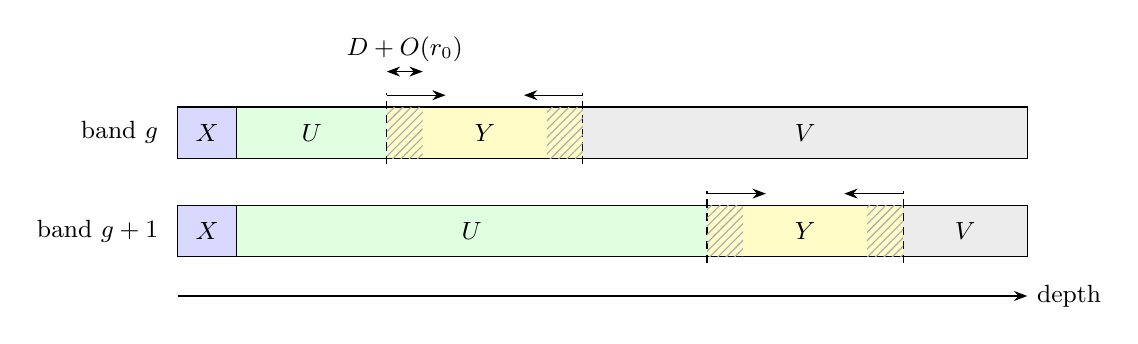
\begin{tikzpicture}[x=.83cm,y=1cm,font=\small,>=Stealth]
 \foreach \y/\leftfront/\rightfront/\band in
   {1.25/3.2/6.2/{g},0/8.1/11.1/{g+1}}{
  \fill[blue!15] (0,\y) rectangle (.9,{\y+.65});
  \fill[green!12] (.9,\y) rectangle (\leftfront,{\y+.65});
  \fill[yellow!22] (\leftfront,\y) rectangle (\rightfront,{\y+.65});
  \fill[gray!15] (\rightfront,\y) rectangle (13,{\y+.65});
  \draw (0,\y) rectangle (13,{\y+.65});
  \draw (.9,\y)--(.9,{\y+.65});
  \draw[densely dashed] (\leftfront,{\y-.08})--(\leftfront,{\y+.83});
  \draw[densely dashed] (\rightfront,{\y-.08})--(\rightfront,{\y+.83});
  \fill[pattern=north east lines,pattern color=gray!65]
       (\leftfront,\y) rectangle ({\leftfront+.55},{\y+.65});
  \fill[pattern=north east lines,pattern color=gray!65]
       ({\rightfront-.55},\y) rectangle (\rightfront,{\y+.65});
  \node at (.45,{\y+.325}) {$X$};
  \node at ({(.9+\leftfront)/2},{\y+.325}) {$U$};
  \node at ({(\leftfront+\rightfront)/2},{\y+.325}) {$Y$};
  \node at ({(\rightfront+13)/2},{\y+.325}) {$V$};
  \node[anchor=east] at (-.15,{\y+.325}) {band $\band$};
  \draw[->] (\leftfront,{\y+.8})--({\leftfront+.9},{\y+.8});
  \draw[->] (\rightfront,{\y+.8})--({\rightfront-.9},{\y+.8});
 }
 \draw[<->] (3.2,2.35)--node[above] {$D+O(r_0)$}(3.75,2.35);
 \draw[->] (0,-.5)--(13,-.5) node[right] {depth};
\end{tikzpicture}
\caption{Schematic nominal depth partitions in two bands, not to scale.
The horizontal coordinate records distance from the target, not a physical
lattice direction.  Dashed lines are the nominal fronts, and arrows show
the fill directions.  Charges may have assigned individual sites in the
hatched intervals, so the actual sets \(U,Y,V\) need not be depth
intervals.  The separated windows ensure that one support cannot split
two bands.  Every site of \(\Lambda\setminus A\) also belongs to \(V\)
in each band.  Auxiliary systems are not shown.}
\label{scanner:figure}
\end{figure}

\begin{lemma}[Geometry and probabilities of the scan]
\label{scanner:histories}
Under \eqref{scanner:scales}--\eqref{scanner:test-geometry}, the preceding
construction has the following properties for all sufficiently large \(n\).
\begin{enumerate}
\item Every splitting designated support is a graph \(r_0\)-ball wholly
inside \(A\).  It splits at most one band, and there it meets \(Y\)
and exactly one of the two sides.  The metric algebras generated by all
statuses of distinct bands commute on the symmetric replica space.
\item Every assigned site of \(A\) has oriented depth at most \(j+D+r_0\) on
its side.  Each actual set \(U\) or \(UY\) is comparable by inclusion
with a deterministic positive-depth prefix, and differs from that prefix
by at most \(CnD\) sites.  The cuts of \(U,UY,Y,P_0,V\) have at most
\(CnD\) edges.  At most \(CKnD\) terms split in any joint status.
\item For every labelled term \(i\), every round, and every common
\(p\), the sum of the full terminal-leaf probabilities on which it
splits is at most \(CD/m\).
\item An old history is called good if no side has an assigned site of \(A\) of
oriented depth greater than \(j+D/2\).  For every fixed \(M>0\), the
probability of a history failing this condition at any time is at most
\(n^{-M}\), for sufficiently large \(n\).  At a charge round on a good
old history, each split term is sampled on its splitting side with
probability at least \(c/(nD)\).
\end{enumerate}
All probabilities here are the classical path probabilities of the
history tree, before the transport of replica states.
\end{lemma}

\begin{proof}
\textbf{Deterministic geometry and nesting.}
A truncated support meeting \(S_0\) has radius \(r_0\): when its
anchor is at distance \(d>2r_0\), the alternative radius
\(\lfloor d/2\rfloor\) cannot reach \(S_0\).  Every splitting
support meets a compact part contained in \(S_0\), so this observation
applies.  If an \(r_0\)-ball meeting \(S_0\) also contained a site of
\(\Lambda\setminus A\), a graph path inside the ball would contain
a cut edge with an endpoint at ambient distance at most \(L+2r_0\)
from \(T\).  This contradicts \eqref{scanner:test-geometry}.

At a charge the largest newly assigned oriented depth is at most
\(j+D+r_0\); subsequent movement of the nominal front only improves
this bound.  Each side receives at most \(\lceil nm/2\rceil\) fills,
so advances through at most \(m/2+O(1)\) deterministic rows.  Its
charged lead is \(D+O(r_0)=o(m)\).  The two fronts in a window remain
separated by order \(m\), as do the active regions of successive
windows.  This proves both that an opposite side cannot have consumed
a scheduled slot and that a support cannot split two fronts.  All nonblank slots
strictly behind a nominal front have been assigned to that side.

A near set contains its completed deterministic prefix and is contained
in the prefix ending at its maximal allowed lead.  The difference has
at most \(CnD\) sites.  For \(UY\), take the complement of the
assigned far suffix within the original shell prefix: it is contained
in the deterministic prefix ending at the nominal far front and differs
from it only in \(O(D)\) rows.  These deterministic comparison prefixes
are all prefixes of one fixed ordered list of positive-depth slots and
are consequently nested, even across histories and bands.

A full depth prefix has \(O(n)\) boundary edges.  For its outer
boundary at positive depth, use the last included row, since depth
changes by at most one along an edge.  For the boundary at depth zero,
use the first positive row.  Partial rows cost at most \(4n\) more
edges.  There are no compact-to-opposite-color edges, by the clearance.
Changing at most \(CnD\) sites then gives the claimed \(O(nD)\)
bound for all status cuts and their differences.  Split anchors themselves
lie in \(O(D)\) rows around the nominal fronts, containing \(O(nD)\)
anchors per band.  Summing gives \(CKnD\).

For two bands \(g'<g''\), the entire near side together with the middle
of the first band is contained in the near side of the second band,
for every pair of histories.  After adjoining \(C\), this says
\(P_{g'}Y_{g'}\subset P_{g''}\).  Mirror the central function on
\(F_{g'}\) to its complement \(P_{g'}Y_{g'}\), using
Lemma~\ref{lem:schur}.  The resulting functions from the first band
commute with those of the second: they are disjoint from its \(Y,F\)
parts and invariant under the joint permutations whose center acts on
its \(P\) part.  This proves the asserted cross-band commutation.

\smallskip
\noindent\textbf{Dilution by the initial offsets.}
For a fixed anchor to split, its oriented depth must lie between
\(j-O(r_0)\) and \(j+D+O(r_0)\).  Both formulas in
\eqref{scanner:fronts} are affine, with coefficient \(1\) or \(-1\),
in the initial uniform offset.  Thus only \(O(D)\) of the \(m\)
offsets can permit this event, and only \(O(1)\) bands can reach the
fixed anchor.  This proves \(CD/m\) separately for the old and new
leaf distributions, and hence also for their common-\(p\) mixture.
It does not require conditional independence of the split event and
the later charge choices.

\smallskip
\noindent\textbf{Charge ancestry and availability.}
We finally bound the probability that charged sites get too far ahead of
a nominal front.  This will ensure that every old split lies in the
charge list.  Suppose a side has an assigned site of \(A\) leading
its nominal front by more than
\(D/2\).  Trace the site's first assignment backwards through the
charge ball that assigned it, choosing a previously assigned same-side
site in that ball, until an initial or deterministic assignment is
reached.  An ancestry with \(j'\) charges changes oriented depth by
at most \(2r_0j'\).  If its first charge is at time \(t_1\) and the
history is tested at time \(t\), then
\[
 2r_0j'>D/2+j(t)-j(t_1)-O(1).
\]
The fixed fill schedule gives
\(j(t)-j(t_1)\ge (t-t_1)/(4n)-O(1)\).  Substitution in the
preceding inequality yields both
\[
 j'\ge cD/r_0,\qquad t-t_1\le Cnr_0j'.
\]
Thus all ancestry times lie in this last interval of rounds.
All sites in the ancestry are in \(A\), including for the far side,
because the charging balls are wholly in \(A\).

For a fixed endpoint, test time, and length \(j'\), the time choices
and spatial choices have at most
\[
 \binom{\lceil Cnr_0j'\rceil}{j'}(Cr_0^4)^{j'}
\]
possibilities.  The spatial bound permits both an anchor and a
predecessor within \(O(r_0)\) graph distance at each step, and includes
the bounded anchor multiplicity.  Conditional on earlier choices, a
prescribed hit has probability at most \((cnD)^{-1}\).  The bound
\(\binom{v}{j'}\le(ev/j')^{j'}\) therefore makes the total probability
at most
\[
 \poly(n)\sum_{j'\ge cD/r_0}(Cr_0^5/D)^{j'}.
\]
The endpoints being counted are charged sites in \(S_0\), of which
there are \(O(n^2)\); the numbers of test times and bands are also
polynomial in \(n\).  Thus no far-domain volume enters this factor.
Since \(r_0\) is polylogarithmic and \(D=n^{\kappa+o(1)}\), the bound
is smaller than
every fixed inverse power of \(n\).

On a good old history, a split anchor has oriented depth at least
\(j-r_0\), because its ball meets an unassigned site, and at most
\(j+D/2+r_0\), because it meets the side.  For large \(n\) this
interval lies in the sampling interval \([j-r_0,j+D]\).  Choosing
the relevant side and its labelled slot has probability
\(1/(2M_n)\ge c/(nD)\), and the resulting move is exactly the
\(Y\)-part of that designated support.
\end{proof}

\subsection{Selecting a low-energy interpolation}

The scan provides the nested prefixes required by the norm comparisons
and the two probability estimates required by entropy and energy transport.
We now combine them to select one low-energy interpolation.  The entropy
input below concerns the original ground state; the polynomially accurate
truncation transfers it to \(\widetilde\Omega\).  No gap for a Hamiltonian
restricted to the target or its collar is used.

\begin{proposition}[The scanner estimate]
\label{prop:scanner}
Assume \eqref{scanner:scales} and \eqref{scanner:test-geometry}, and let
\(0<e<1\) satisfy \(\kappa\le e\).  Suppose
\begin{equation}
 S_\Omega(X)\le C_e n^{1+e},\qquad
 S_\Omega(Q_j)\le C_e(nL^e+n)\quad(0\le j\le L).
 \label{scanner:entropy-input}
\end{equation}
Let \(\epsilon=n^{-\nu}\), where \(\nu>0\) is fixed, and suppose
\(a r_0^2\) is sufficiently small.  Construct the auxiliary systems,
the fixed label sector, and the unnormalized vector \(\mathrm{pre}\)
as in Proposition~\ref{prop:comparators}, using typical width
\(w=n^{3/5}\).  For each sufficiently large replica count \(k\),
there are a charge round and a common parameter
\(p_k\in[\epsilon/2,\epsilon]\) at which the normalized vector
\(v_k=\mathcal M^{-s}\mathrm{pre}/N\), \(s=1/4\), has defect energy
\[
 E_{{\rm def},k}
 =\frac{\langle v_k,\overline{\widetilde H}v_k\rangle
                         -\widetilde E_0}{\widetilde g}
\]
bounded by
\begin{equation}
 E_{{\rm def},k}
 \le Cn^\ell D^2W^2(\log n)^C
        \bigl(\delta_n^{1/8}+\epsilon+n^{-100}\bigr)
        +Cn^{-1000}+o_k(1),
 \label{scanner:energy-output}
\end{equation}
where
\begin{equation}
 \delta_n=C_e\epsilon^{-1}
        \bigl(n^{e-\mu}+a^{1/4}(\log n)^C\bigr).
 \label{scanner:density-output}
\end{equation}
Here \(\overline{\widetilde H}\) is the mean of the physical
Hamiltonian over the copies.  All norm comparisons of
Proposition~\ref{prop:comparators} apply at the selected points, with
shell entropy bound \(B_{\rm sh}\le C_e(nL^e+n)\), mismatch
\(B_{\rm exc}\le CnD\), and marginal parameter
\(\mathcal B\le CnD(\log n)^C\).  The sharp comparisons additionally
require their stated condition on \(a\sqrt{\mathcal B}\).

The entire finite physical system, \(n\), the scan, and all auxiliary
dimensions are fixed before \(k\to\infty\).  The remainder is uniform
over the selected round and parameter, although these may depend on \(k\).
Constants may depend on the fixed exponents and the input constant \(C_e\).
\end{proposition}

\begin{proof}
The transfer from \(\Omega\) to \(\widetilde\Omega\) costs
\(O(n^{-248})\) in any entropy in \eqref{scanner:entropy-input}:
the trace distance is \(O(n^{-500})\), and the compact systems have
\(O(n^2)\) sites, so Lemma~\ref{lem:continuity} applies.  A partial
last depth row adds at most \(n\log q\).  Lemma~\ref{scanner:histories}
then gives the matched-prefix and mismatch bounds required by the
comparators.  It also gives the \(O(nD)\) status boundaries.  A
crossing support has Hilbert dimension at most \(q^{C(1+r_0)^2}\),
and its anchor lies within distance \(r_0\) of a cut edge.
Consequently the marginal-tail parameter of Lemma~\ref{lem:tail} is
at most \(CnD(\log n)^C\).  At the target itself it is at most
\(Cn(\log n)^C\).  The latter bound shows that the width \(w=n^{3/5}\)
has failure mass at most \(n^{-100}\) for all sufficiently large
\(n\).  In fact its tail is bounded by
\(C\exp[-c n^{1/10}/(\log n)^C]\).

At a charge round write \(h\) for an old joint history, of probability
\(w_h\), and \(\sigma_{h,u}\) for its transported state in
Proposition~\ref{prop:transport}.  Let \(\mu_\sigma\) denote the
coherent probability measure of Lemma~\ref{lem:symbol}.  The entropy
derivative uses the old-history weights \(w_h\); the same transported
states occur in the energy estimate with terminal weights \((1-p)w_h\).
We therefore measure the entropy cost of the old splits by
\(\mathcal Q(p)\), defined as
\begin{equation}
 \sum_{h\ {\mathrm{good}}}w_h
  \int_{\R}m_s(u)
   \int\sum_{i\ {\mathrm{split\ in}}\ h}
       \eta_{i,h}(\theta)\,d\mu_{\sigma_{h,u}}(\theta)\,du.
 \label{scanner:Q-definition}
\end{equation}
Each split term in this sum has a unique splitting band, and its
partition \(P,Y,F\) is understood to be that band's partition.
If term \(i\) splits on the near side, its moved set is
\(x=Y\cap\widetilde X_i\), the unassigned part of its designated
\(r_0\)-ball, and
\(\eta_{i,h}=S_\theta(x\mid P)+S_\theta(x\mid Y\setminus x)\);
on the far side exchange \(P,F\).  These quantities are nonnegative.
They are also bounded by \(C(\log n)^C\), because the moved sites lie
in an \(r_0\)-ball.  The measure \(m_s(u)\,du\) has fixed finite
mass \(2s\).

On every good old history each split term is sampled with probability
at least \(c/(nD)\), and its sampled move has exactly the corresponding
\(\eta_{i,h}\).  Equation~\eqref{transport:entropy-gain} therefore
gives, at a charge round,
\begin{equation}
 -\partial_p\log N^2
 \ge \frac{cka}{nD}\mathcal Q(p)
       -CkaK a^{1/4}(\log n)^C-O_{\rm fixed}(\log(k+2)).
 \label{scanner:charge-gain}
\end{equation}
At fill rounds retain just the same negative error; the entropy gains
are nonnegative.  Here and below ``fixed'' means that the complete
single-copy instance and the scanner have been fixed.  No such
constant survives the replica limit.

Integrate over every full round, including fills.  Adjacent endpoint
metrics agree by construction, so the left sides telescope.  Initially
\(-\log N^2\ge-O_{\rm fixed}(\log(k+2))\): the floor
\eqref{replicas:leaf-floor} passes to the initial mean tree by
Lemma~\ref{transport:means}, and \(\|\mathrm{pre}\|\le1\).
At the last endpoint the rough
upper comparison \eqref{comparator:rough-upper} gives
\[
 -k^{-1}\log N^2
 \le 2\log d_*-\log z+C_eW(nL^e+nD+n)+o_k(1)
 \le C_eW n^{1+e}+o_k(1).
\]
For the last inequality use \(\kappa\le e\), \(L\le n\), and
\(\log d_*=S_{\widetilde\Omega}(X)+O(w+|\log z|)\).
Restrict the positive charge integrals in
\eqref{scanner:charge-gain} to \([\epsilon/2,\epsilon]\), but pay
the negative errors on all \(2nm\) full rounds.  Since \(aK=W\),
the integrated inequality, normalized by the number of charge rounds, is
\[
 \frac1{nm}\sum_{\text{charge rounds}}
  \int_{\epsilon/2}^{\epsilon}\frac{\mathcal Q(p)}{KnD}\,dp
 \le C_e\left(\frac{n^e}{m}+a^{1/4}(\log n)^C\right)+o_k(1).
\]
The interval has length \(\epsilon/2\), and \(m\asymp n^\mu\).
Averaging therefore gives a charge round and a \(p_k\) in this interval
such that
\begin{equation}
 \frac{\mathcal Q(p_k)}{KnD}\le\delta_n+o_k(1).
 \label{scanner:selected-density}
\end{equation}
The fixed factor two in the interval length is absorbed into constants.
All integrands are bounded at fixed \(k\), and continuous in the
interior interpolation parameter, so ordinary averaging suffices for
this selection.

Apply the energy estimate \eqref{transport:energy} at this same point.
For each term its split weight is at most \(CD/m\).  There are at
most \(CKnD\) split term occurrences in each joint leaf.  On old
good leaves the transported states are exactly those in
\eqref{scanner:Q-definition}; their full terminal weight differs only
by the factor \(1-p_k\le1\).  H\"older's inequality, applied to the
positive measure over histories, terms, \(u\), and \(\theta\), bounds
their sum of \(\eta^{1/8}\) by
\[
 CKnD\bigl(\delta_n+o_k(1)\bigr)^{1/8}.
\]
On bad old histories use the uniform local dimension bound and
Lemma~\ref{scanner:histories} with an arbitrarily large fixed tail
power.  On all new leaves use the same dimension bound and their
total terminal weight \(p_k\le\epsilon\).  After increasing the fixed
logarithmic power, the energy estimate is therefore
\[
 \langle v_k,\overline{\widetilde H}v_k\rangle
 \le 2\widetilde E_0+
 C a^2\frac Dm KnD(\log n)^C
       \bigl(\delta_n^{1/8}+\epsilon+n^{-100}\bigr)+o_k(1).
\]
The factors in this expression have distinct origins: \(D/m\) is the
split probability of one fixed term, \(KnD\) counts split occurrences,
and \(a^2\) is the local skew cost.  Their product simplifies to
\[
 a^2\frac Dm KnD
   =\frac{W^2nD^2}{mK}
   \le CW^2n^\ell D^2.
\]
Subtracting \(\widetilde E_0\) and dividing by
\(\widetilde g\ge g/2\) proves
\eqref{scanner:energy-output}.

Only splitting terms contribute to this energy error; all others have
zero skew exactly.  Thus its coefficient contains no total-volume
factor.  The symbol remainders can be summed over all terms before
taking \(k\to\infty\), because that complete term set is finite and
fixed.  Their uniformity in replica states and in the interpolation
parameter also justifies the possibly \(k\)-dependent selection in
\eqref{scanner:selected-density}.
\end{proof}

\subsection{Geometric targets and entropy inputs}

We now supply the scanner's geometric and entropy inputs for unions of
rectangles and triangles.  These include the geometric targets of the final
tiling, whose number of pieces may grow with the scale.  The constant
\(D_0\) and the function \(F_{\rm box}\) are those of
Proposition~\ref{prop:initial-box}.  Fix the numerical constant
\(C_{\rm tpl}\) large enough to absorb the layer-count constant in the
proof below.  The entropy bounds will be reused each time the safe-box
exponent improves.

\begin{definition}[A template]
\label{scanner:template}
Let \(s_0\ge1\) and \(n\) be positive integers.  A template with parameters
\((n,s_0)\) is a nonempty finite set \(T\subset\Z^2\) of the form
\[
 T=\bigcup_{a=1}^{N_0}(P_a\cap\Z^2),
 \qquad n\ge C_{\rm tpl}N_0(s_0+1),
 \qquad \diam_\infty T\le n,
\]
where \(N_0\ge1\) is an integer and each \(P_a\) is a closed convex rectangle or triangle of sup-norm
diameter at most \(s_0\), all of whose sides have slope
\(0,\infty,1\), or \(-1\).  Empty sampled pieces can be omitted.
For the fixed cut \(A\), the template is separated from the cut if
\[
 \dist_\infty(T,Z)>4D_0s_0.
\]
As above, \(T_j\) is the ambient integer dilation,
\(X=A\cap T\), and \(Q_j=A\cap(T_j\setminus T)\), for \(j\ge0\).
\end{definition}

The diameter condition merely fixes a convenient common size parameter.
The estimates below use the number and sizes of the pieces, rather than
convexity of their union.  They therefore allow the disconnected fragments
which occur in the later tiling.

\begin{lemma}[Rows, coverings, and shell entropy]
\label{scanner:templates}
For \(C_{\rm tpl}\) sufficiently large, a template satisfies
\begin{equation}
 |T|\le Cns_0,\qquad
 |T_j\setminus T_{j-1}|\le n\quad(1\le j\le s_0),
 \qquad |\partial_{\Z^2}T_j|\le Cn\quad(0\le j\le s_0).
 \label{scanner:template-geometry}
\end{equation}
Suppose it is separated from the cut and, for some \(0<e<1\),
\(F_{\rm box}(r)\le C_e r^{1+e}\) for every integer \(r\ge1\).
Then, for every integer \(1\le L\le s_0\),
\begin{equation}
 S_\Omega(X)\le C'_e ns_0^e,\qquad
 S_\Omega(Q_j)\le C'_e nL^e\quad(0\le j\le L).
 \label{scanner:template-entropy}
\end{equation}
The same shell bound, with an additional \(Cn\), holds for any prefix
obtained by including all depth rows before one row and an arbitrary
subset of that last row.  All physical cuts of \(X,Q_j\), and
\(A\cap T_j\) have \(O(n)\) edges.
\end{lemma}

\begin{proof}
Consider first one sampled piece.  On an integer horizontal row its sites
form an integer interval.  Its left endpoint is a maximum of affine
integer-valued functions with slopes in \(\{-1,0,1\}\), and its right
endpoint is a minimum of such functions; horizontal sides impose an
interval constraint on the row index.  To obtain these formulas, round
the intercepts of the defining line inequalities.  Because the slopes
are integers, this rounding is independent of the integer row index.
The difference of the lower and upper bounds is convex, so the nonempty
rows are consecutive.  On consecutive nonempty rows each endpoint moves
by at most one.  Consecutive row intervals overlap or are adjacent as
integer intervals.

After integer sup-norm dilation by \(j\), the interval on a row is the
union of the original intervals in the window of rows at distance at
most \(j\), each extended by \(j\) on both ends.  This union is still
an integer interval.  Its endpoints are the sliding minimum and maximum
of the old endpoints, minus or plus \(j\).  They again move by at most
one between consecutive nonempty rows: the nonempty index windows at
two consecutive rows have Hausdorff distance at most one, and the old
endpoint functions are 1-Lipschitz.  One more dilation changes each
endpoint on an old row by at most two and adds at most two rows, each
of length \(O(s_0+j+1)\).  This proves a bound
\(C(s_0+j+1)\) for both the new layer and the edge boundary of one
piece.  Summing over the pieces proves
\eqref{scanner:template-geometry}, with the layer constant absorbed in
\(C_{\rm tpl}\).  The area bound follows from
\(|P_a\cap\Z^2|\le C(s_0+1)^2\).

We also need a count at intermediate dyadic scales.  In the usual dyadic
partition of the lattice into integer squares, the number of side-\(u\)
squares containing both a site of a dilated piece and a site outside it
is
\begin{equation}
 O\bigl((s_0+j+1)/u+1\bigr),\qquad u\ge1.
 \label{scanner:mixed-piece}
\end{equation}
Indeed, in a block of \(u\) consecutive nonempty rows the two endpoints
vary by at most \(u\).  Only constantly many square columns near each
endpoint can be mixed.  At the first and last blocks count instead the
whole width, which costs \(O((s_0+j+1)/u+1)\) in total.
A square mixed for a union, or for a difference of two unions, must be
mixed for at least one of the constituent sets.  Thus the corresponding
count for \(T\), \(T_j\), or \(T_j\setminus T\), with \(j\le s_0\),
is at most
\(C(N_0+n/u)\).

Cover \(T_j\setminus T\) by maximal contained dyadic squares, with side
capped at the largest power of two not exceeding \(L\).  These squares
partition the set: a single site is an admissible square, and the dyadic
nesting makes distinct maximal squares disjoint.  At the cap there are
at most \(Cn/L\) squares because
\(|T_j\setminus T|\le nj\le nL\).  Below the cap, the parent of each
maximal square is mixed.  Equation~\eqref{scanner:mixed-piece} therefore
bounds the number of squares of side \(u\) by
\(C(N_0+n/u)\le Cn/u\), since \(u\le L\le s_0\) and
\(N_0s_0\le n\).  All these squares are safe: their sites lie in
\(T_j\), their sides are at most \(s_0\), and
\[
 \dist_\infty(T_j,Z)\ge\dist_\infty(T,Z)-j
   >4D_0s_0-s_0>D_0s_0.
\]
Subadditivity and the assumed box bound now give
\[
 S_\Omega(Q_j)
 \le C_e n\sum_{\substack{u\le L\\u\ \mathrm{dyadic}}}u^e
 \le C'_e nL^e.
\]
Covering \(T\) in the same way, with cap comparable to \(s_0\),
uses \(O(n/s_0)\) squares at the cap and \(O(n/u)\) below it, and
gives the first bound in \eqref{scanner:template-entropy}.

Adding an arbitrary part of one depth row changes entropy by at most
\(n\log q\).  Finally, near these sets there is no edge joining \(A\)
to its complement: such an edge would have an endpoint in \(Z\) within
distance \(s_0+1\) of \(T\).  Thus their physical boundaries are bounded
by the ambient template and shell boundaries just counted.  This argument
does not count missing lattice edges as physical boundary edges.
\end{proof}

\subsection{A small safe-box exponent}

We use the scanner first with a bounded total metric weight.  The rough
comparison is sufficient here, even when \(a\sqrt{\mathcal B}\) is
large.  This separates the bootstrap from the sharper concentration
condition needed only in the final application.

\begin{proposition}[Improved safe-box estimate]
\label{prop:small-box}
There is a constant \(C\), depending only on the Hamiltonian parameters,
such that
\[
 F_{\rm box}(r)\le Cr^{1+e_*}\quad(r\ge1),
 \qquad e_*=2\cdot10^{-6}.
\]
\end{proposition}

\begin{proof}
Let \(e_0\in(0,1)\) be supplied by
Proposition~\ref{prop:initial-box}.  If \(e_0\le e_*\), the assertion
already follows.  Otherwise fix, once for the entire bootstrap,
\begin{equation}
 g_0=(1-e_0)/2,
 \quad \mu=1-g_0,
 \quad \nu=g_0/1000,
 \quad \ell=\nu/100,
 \quad \kappa=\min(\nu/100,e_*/4),
 \quad W=4.
 \label{scanner:bootstrap-parameters}
\end{equation}
These parameters will not change when the current entropy exponent
improves.

Suppose \(F_{\rm box}(r)\le C_e r^{1+e}\), where
\(e_*<e\le e_0\).  Take any safe integer rectangle \(T\) of actual
maximal side length \(s_0\), and set \(n=\lceil C_2s_0\rceil\)
for a sufficiently large fixed \(C_2\).  If \(A\cap T\) is empty,
its entropy is zero, so assume otherwise.  For large \(s_0\),
\(L=o(s_0)\), so \eqref{scanner:test-geometry} holds.  In particular
the weaker safe-box clearance \(D_0s_0\), rather than the stronger
template clearance of Definition~\ref{scanner:template}, is enough
for this application.

Here is the shell entropy input explicitly.  The shell
\(T_j\setminus T\), \(j\le L\), has area \(O(nL)\) and consists
of a bounded number of rectangular strips.  Its mixed dyadic squares
of side \(u\) number \(O(n/u+1)\), by the boundary-line count.
The maximal-contained-square argument of
Lemma~\ref{scanner:templates}, capped at side comparable to \(L\),
therefore gives \(S_\Omega(Q_j)\le C_e nL^e\).  These covering
squares are safe: their sides are at most \(L\), and their distance
from \(Z\) is at least \(D_0s_0-L>D_0L\) once \(s_0\) is large.
This also covers thin rectangles.  The target entropy is at most
\(C_e s_0^{1+e}\).  Adding a partial row costs \(O(n)\), so all
the hypotheses of Proposition~\ref{prop:scanner} hold.

We check its quantitative output.  Since
\(K\asymp n^{g_0-\ell}\),
\(a\asymp n^{-g_0+\ell}\).  In
\eqref{scanner:density-output} the two powers before logarithms are
at most
\[
 e_0-\mu+\nu=-0.999g_0,
 \qquad -(g_0-\ell)/4+\nu=-0.2489975g_0.
\]
Thus \(\delta_n\le n^{-0.24g_0}\) for sufficiently large \(n\),
after constants and fixed logarithmic powers have been absorbed.
The energy prefactor has power
\(\ell+2\kappa\le0.00003g_0\).  Its slower decaying input is
\(\epsilon=n^{-0.001g_0}\), rather than
\(\delta_n^{1/8}\le n^{-0.03g_0}\).  Hence
\begin{equation}
 E_{{\rm def},k}\le Cn^{-\nu/2}+o_k(1).
 \label{scanner:bootstrap-energy}
\end{equation}
All scale conditions and the smallness of \(ar_0^2\) hold at large
\(n\).  No sharp marginal-moment condition has been used.

Put \(\tau=n^{-\nu/4}\).  Apply the rough upper and lower
comparisons \eqref{comparator:rough-upper} and
\eqref{comparator:rough-lower} at the selected interpolation.  Write
\(S_X=S_{\widetilde\Omega}(X)\).  The upper pin cost has leading
coefficient \(2S_X\); the lower coefficient is
\(4sWS_X=4S_X\).  Replacing \(\log d_*\) and \(S'\) by \(S_X\)
costs \(O(w+|\log z|)\).  The remaining relative loss in this
coefficient is at most
\(C(\tau+E_{{\rm def},k}/\tau)\), which is small after taking
\(k\to\infty\) and then \(n\) sufficiently large.  The two
comparisons consequently imply
\begin{equation}
 S_X\le C_e\bigl(nL^e+nD+w+h(\tau)/a+1\bigr).
 \label{scanner:bootstrap-comparison}
\end{equation}
To justify the order of limits in this absorption, keep \(n\) fixed
in both norm comparisons and use
\eqref{scanner:bootstrap-energy}.  The resulting scalar inequality
has the same \(S_X\) for every \(k\); all other remainders are
uniform at the selected points and vanish.  Only then choose the
large-scale threshold making the coefficient loss smaller than the
fixed margin between four and two.

For \(0<\tau<1/2\), \(h(\tau)\le C\tau\log(e/\tau)\).  Therefore
\[
 h(\tau)/a
 \le C n^{g_0-\ell-\nu/4}\log n=O(n),
\]
because \(g_0<1/2\).  Also \(w=n^{3/5}\le n\), and
\(\kappa\le e_*/4<(1-\ell)e\) while \(e>e_*\).
Equation~\eqref{scanner:bootstrap-comparison}, followed by the
negligible transfer back to \(\Omega\), gives
\[
 S_\Omega(A\cap T)\le C'_e n^{1+(1-\ell)e}
                       \le C''_e s_0^{1+(1-\ell)e}.
\]
Bounded \(s_0\) are included by increasing the constant, using the
volume bound.  Taking the supremum over safe boxes thus replaces
the current exponent \(e\) by \((1-\ell)e\).

Starting from \(e_0\), finitely many repetitions reach an exponent
at most \(e_*\), which can be loosened to \(e_*\).  Every iteration
uses only the current safe-box estimate on the shell covering squares.
The parameters in \eqref{scanner:bootstrap-parameters}, and the finite
number of iterations, depend only on the fixed Hamiltonian parameters.
Thus the final constant is uniform over the domain and cut.
\end{proof}

\subsection{The collar mutual information}

After the bootstrap we allow the total metric weight to grow slowly.
The exact norm comparison then charges the remaining target pin cost by
the reciprocal of that weight.  This is the point at which the entropy
identity in Proposition~\ref{prop:comparators} gives a bound independent
of the selected history.

\begin{proposition}[A sublinear collar bound]
\label{prop:collar}
Let \(T\) be a template separated from the cut, with parameters
\((n,s_0)\) as in Definition~\ref{scanner:template}.  Set
\[
 L=\lfloor n^{1-10^{-5}}\rfloor,
 \qquad X=A\cap T,
 \qquad S_0=A\cap T_L,
\]
and suppose \(L\le s_0\).  For all sufficiently large \(n\),
\begin{equation}
 I_\Omega(X:\Lambda\setminus S_0)
       \le C n^{1-\varepsilon},\qquad \varepsilon=10^{-5}.
 \label{scanner:collar-output}
\end{equation}
The constant and threshold are independent of \(T,s_0,n,\Lambda\),
and \(A\).  The cuts of \(X,S_0\), and \(S_0\setminus X\) have
\(O(n)\) edges, and \(|S_0|=O(n^2)\).
\end{proposition}

\begin{proof}
If \(X\) is empty there is nothing to prove.  Otherwise
Proposition~\ref{prop:small-box} and
Lemma~\ref{scanner:templates} supply
\eqref{scanner:entropy-input} with \(e=e_*=2\cdot10^{-6}\).
Since \(s_0\le n\), the core entropy is at most \(Cn^{1+e}\).
The template clearance and \(L\le s_0\) imply
\eqref{scanner:test-geometry} at large \(n\); the logarithmic
truncation radius is negligible compared with \(L\).

Use the following fixed parameter choices:
\begin{equation}
 \mu=\frac14,\quad \nu=\frac1{1000},\quad
 \ell=\frac1{100000},\quad
 \omega=\frac1{20000},\quad
 \kappa=\frac1{1000000},\quad W=n^\omega.
 \label{scanner:final-parameters}
\end{equation}
Then \(a\asymp n^{-0.74994}\).  The two terms in
\eqref{scanner:density-output} have powers
\(-0.248998\) and \(-0.186485\), before the fixed logarithmic
factors.  Hence \(\delta_n\le n^{-0.18}\) at sufficiently large
scales.  The power of the energy prefactor is
\[
 \ell+2\kappa+2\omega=0.000112.
\]
The \(\epsilon=n^{-0.001}\) term is again the limiting one, and
Proposition~\ref{prop:scanner} gives
\begin{equation}
 E_{{\rm def},k}\le Cn^{-0.0005}+o_k(1).
 \label{scanner:final-energy}
\end{equation}
Set \(\tau=n^{-0.00025}\).  All fixed multiples of \(a\) lie in
the marginal-moment interval required for the sharp comparisons,
since
\[
 a\sqrt{\mathcal B}
 \le C n^{-0.2499395}(\log n)^C\longrightarrow0.
\]

At each leaf write, as before, the physical partition as \(X,U,Y,V\).
All entropies in the next calculation refer to \(\widetilde\Omega\).
Let
\[
 g_{\rm pre}=S(XU)+S(V)-S(Y),\qquad
 g_{\rm post}=S(U)+S(UY)-S(Y).
\]
These are the quantities in the sharp norm comparisons.  Their upper
bounds are uniform in the status.  In particular
\(S(XU)\le S(X)+S(U)\le Cn^{1+e}\), and by purity
\(S(V)=S(XUY)\le S(X)+S(UY)\le Cn^{1+e}\).
Here the matched-prefix error \(CnD\) is absorbed because
\(\kappa<e\).  Thus \(0\le g_{\rm pre}\le Cn^{1+e}\).

Denote the full terminal path and uniform band average by
\(\langle\cdot\rangle_{\rm leaf}\).  Subtracting
\eqref{comparator:sharp-upper} from
\eqref{comparator:sharp-lower}, and then dividing by \(2sW\), bounds
\(2S(X)+\langle g_{\rm pre}-g_{\rm post}\rangle_{\rm leaf}\)
by a constant times
\begin{equation}
 \frac{S(X)+1}{W}+w
 +(\tau+E_{{\rm def},k}/\tau)n^{1+e}
 +\frac{h(\tau)}a+a\mathcal B
 +\frac{|\log z|}a+o_k(1).
 \label{scanner:final-errors}
\end{equation}
This calculation uses \(S'=S(X)+O(w+|\log z|)\) and the analogous
estimate for \(\log d_*\).  It also restores the lost
\(\tau\langle g_{\rm pre}\rangle_{\rm leaf}\) from the lower
comparison using the preceding uniform bound.

For each leaf separately, purity gives the exact identity
\begin{equation}
 2S(X)+g_{\rm pre}-g_{\rm post}
       =I(X:V)+I(X:YV).
 \label{scanner:entropy-identity}
\end{equation}
Both \(V\) and \(YV\) contain the fixed subsystem
\(\Lambda\setminus S_0\).  Monotonicity of mutual information
therefore makes the left side of \eqref{scanner:entropy-identity}
at least \(I_{\widetilde\Omega}(X:\Lambda\setminus S_0)\),
independently of the history.  This remains true after the leaf average,
even though the selected round and its weights can vary with \(k\).

For completeness, after \(k\to\infty\) the terms in
\eqref{scanner:final-errors} have the following upper bounds on their
powers of \(n\), apart from fixed logarithms.
\begin{center}
\begin{tabular}{@{}lc@{}}
\toprule
Error term & Power of $n$\\
\midrule
$(S(X)+1)/W$ & $0.999952$\\
$w$ & $0.6$\\
$(\tau+E_{{\rm def},k}/\tau)n^{1+e}$, after $k\to\infty$ & $0.999752$\\
$h(\tau)/a$ & $0.74969$\\
$a\mathcal B$ & $0.250061$\\
$|\log z|/a$ & $-99.25006$\\
\bottomrule
\end{tabular}
\end{center}
All are strictly below \(1-\varepsilon=0.99999\).
Equation~\eqref{scanner:final-energy} controls the mass-loss term
uniformly before the limit.  This proves
\(I_{\widetilde\Omega}(X:\Lambda\setminus S_0)
\le Cn^{1-\varepsilon}\).

Finally write mutual information as
\(S(X)-S(X\mid\Lambda\setminus S_0)\) and use
Lemma~\ref{lem:continuity}.  Only \(\log\dim\mathcal H_X=O(n^2)\)
enters, even if the far subsystem is very large.  The trace distance
\(O(n^{-500})\) between the original and truncated ground states
therefore changes this mutual information by \(O(n^{-248})\).
This proves \eqref{scanner:collar-output}.  The final size and boundary
assertions were established in Lemma~\ref{scanner:templates}.
\end{proof}

The replica construction has now been eliminated: the conclusion of
Proposition~\ref{prop:collar} is an inequality for the original finite
ground state.  The next section applies the exact positive quasi-local
system to that state.  In particular, the exponentially large auxiliary
operator used there never multiplies a truncation or a replica error
from the present argument.

\section{Amplifying the collar estimate}\label{sec:amplification}

Proposition~\ref{prop:collar} gives a sublinear bound on the mutual
information between a target and the region beyond its collar.  We now
make this mutual information smaller than any fixed inverse power of
the scale, at the cost of a slightly wider collar.  Typical spectral
subspaces first give a candidate restoring operator whose norm is
controlled by the collar mutual information.  Positive constraints
suppress its excited component, yielding accurate restoration after
localization.  A polar decomposition then replaces this operator by a
local unitary.  An untouched reference copy records the target's
correlations with the remote system and witnesses their decoupling.

Throughout this section fix
\begin{equation}\label{eq:amplification-exponents}
 \varepsilon=10^{-5},\qquad \beta=1-2\cdot10^{-6},\qquad
 \alpha=\frac{p}{p+1}>1-10^{-6},
\end{equation}
where the integer $p$ is fixed.  Apply Proposition~\ref{prop:positive}
with this value of $p$.  Thus, in this section, $H_F=\sum_i k_i$ is a
fresh exact positive system with
\begin{equation}\label{eq:amplification-positive-system}
 0\le k_i\le I,\quad k_i\Omega=0,\quad
 H_F\ge g(I-P_\Omega),\qquad
 P_\Omega=|\Omega\rangle\langle\Omega|,
\end{equation}
and $g>0$ is independent of the finite domain.  The scanner's
truncated Hamiltonian is no longer used.  All neighborhoods below are
neighborhoods in the induced graph: for $S\subseteq\Lambda$ we write
$N_r(S)=\{y\in\Lambda:d_\Lambda(y,S)\le r\}=N_r^\Lambda(S)$.

\subsection{Localizing products of positive constraints}

The following estimate supplies the localization needed later.  It is
stated for a general operator, which may act on additional finite
systems.  These additional systems are spectators in the dynamics.
The spatial truncation argument has the propagation structure of
dissipative Lieb--Robinson estimates~\cite[Theorems~1 and~2]{BarthelKliesch2012}.
We prove it here on coupled clock realizations, since the needed bound
is an expectation of a norm.

\begin{lemma}[Local constraint products]\label{lem:amplification-local-products}
Let positive contractions $k_i$, anchored at $a_i\in\Lambda$ with
bounded multiplicity, satisfy
\[
 \|k_i-E_{i,l}k_i\|\le C e^{-c l^\alpha}\qquad(l\ge0),
\]
where $E_{i,l}$ is conditional expectation onto $N_l(a_i)$.
Set $G_i=(I-k_i)^{1/2}$ and $K_i=k_i^{1/2}$.
Fix $t\ge0$ and an integer $r\ge1$.
At each anchor label run an independent rate-one Poisson clock on
$[0,t]$.  In occurrence order, with later factors on the left, let
$D$ be the product of all $G_i$, and let $D_{\rm ret}$ retain only
events with $d_\Lambda(a_i,S)\le r$, for a nonempty set $S\subseteq\Lambda$.
Let $L$ be the same retained product with each $G_i$ replaced by
$G_{i,r}=(I-E_{i,r}k_i)^{1/2}$.

There are uniform constants $C,c,v>0$ such that
\begin{equation}\label{eq:amplification-product-truncation}
 \mathbb E\|D_{\rm ret}-L\|
 \le Ct|S|(1+r)^2e^{-c r^\alpha}.
\end{equation}
In particular $L$ is a contraction supported on $N_{2r}(S)$.
If $k_i\Omega=0$ and an operator $B$ is supported on $S$ and
spectator systems, then, for every unit spectator vector $\xi$,
\begin{equation}\label{eq:amplification-product-omission}
 \mathbb E\|(D-D_{\rm ret})B(\Omega\otimes\xi)\|
 \le Ct|S|\|B\|e^{vt-c r^\alpha}.
\end{equation}
Both bounds concern the same coupled clock realization.  Their constants
are independent of $|\Lambda|$ and of spectator dimensions.
\end{lemma}

\begin{proof}
We first prove an operator estimate for unital channels.  Define
\[
 \mathcal E_i(B)=G_iBG_i+K_iBK_i,
 \qquad
 \mathcal E_{i,l}(B)=G_{i,l}BG_{i,l}+K_{i,l}BK_{i,l},
\]
where $K_{i,l}=(E_{i,l}k_i)^{1/2}$.  When $k_i\Omega=0$, functional
calculus gives $G_i\Omega=\Omega$ and $K_i\Omega=0$, so
\begin{equation}\label{eq:amplification-channel-vector}
 \mathcal E_i(C)(\Omega\otimes\xi)=G_iC(\Omega\otimes\xi)
\end{equation}
for every operator $C$ and spectator vector $\xi$.  Products of these
channels therefore recover the contraction products when evaluated on
the ground vector.  We localize the channels first: their unitality
makes each local channel fix the algebra outside its supporting ball.
They are also completely positive, hence contractions in operator norm,
including after adjoining spectators.  Lemma~\ref{lem:quasilocal-roots} gives
\begin{equation}\label{eq:amplification-channel-approximation}
 \|\mathcal E_i-\mathcal E_{i,l}\|_{\rm cb}
 \le C e^{-c l^\alpha}.
\end{equation}
The completely bounded norm here is the supremum of the operator norms
after adjoining identity maps on finite spectator systems.  In this
case the estimate follows directly from the norm bounds for the two
square roots, so it has no dimension factor.

Put $\mathcal E_{i,-1}=\id$ and
$\Delta_{i,l}=\mathcal E_{i,l}-\mathcal E_{i,l-1}$ for $l\ge0$.
By increasing $C$ to include $l=0$,
\begin{equation}\label{eq:amplification-channel-shells}
 \|\Delta_{i,l}\|_{\rm cb}\le C e^{-c l^\alpha}.
\end{equation}
Both channels in this difference fix operators commuting with the
algebra on $N_l(a_i)$.  Thus the difference vanishes on that
commutant.  For an operator $B$ define its oscillation at a physical
site $y$ by
\[
 d_y(B)=\sup_{U_y\ {\rm unitary}}\|[U_y,B]\|.
\]
Average over the on-site unitaries in a set $Q$, one site at a time.
The total norm change is at most $\sum_{z\in Q}d_z(B)$, and the result
commutes with the algebra on $Q$.  Consequently
\begin{equation}\label{eq:amplification-shell-oscillation}
 \|\Delta_{i,l}(B)\|
 \le C e^{-c l^\alpha}\sum_{z\in N_l(a_i)}d_z(B).
\end{equation}
This argument also applies to operators acting on spectators.

To bound the oscillation after one event, suppose first that
$m=d_\Lambda(a_i,y)<\infty$.  The channel $\mathcal E_{i,m-1}$
does not act at $y$ and commutes with conjugation by $U_y$; hence it
cannot increase $d_y$.  Telescope the shells from radius $m$ onward
and use $d_y(C)\le2\|C\|$ to obtain
\begin{equation}\label{eq:amplification-oscillation-increment}
 d_y(\mathcal E_i B)\le d_y(B)+
 C\sum_{l\ge d_\Lambda(a_i,y)}e^{-c l^\alpha}
       \sum_{z\in N_l(a_i)}d_z(B).
\end{equation}
For $m=0$ the initial channel is the identity.  If $m=\infty$,
$\mathcal E_i$ acts in a different component and cannot increase
$d_y$.  Exact component support follows either from the construction
or by letting $l$ exceed the component diameter in the approximation
assumption.

Sum the increment in
\eqref{eq:amplification-oscillation-increment} over the retained
anchor labels.  Define the nonnegative matrix
\[
 A_{yz}=C\sum_{i\ {\rm retained}}\sum_{l\ge0}
 e^{-cl^\alpha}\mathbf1_{\{y,z\in N_l(a_i)\}},
\]
with the constant from \eqref{eq:amplification-oscillation-increment}.
It has a uniformly bounded weighted row sum:
\begin{equation}\label{eq:amplification-weighted-kernel}
 \sup_y\sum_{z:\,d_\Lambda(y,z)<\infty}
 A_{yz}e^{a d_\Lambda(y,z)^\alpha}\le v
\end{equation}
for some $a>0$.  Indeed, at radius $l$ there are at most
$C(1+l)^2$ anchor labels whose balls contain $y$, and at most
$C(1+l)^2$ sites in each ball.  Their distances from $y$ are at most
$2l$.  The left side is therefore bounded by
\[
 C\sum_{l\ge0}(1+l)^4e^{-c l^\alpha+a(2l)^\alpha},
\]
which is finite for sufficiently small $a$.  There are no kernel
entries between different components.

Let $B_u$ be the result of the retained channel events up to time $u$,
starting from $B$.  The Poisson jump formula and
\eqref{eq:amplification-oscillation-increment} imply, in integral
form, the differential upper bound
\[
 \frac{d}{du}\mathbb E d_y(B_u)
 \le\sum_z A_{yz}\mathbb E d_z(B_u).
\]
The site and anchor sums are finite for a fixed domain, and the radius
sums converge absolutely with the uniform bounds in
\eqref{eq:amplification-weighted-kernel}.
Initially $d_y(B)\le2\|B\|1_S(y)$.  On components meeting $S$,
weight the last inequality by $e^{a d_\Lambda(y,S)^\alpha}$.
The triangle inequality and $0<\alpha<1$ give
\[
 d_\Lambda(y,S)^\alpha-d_\Lambda(z,S)^\alpha
 \le d_\Lambda(y,z)^\alpha.
\]
The weighted supremum thus grows at rate at most $v$.
Gronwall's inequality yields
\begin{equation}\label{eq:amplification-propagation}
 \mathbb E d_y(B_u)
 \le2\|B\|e^{vu-a d_\Lambda(y,S)^\alpha}.
\end{equation}
Oscillations on components disjoint from $S$ remain zero.

We can now remove the distant events.  For an omitted anchor at finite
distance $d=d_\Lambda(a_i,S)>r$, sum
\eqref{eq:amplification-shell-oscillation} over all $l\ge0$ and
apply \eqref{eq:amplification-propagation}.  When $l\le d/2$,
every $z\in N_l(a_i)$ has $d_\Lambda(z,S)\ge d/2$.
The sum over these radii is bounded by
$C\|B\|e^{vu-a(d/2)^\alpha}$.  For $l>d/2$ use the shell
decay and the ball cardinality instead.  Absorbing its polynomial
factor gives, in both cases,
\begin{equation}\label{eq:amplification-omitted-event}
 \mathbb E\|(\mathcal E_i-\id)(B_u)\|
 \le C\|B\|e^{vu-c'd^\alpha}.
\end{equation}
At infinite distance the left side is zero.

Couple full and retained processes by using the same clocks.
The difference of their products telescopes with earlier retained
channels and later full channels.  All the later channels contract
the operator norm.  The earlier retained process is independent of
the omitted clocks, so their expected contributions are obtained by
integrating the rate-one bound
\eqref{eq:amplification-omitted-event}.  There are at most
$C|S|(d+1)^2$ anchor labels at distance $d$ from $S$.
Summing the stretched-exponential tail and integrating time therefore
prove the coupled expected-norm estimate
\begin{equation}\label{eq:amplification-channel-omission}
 \mathbb E\|\mathcal E_{\rm full}(B)-\mathcal E_{\rm ret}(B)\|
 \le Ct|S|\|B\|e^{vt-c''r^\alpha}.
\end{equation}
In particular this is a bound on the expectation of the norm, not
merely on the norm of a difference of averaged operators.

If $k_i\Omega=0$, evaluating both channel products on
$\Omega\otimes\xi$ and iterating
\eqref{eq:amplification-channel-vector} converts
\eqref{eq:amplification-channel-omission} into
\eqref{eq:amplification-product-omission}.  Unitality is essential
in the channel argument: the single map $C\mapsto G_iCG_i$ need
not fix operators on a disjoint system.

Finally there are at most $C|S|(1+r)^2$ retained labels, and hence
their expected number of events is at most $Ct|S|(1+r)^2$.
Each event's contraction changes by at most $Ce^{-c r^\alpha}$
under radius-$r$ approximation.  Telescoping the contraction products
proves \eqref{eq:amplification-product-truncation}.  A retained
anchor is within $r$ of $S$, so every approximating factor is supported
on $N_{2r}(S)$.  This completes the proof.
\end{proof}

Ground-state-preserving products that suppress excited states also occur
in detectability-lemma constructions~\cite[Section~III]{AnshuAradVidick2016}.
For the random contractions here, the gap gives the following estimate.  Under
\eqref{eq:amplification-positive-system}, for any vector $\zeta$
including spectator systems,
\begin{equation}\label{eq:amplification-excited-decay}
 \mathbb E\|D(I-P_\Omega)\zeta\|^2
 \le e^{-gt}\|(I-P_\Omega)\zeta\|^2.
\end{equation}
Here and below physical projections are tensored with the identity
on spectators.  To see this, every self-adjoint $G_i$ fixes $\Omega$
and commutes with $P_\Omega$.  At a clock event the squared norm of
an excited vector decreases by $\langle\zeta,k_i\zeta\rangle$.
Summing the conditional rate of these decreases gives at least
$g\|\zeta\|^2$, and integrating proves
\eqref{eq:amplification-excited-decay}.  Thus the global gap is
used for decay, while the preceding channel argument supplies locality.

\subsection{A local unitary from a small collar cost}

For an ambient set $T\subset\Z^2$, write
$T_L=T+[-L,L]^2_{\Z}$ as in the scanner.  The next proposition
states explicitly the information it needs from that scanner.

\begin{proposition}[Amplification]\label{prop:amplification}
Fix $C_0>0$ and let $\varepsilon,\beta,\alpha$ be as in
\eqref{eq:amplification-exponents}.  Suppose $n\ge2$,
$L=\lfloor n^{1-\varepsilon}\rfloor$, and
\[
 X=A\cap T,\qquad S_0=A\cap T_L,\qquad Y=S_0\setminus X,
 \qquad Z'=\Lambda\setminus S_0.
\]
Assume that $|S_0|\le C_0n^2$, that each of the three cuts
$X,Y,S_0$ has at most $C_0n$ crossing edges, and that
\begin{equation}\label{eq:amplification-input-information}
 \mathcal I:=I_\Omega(X:Z')\le C_0n^{1-\varepsilon}.
\end{equation}
For every integer $M\ge1$, at all sufficiently large $n$, there is
an integer radius $r$ such that
\begin{equation}\label{eq:amplification-radius}
 r\le C_M n^{(1-\varepsilon)/\alpha},\qquad
 L+2r=o(n^\beta),
\end{equation}
and, simultaneously for every physical set
$J\subseteq\Lambda\setminus N_{2r}(S_0)$,
\begin{equation}\label{eq:amplification-output}
 I_\Omega(X:J)\le C_M n^{-M}.
\end{equation}
The same bound holds with any subset of $X$ in place of $X$.
The constants and the threshold may depend on $C_0$ and $M$, but are
independent of $\Lambda,A,T$ subject to the stated assumptions.

If in addition
\begin{equation}\label{eq:amplification-cut-clearance}
 \dist_\infty(T,Z)>L+n^\beta,
\end{equation}
where $Z$ is the set of endpoints of the original cut, then
$N_{2r}(S_0)\subseteq A$.  In particular the remote set $J$ may
include all of $\Lambda\setminus A$.
\end{proposition}

\begin{proof}
The case $X=\varnothing$ is immediate; take $r=1$.  Suppose that
$X$ is nonempty.  We keep the entire physical system fixed while
constructing the auxiliary operators; the estimates below are uniform
in its volume.

Set $w=n^{3/5}$.  Lemma~\ref{lem:tail}, applied in the original
ground state to the three cuts, provides spectral projections
$P_X,T_Y,Q_{S_0}$ onto their positive eigenvalues with surprisal in
the intervals
\[
 [S(X)-w,S(X)+w],\quad [S(Y)-w,S(Y)+w],\quad
 [S(S_0)-w,S(S_0)+w],
\]
respectively.  The original interactions have uniformly bounded
support dimensions and at most $Cn$ terms cross each cut.
Thus each failed projection has probability at most
$C\exp(-cn^{1/10})$.  For any fixed integer $K\ge1$, increasing
the scale threshold makes these three probabilities at most
\begin{equation}\label{eq:amplification-typical-error}
 \delta=n^{-2K}.
\end{equation}
For a trivial subsystem its projection is the identity.  All inverse
eigenvalues used below are restricted to the selected positive
spectrum, so no invertibility assumption is imposed on a marginal.

Choose a full eigenbasis $\{|x\rangle\}$ for $\rho_X$, with
eigenvalues $p_x\ge0$, and write a Schmidt expansion
\[
 \Omega=\sum_{y:\,p_y>0}\sqrt{p_y}\,
 |y\rangle_X|\omega_y\rangle_{YZ'}.
\]
Append two systems $s',e'$, each a copy of the Hilbert space on $X$,
with fixed unit blank vectors denoted $|0\rangle$.
Consider the unit vectors
\begin{align}
 \phi&=|0\rangle_X|0\rangle_{s'}
       \sum_{y:\,p_y>0}\sqrt{p_y}|y\rangle_{e'}
                                    |\omega_y\rangle_{YZ'},
       \label{eq:amplification-swapped-state}\\
 \eta&=\Omega\otimes
       \sum_{x:\,p_x>0}\sqrt{p_x}|x\rangle_{s'}|x\rangle_{e'}.
       \label{eq:amplification-restored-state}
\end{align}
In $\phi$, the original target has moved to $e'$, so its joint
reduction with a remote physical system is unchanged after relabeling.
In $\eta$, $e'$ is purified by $s'$ and is independent of all physical
systems.  The unitary we construct will leave $e'$ untouched and act
only on $s'$ and a graph neighborhood of $S_0$.

For readability write $Q=Q_{S_0}$ and $T_0=T_Y$.  On $s',X,Y$
define the square operator
\begin{equation}\label{eq:amplification-restoring-operator}
 R_0=\sum_{x\ {\rm selected}}p_x^{-1/2}
 |x\rangle\langle0|_{s'}\otimes
 Q\bigl(|x\rangle\langle0|_X\otimes T_0\bigr).
\end{equation}
It acts trivially on $e'$ and $Z'$.  The localization lemma applies to
vectors of the form $B(\Omega\otimes\xi)$ with a local operator $B$.
To put $R_0\phi$ in this form, define an operator supported on
$S_0,s',e'$ by
\begin{equation}\label{eq:amplification-column-operator}
 B_0=\sum_{\substack{x\ {\rm selected}\\y\ {\rm in\ the\ full\ basis}}}
 p_x^{-1/2}|x\rangle\langle0|_{s'}\otimes
 |y\rangle\langle0|_{e'}\otimes
 Q\bigl(|x\rangle\langle y|_X\otimes T_0\bigr).
\end{equation}
The summation over $y$ includes zero-probability eigenvectors.
Direct substitution gives
\begin{equation}\label{eq:amplification-column-identity}
 R_0\phi=B_0(\Omega\otimes|00\rangle_{s'e'}).
\end{equation}

We establish three estimates for these operators before introducing
the constraint product.  The first is a norm bound controlled by
$\mathcal I$.  Let
\[
 B_Y=\sum_{x\ {\rm selected}}p_x^{-1}
       T_0\langle x|Q|x\rangle T_0\ge0.
\]
Orthogonality of the output vectors in
\eqref{eq:amplification-restoring-operator} gives
$R_0^\dagger R_0=|0\rangle\langle0|_{s'}\otimes
|0\rangle\langle0|_X\otimes B_Y$.
Similarly,
$B_0^\dagger B_0=|00\rangle\langle00|_{s'e'}\otimes
I_X\otimes B_Y$.
The typical spectral inequalities are
\[
 p_x^{-1}\le e^{S(X)+w},\qquad
 Q\le e^{S(S_0)+w}\rho_{S_0},\qquad
 T_0\rho_Y T_0\le e^{-S(Y)+w}T_0.
\]
They imply
\begin{equation}\label{eq:amplification-operator-norm}
 \|R_0\|,\ \|B_0\|\le M_0,\qquad
 M_0=\exp\bigl((\mathcal I+3w)/2\bigr),
\end{equation}
because purity gives
$S(X)+S(S_0)-S(Y)=I(X:Z')=\mathcal I$.

The second estimate is an adjoint identity with no factor $M_0$.
Let $\mathcal R_X$ be the isometry that relabels $X$ as $e'$ and
inserts the blank vectors on $X,s'$; thus $\mathcal R_X\Omega=\phi$.
For every physical operator $L'$ the coefficients $\sqrt{p_x}$
in \eqref{eq:amplification-restored-state} cancel the selected
inverse square roots, giving exactly
\begin{equation}\label{eq:amplification-adjoint-identity}
 R_0^\dagger (L')^\dagger\eta
 =\mathcal R_X(P_X\otimes T_0)Q(L')^\dagger\Omega.
\end{equation}
The three projections are contractions, whether or not they commute.
Telescoping them on $\Omega$ and using
\eqref{eq:amplification-typical-error} therefore gives
\begin{equation}\label{eq:amplification-adjoint-error}
 \|R_0^\dagger(L')^\dagger\eta-\phi\|
 \le3\sqrt\delta+\|(L')^\dagger\Omega-\Omega\|.
\end{equation}

Third, although $R_0\phi$ may have large norm, its physical ground
component has norm at most one.  Define
\[
 M_X=\Tr_Y\bigl[(I_X\otimes T_0)\rho_{S_0}Q\bigr].
\]
Since $Q$ commutes with $\rho_{S_0}$, one has
$0\le\rho_{S_0}Q\le\rho_{S_0}$.
Cyclicity of the partial trace for operators on $Y$ allows a second
$T_0$ on the right.  Hence
\[
 0\le M_X\le\Tr_Y[(I\otimes T_0)\rho_{S_0}(I\otimes T_0)]
 \le\rho_X.
\]
The last inequality follows by adding the analogous positive term
with $I-T_0$; the two cross terms have zero partial trace.
In particular $M_X$ vanishes on $\ker\rho_X$.  On its support put
$A_X=\rho_X^{-1/2}M_X\rho_X^{-1/2}$, so $0\le A_X\le I$.
With $\rho_X^+$ denoting the inverse on the support and zero on the
kernel,
\[
 M_X\rho_X^+M_X
 =\rho_X^{1/2}A_X^2\rho_X^{1/2}\le M_X.
\]
The ancillary coefficient of $|x\rangle_{s'}|y\rangle_{e'}$
in $P_\Omega R_0\phi$ is $(M_X)_{yx}/\sqrt{p_x}$ for selected
$x$.  It follows that
\begin{equation}\label{eq:amplification-ground-component}
 \|P_\Omega R_0\phi\|^2
 =\sum_{x\ {\rm selected},y}\frac{|(M_X)_{yx}|^2}{p_x}
 \le\Tr(M_X\rho_X^+M_X)\le\Tr M_X\le1.
\end{equation}

We have now constructed a restoring operator whose norm is
$e^{O(\mathcal I+w)}$, whose adjoint is accurate on the desired
state, and whose ground component is bounded.  Positive constraints
will suppress the remaining component while preserving the last two
properties.

Run the clocks of Lemma~\ref{lem:amplification-local-products} for
time
\begin{equation}\label{eq:amplification-time-choice}
 t_*=C(\mathcal I+w+K\log n),\qquad
 r=\left\lceil\bigl(C'(t_*+K\log n)\bigr)^{1/\alpha}\right\rceil,
\end{equation}
where $C$ and then $C'$ are chosen sufficiently large.  Use $S=S_0$,
and put $\zeta=R_0\phi$.  The full, retained, and truncated products
are denoted $D,D_{\rm ret},L'$ respectively.
Equations~\eqref{eq:amplification-excited-decay} and
\eqref{eq:amplification-operator-norm} imply
\[
 \mathbb E\|D(I-P_\Omega)\zeta\|^2
 \le M_0^2e^{-gt_*}.
\]
Apply Lemma~\ref{lem:amplification-local-products} with
$B=B_0$, $\xi=|00\rangle_{s'e'}$, and $S=S_0$.
The column representation \eqref{eq:amplification-column-identity}
then gives
\begin{align*}
 \mathbb E\|(D-D_{\rm ret})\zeta\|
 &\le Ct_*|S_0|M_0e^{vt_*-cr^\alpha},\\
 M_0\mathbb E\|D_{\rm ret}-L'\|
 &\le Ct_*|S_0|(1+r)^2M_0e^{-cr^\alpha}.
\end{align*}
All of these estimates are on the same clock space.

Here is explicit control of the scale choices.  First choose $C$
so that $gt_*\ge\mathcal I+3w+6K\log n$.
The first expectation is then at most $n^{-6K}$.
By \eqref{eq:amplification-input-information}, both $t_*$ and $r$
are bounded by fixed powers of $n$, with constants depending on $K$.
Their polynomial prefactors and $|S_0|$ therefore cost only
$O_K(\log n)$ in the logarithm.  Since
$\log M_0=(\mathcal I+3w)/2\le Ct_*$, choosing $C'$ larger
makes each of the last two expectations at most $n^{-3K}$ for
large $n$.  Markov's inequality and a union bound consequently
provide a realization satisfying
\begin{equation}\label{eq:amplification-good-trajectory}
 \|D(I-P_\Omega)\zeta\|\le n^{-K},\quad
 \|(D-D_{\rm ret})\zeta\|\le n^{-K},\quad
 M_0\|D_{\rm ret}-L'\|\le n^{-K}.
\end{equation}
Indeed the three failure probabilities sum to at most
$n^{-4K}+2n^{-2K}<1$ at sufficiently large scales.

Every exact factor fixes the ground vector in both directions.
Thus $D$ preserves the ground component in
\eqref{eq:amplification-ground-component}, and
$D_{\rm ret}^\dagger\Omega=\Omega$.
Since $M_0\ge1$, \eqref{eq:amplification-good-trajectory} gives
\begin{equation}\label{eq:amplification-before-polar}
 \|L'R_0\phi\|\le1+3n^{-K},\qquad
 \|(L')^\dagger\Omega-\Omega\|\le n^{-K}.
\end{equation}
Combining the latter bound with
\eqref{eq:amplification-adjoint-error}, and writing $R'=L'R_0$,
we obtain
\[
 \|(R')^\dagger\eta-\phi\|\le4n^{-K}.
\]
Because $\phi,\eta$ are unit vectors, the real overlap satisfies
$\Re\langle\eta,R'\phi\rangle\ge1-4n^{-K}$.
Expanding the square using
\eqref{eq:amplification-before-polar} gives
\begin{equation}\label{eq:amplification-direct-error}
 \|R'\phi-\eta\|\le Cn^{-K/2}.
\end{equation}

The square operator $R'$ is supported on $s'$ and $N_{2r}(S_0)$,
and acts trivially on $e'$.  Its polar decomposition extends on this
finite local space to
$R'=U'H_+$, where $U'$ is unitary and $H_+=(R'^\dagger R')^{1/2}$.
Such a unitary extension exists even when $R'$ is singular: its two
polar support spaces have equal dimension, as do their orthogonal
complements.  Tensor it with the identity elsewhere.
For $\xi=(U')^\dagger\eta$ we have
\[
 \|H_+\xi-\phi\|\le4n^{-K},\qquad
 \|H_+\phi-\xi\|\le Cn^{-K/2}.
\]
Subtract these two errors in the identity
\[
 (I+H_+)(\xi-\phi)
 =(H_+\xi-\phi)-(H_+\phi-\xi).
\]
Since $\|(I+H_+)^{-1}\|\le1$, this proves
\begin{equation}\label{eq:amplification-unitary-error}
 \|U'\phi-\eta\|\le Cn^{-K/2}.
\end{equation}
In particular no bound on $\|H_+\|$ is needed.

Let $J\subseteq\Lambda\setminus N_{2r}(S_0)$ be arbitrary.
The unitary $U'$ changes neither $e'$ nor $J$, so their joint
reduction in $U'\phi$ is exactly the original $XJ$ reduction,
with $X$ relabeled as $e'$.  In $\eta$ that joint reduction is a
product.  Apply Lemma~\ref{lem:continuity} to
$I(e':J)=S(e')-S(e'|J)$ and
\eqref{eq:amplification-unitary-error}.  Only the dimension of
$e'$ appears.  It has
$\log\dim e'=|X|\log q\le Cn^2$, and therefore
\[
 I_\Omega(X:J)\le Cn^{2-K/4}.
\]
Choose the fixed integer $K\ge4(M+3)$.
This proves \eqref{eq:amplification-output}, uniformly for every
such $J$.  Discarding part of $X$ proves the assertion for its subsets.

Finally \eqref{eq:amplification-time-choice} and
\eqref{eq:amplification-input-information} give
$r\le C_M n^{(1-\varepsilon)/\alpha}$.
The choices in \eqref{eq:amplification-exponents} imply
$(1-\varepsilon)/\alpha<\beta$ and $1-\varepsilon<\beta$,
which prove \eqref{eq:amplification-radius}.
If a graph path of length at most $2r$ from $S_0$ reached
$\Lambda\setminus A$, it would contain an endpoint of the original
cut.  A starting point of this path has ambient distance at most
$L$ from $T$, and each graph step changes ambient distance by at
most one.  That endpoint would be within $L+2r$ of $T$,
contradicting \eqref{eq:amplification-cut-clearance} for large $n$.
Thus the graph neighborhood lies in $A$, as claimed.
\end{proof}

The global gap enters through the marginal-tail estimate, the
construction of positive constraints, and the excited-state decay.
Its final entropy comparison is confined to the target dimension.
The next section constructs tiles whose enlarged graph neighborhoods
avoid all previously used tiles of the same family, so that
Proposition~\ref{prop:amplification} can be applied repeatedly.

\section{Two families of regions and the area bound}
\label{sec:geometry}

The amplified collar estimate controls the mutual information between one
region and any collection of sites outside its collar.  To use it in an
entropy chain, we need to divide $A$ into two families: within each family,
the collar of a region must avoid all regions that precede it.  We group
cells in distance layers into primary tiles separated by sparse strips.
Filling the strips with suitable labels leaves only point contacts between
regions of the same family.  We separate those contacts by recursively
replacing small squares around them.  The sites left at the end of this
construction, and all the mutual-information errors, will be bounded by
the number of cut edges.

The construction takes place in the ambient plane.  Its use of ambient
distance only supplies sufficient conditions for separation in the induced
graph: every graph path of length $r$ has ambient displacement at most $r$.
We never require an ambiently short path to exist in the domain.

\subsection{The entropy cancellation}

We first isolate the elementary reason that two families suffice.  This
also specifies precisely the separation property that the geometry must
provide.

\begin{lemma}[Two-family entropy cancellation]
\label{geometry:cancellation}
Let $\psi$ be a pure state on a finite tensor product with site set
$\Lambda$.  Suppose that
\[
 A=D\mathbin{\dot\cup}\bigcup_{i\in\mathcal I_0}X_i
       \mathbin{\dot\cup}\bigcup_{i\in\mathcal I_1}X_i
 \subseteq\Lambda
\]
is a partition into disjoint sets, and fix an order on each finite index
set $\mathcal I_f$, $f\in\{0,1\}$.  Write $B=\Lambda\setminus A$.
If
\[
 I_\psi\left(X_i:B\cup
       \bigcup_{\substack{j\in\mathcal I_f\\j<i}}X_j\right)
 \le \varepsilon_i
 \qquad(i\in\mathcal I_f),
\]
then
\[
 S_\psi(A)\le S_\psi(D)+\frac12\sum_i\varepsilon_i.
\]
\end{lemma}

\begin{proof}
Write $A_f=\bigcup_{i\in\mathcal I_f}X_i$ and
$E_f=\sum_{i\in\mathcal I_f}\varepsilon_i$.  The entropy chain rule and
purity give
\[
 S_\psi(BA_f)
 \ge S_\psi(B)+\sum_{i\in\mathcal I_f}S_\psi(X_i)-E_f
 =S_\psi(A)+\sum_{i\in\mathcal I_f}S_\psi(X_i)-E_f.
\]
On the other hand, purity and subadditivity give
\[
 S_\psi(BA_f)=S_\psi(DA_{1-f})
 \le S_\psi(D)+\sum_{i\in\mathcal I_{1-f}}S_\psi(X_i).
\]
Adding the inequalities for $f=0$ and $f=1$ cancels every individual tile
entropy and proves the claim.
\end{proof}

\subsection{The geometric statement}

Keep the exponent $\beta=1-2\cdot10^{-6}$ from
Proposition~\ref{prop:amplification}, and put
\begin{equation}
\label{geometry:exponents}
 \delta_0=2\cdot10^{-7},\qquad
 \zeta=1-\frac{\delta_0}{2},\qquad
 \rho_0=\frac{1+\beta}{2},\qquad
 \ell=10^{-5}.
\end{equation}
The inequalities we shall use are
\begin{equation}
\label{geometry:exponent-gaps}
 (1+2\delta_0)\beta<\zeta<1,\qquad
 (1+2\delta_0)(1-\ell)<1,\qquad
 1-\ell<\beta<\rho_0<1.
\end{equation}
All their gaps are fixed positive numbers.  Thresholds depending on these
gaps may therefore be chosen independently of $\Lambda$ and $A$.

A \emph{birth region} below is the bounded closed planar region assigned
to a tile when that tile is created.  Later steps only delete points from
that tile.  Its \emph{actual region} is the interior of its birth region remaining
after all deletions.  Different pieces with the same tile identifier are treated as
one region; neither a birth region nor an actual region is required to be
connected.  Its ambient lattice template is the intersection of its birth
region with $\Z^2$.  We distinguish the two family labels $0,1$ from the
two sides $A,\Lambda\setminus A$ of the physical cut.

\begin{proposition}[Two families with separated birth templates]
\label{prop:two-families}
Fix the constants $D_0$ and $C_{\mathrm{tpl}}$ in
Definition~\ref{scanner:template}, and a lower scale threshold $n_*\ge1$.
There is a constant $C$ with the following property.  Let $\Lambda$ be a
finite induced subgraph of the square lattice, let $A\subseteq\Lambda$,
and suppose that $b=|\partial_\Lambda A|>0$.  Let $Z$ be the set of
endpoints of those cut edges.

There are a set $D\subseteq A$, a finite ordered collection of disjoint
nonempty sets $X_i\subseteq A$, labels $f_i\in\{0,1\}$, ambient templates
$T_i\subset\Z^2$, and integers $n_i\ge n_*$ such that:
\begin{enumerate}
\item
$A=D\mathbin{\dot\cup}\bigcup_iX_i$ and $|D|\le Cb$.
\item
$X_i\subseteq A\cap T_i$.  Each $T_i$ is a template of
Definition~\ref{scanner:template}: it is a union of $N_i$ lattice samples
of closed convex rectangles or triangles with side slopes
$0,\infty,1,-1$, each of sup-norm diameter at most $s_i$, where
\[
 \diam_\infty T_i\le n_i,\qquad
 n_i\ge C_{\mathrm{tpl}}N_i(s_i+1),\qquad
 \dist_\infty(T_i,Z)>4D_0s_i.
\]
Moreover $L_i=\lfloor n_i^{1-\ell}\rfloor\le s_i$.
\item
The templates satisfy
\begin{align}
 \dist_\infty(T_i,Z)&>2n_i^\beta,\label{geometry:cut-clearance}\\
 \dist_\infty\left(T_i,
       \bigcup_{\substack{j<i\\f_j=f_i}}X_j\right)
       &>2n_i^\beta.\label{geometry:ordered-clearance}
\end{align}
As usual, the distance to the empty set is infinite.
\item
The scale losses are summable:
\[
 \sum_i n_i^{-100}\le Cb.
\]
\end{enumerate}
The constant $C$ may depend on the fixed template constants and on $n_*$,
but not on the domain or cut.
\end{proposition}

We prove the proposition in stages.  First we construct layers with
sparse connecting strips.  Next we remove their same-family vertex
contacts.  Finally we verify separation for the entire birth templates,
not merely for the smaller actual regions.

\subsection{Layers and sparse strips}

Fix a translated origin
\[
 o=(\sqrt2,\sqrt3).
\]
Each of $o_1,o_2,o_1+o_2,o_1-o_2$ is nonintegral.  On every dyadic scale
$r=2^k$, use the half-open cells
\[
 C_{k,z}=o+r\bigl(z+[0,1)^2\bigr),\qquad z\in\Z^2.
\]
These grids are nested.  Half-open cells determine indices; their closures
will determine birth regions.  Choose an integer $C_0$ sufficiently large
compared with $D_0$, for example $C_0>100(D_0+1)$, and define
\[
 \mathcal Z_k=\{z:C_{k,z}\cap Z\ne\varnothing\},\qquad
 N_k=\bigcup_{\dist_\infty(z,\mathcal Z_k)\le C_0}C_{k,z}.
\]
Here the distance in the subscript is the sup distance between integer
cell indices.  Passing to parents shows that $N_k\subseteq N_{k+1}$:
if two child indices differ by at most $C_0$ in each coordinate, their
parent indices also differ by at most $C_0$.  The sets $N_k$ exhaust the
plane, since $Z\ne\varnothing$ and $C_0\ge2$.

For a lower index $k_0$ to be fixed later, regard $N_{k_0}$ as one
\emph{dummy tile}, labeled by the parity of $k_0-1$.  Its points will
initially be exceptional.  For $k\ge k_0$, the layer
\[
 D_k=N_{k+1}\setminus N_k
\]
is a union of cells of side $r=2^k$.  There are at most $C|Z|\le Cb$ of
these cells: $N_{k+1}$ has at most $(2C_0+1)^2|Z|$ cells of side $2r$,
each of which has four children.  The cell-index definition also gives
\begin{equation}
\label{geometry:layer-distance}
 C_0r\le\dist_\infty(x,Z)\le2(C_0+1)r
 \qquad(x\in\overline{D_k}).
\end{equation}
For the lower bound, a cell outside $N_k$ differs from every
endpoint-occupied cell by at least $C_0+1$ in one coordinate.  For the
upper bound use its parent in $N_{k+1}$.

The function $x\mapsto\dist_\infty(x,Z)$ is 1-Lipschitz.  Consequently,
if $h\ge k+2$, then
\begin{equation}
\label{geometry:nonadjacent}
 \dist_\infty(\overline{D_k},\overline{D_h})
 \ge C_0 2^h-2(C_0+1)2^k
 \ge \frac{C_0-1}{2}\,2^h.
\end{equation}
Thus only the same layer or a neighboring layer can occur near a region
whose size is much smaller than its layer scale.

In $D_k$ put
\[
 s_k=2^{\lfloor(1+\delta_0)k\rfloor},\qquad
 t_k=2^{\lfloor\zeta k\rfloor}.
\]
For sufficiently large $k_0$, we have $t_k\mid r\mid s_k$ and
$t_k\ll r\ll s_k$, uniformly as $k\to\infty$.  Here $r$ is the
layer-cell scale, $s_k$ is the pitch used to group fragments into primary
tiles, and $t_k$ will be the width of the strips separating those tiles.
The larger pitch makes the strips sparse within a layer; the $r$-cells
will later supply the small pieces in each primary's template.
The fine cells of side $t_k$ have origin $o$.  Choose two residue classes
modulo $s_k/t_k$, one for each coordinate.  A fine cell is called a \emph{belt cell} if either
of its two indices lies in the corresponding selected residue class.
The remaining fine cells lie in open pitch interiors, each a square
between successive belt strips.  For each such pitch interior, give all
its fragments in $D_k$ one primary-tile identifier and the label
$k\bmod2$.

The shifts can be chosen so that few belt cells meet the layer.  Indeed,
the layer contains at most $Cb(r/t_k)^2$ fine cells before any shift is
chosen.  Under a uniform choice of the two residue classes, each is a
belt cell with probability at most $2t_k/s_k$.  Hence some shift satisfies
\begin{equation}
\label{geometry:belt-count}
 \#\{\text{belt cells in }D_k\}
 \le Cb\frac{r^2}{s_kt_k}
 \le Cb\,2^{-k\delta_0/2}.
\end{equation}
We fix such a shift in each layer.  This is an averaging argument on a
predetermined collection of cells; no property of the state enters it.
The geometric decay in $k$ absorbs any fixed power of $k$.  Below,
\eqref{geometry:descendant-count} will bound the number of repairs
descended from one contact by just such a power, so sparse strips also
control the total number of tiles created by the repairs.

Each $r$-cell meets only a bounded number of pitch interiors, so there
are at most $Cb$ primary tiles in a layer.  The birth region of one
primary is a union of at most
\begin{equation}
\label{geometry:primary-pieces}
 C(s_k/r+2)^2
\end{equation}
closed rectangles of sup-norm diameter at most $r$, obtained as closures
of the intersections of that pitch interior with the $r$-cells of the
layer.  Its whole sup-norm diameter is at most $s_k$.  Distinct primaries in the same layer are separated by a belt
strip of width at least $t_k$.  Primaries in adjacent layers have opposite
labels; primaries of the same label in different layers satisfy
\eqref{geometry:nonadjacent}.
Figure~\ref{geometry:layer-picture} shows why a primary can have several
components even though it occupies a single pitch interior.

\begin{figure}[H]
\centering
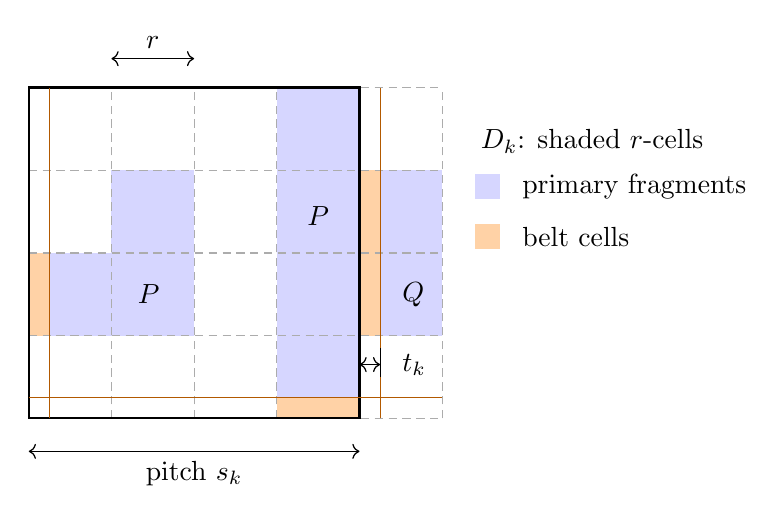
\begin{tikzpicture}[scale=1.05, line width=.45pt]
 \foreach \x/\y in {0/1,1/1,1/2,3/0,3/1,3/2,3/3,4/1,4/2}
   {\fill[blue!16] (\x,\y) rectangle +(1,1);}
 \fill[orange!35] (0,1) rectangle (.25,2);
 \fill[orange!35] (3,0) rectangle (4,.25);
 \fill[orange!35] (4,1) rectangle (4.25,3);
 \draw[step=1,gray!65,densely dashed] (0,0) grid (5,4);
 \draw[thick] (0,0) rectangle (4,4);
 \draw[orange!70!black] (.25,0)--(.25,4)
                          (4.25,0)--(4.25,4)
                          (0,.25)--(5,.25);
 \node at (1.45,1.5) {$P$};
 \node at (3.5,2.45) {$P$};
 \node at (4.65,1.5) {$Q$};
 \node[anchor=west] at (5.35,3.35) {$D_k$: shaded $r$-cells};
 \fill[blue!16] (5.4,2.65) rectangle (5.7,2.95);
 \node[anchor=west] at (5.85,2.8) {primary fragments};
 \fill[orange!35] (5.4,2.05) rectangle (5.7,2.35);
 \node[anchor=west] at (5.85,2.2) {belt cells};
 \draw[<->] (0,-.4)--(4,-.4);
 \node[below] at (2,-.4) {pitch $s_k$};
 \draw[<->] (1,4.35)--(2,4.35);
 \node[above] at (1.5,4.35) {$r$};
 \draw[<->] (4,.65)--(4.25,.65);
 \draw (4,.5)--(4,.85) (4.25,.5)--(4.25,.85);
 \node[anchor=west] at (4.4,.65) {$t_k$};
\end{tikzpicture}
\caption{A schematic portion of one ambient layer, not to scale.
Dashed lines mark the $r$-cells.  The thick square is one pitch cell;
its interior after removing the belt strips has side $s_k-t_k$.
All blue fragments in that interior share the primary identifier $P$,
even when disconnected.  The neighboring fragment has identifier $Q$.
Both primaries have family label $k\bmod2$; the orange belt cells are
filled and labeled in the next step.  The drawing concerns the ambient
layer $D_k$, before intersection with the physical set $A$.}
\label{geometry:layer-picture}
\end{figure}

\subsection{Filling the belts}

The remaining construction colors the belt cells while making every
positive-length interface between different tile identifiers join
opposite labels.  Point contacts will be dealt with separately.

Adjacent layer fine meshes have side ratio either 1 or 2.  They have a
common translated dyadic origin, including after the pitch shifts, which
were by multiples of their fine-cell sides.  Divide a side of a belt
cell at any corner of an opposing cell.  A larger side can be divided
only at its midpoint.  Along each resulting elementary segment, the
opposing region is either one primary or dummy tile, or one elementary
segment of another belt cell.  A layer boundary cannot change in the
interior of such a segment: layer edges lie on the coarser dyadic grids.

Join the center of each belt cell to the endpoints of its elementary
segments.  This makes a fan of at most eight triangles, with edges of
slopes $0,\infty,1,-1$.  A triangle facing a primary or dummy tile receives
the opposite label.  On a segment shared by two belt cells, assign any
opposite pair of labels to its two incident triangles, consistently on
both sides.  Within each belt cell merge each cyclic run of consecutive
triangles with the same label into one tile identifier.  Distinct runs
remain distinct identifiers; if all labels agree, the whole cell is one
tile.

Every positive-length interface between distinct identifiers now joins
opposite labels.  Across a cell side this follows from the assignment;
inside a fan it follows from merging equal-label neighbors.  Primaries
were already separated in the same layer, and adjacent-layer primaries
have opposite labels.  Thus a same-label contact between distinct tiles
can only be a point, and every such contact involves a belt cell.

Mark the center, the four corners, and the four side midpoints of every
belt cell.  Some midpoint marks are unnecessary for its fan, but adding
them simplifies the recursion.  Deduplicate coincident marks, assigning
a mark $v$ the scale $S_v$ equal to the smallest side length of a belt
cell that marked it.  There are at most nine times as many initial marks
as belt cells.

\begin{lemma}[Isolated stars of the initial mesh]
\label{geometry:initial-stars}
There is an absolute constant $a_0>0$, independent of the layer and the
chosen shifts, such that, on taking $k_0$ sufficiently large:
\begin{enumerate}
\item
Distinct marks $v,w$ satisfy
$\norm{v-w}_\infty\ge a_0\max(S_v,S_w)$.
\item
In the square $v+[-a_0S_v,a_0S_v]^2$, all active boundaries are straight
rays from $v$ in the eight axis and diagonal directions.  Each sector
between consecutive active rays has one tile identifier, and consecutive
sectors have opposite labels.  If there is no active ray, the square is
in one tile.
\end{enumerate}
An active boundary here means an interface of distinct identifiers;
seams removed by a merge are not boundaries.
\end{lemma}

\begin{proof}
Consider a belt cell of side $t=t_k$.  In its $10t$-neighborhood only its
own and adjacent layers can occur, by \eqref{geometry:nonadjacent} and
$t_k/2^k\to0$.  All fine-cell sides there are $t/2,t$, or $2t$.
Cell corners, fan centers, and side midpoints therefore lie on the affine
mesh $o+(t/4)\Z^2$.  All active lines have one of the four allowed slopes
and intercepts on this mesh.  Marks have local scales comparable to $t$.
Distinct marks have distance at least $t/4$, and a supporting line that
does not contain a given mark is at sup distance at least $t/8$ from it.
The same bounds apply to the nearest other endpoint of an incident
segment.
Choosing $a_0$ small gives both assertions locally.  Apply this argument
at the larger scale for a pair of nearby marks; pairs outside the local
neighborhood already satisfy the asserted separation.

The preceding coloring shows that two sectors separated by an active
ray have opposite labels.  Coincident boundary segments or inactive seams
are counted only once, so this describes the actual tile regions near
the mark.
\end{proof}

\subsection{Removing point contacts at successively smaller scales}

The purpose of the next construction is to make the birth template of
each newly created tile avoid the final actual sets of earlier tiles of
the same label.  Removing points only from the new tile would not provide
that property.  We remove a square from every old identifier incident
with the mark before creating its replacement.

Choose a fixed stopping scale $S_*$ sufficiently large that, for every
$S\ge S_*$, the dyadic halfside
\begin{equation}
\label{geometry:trim-radius}
 d(S)=2^{\lfloor\rho_0\log_2 S\rfloor}
\end{equation}
satisfies
\begin{equation}
\label{geometry:trim-margins}
 \tfrac12S^{\rho_0}\le d(S)\le S^{\rho_0},\qquad
 d(S)\le\frac{a_0}{1000}S.
\end{equation}
We will increase $S_*$ later to accommodate the collar estimate.  Choose
$k_0$ so that all initial mark scales are at least $S_*$.  At each
generation perform the following operations simultaneously at every
active mark $(v,S)$:
\begin{enumerate}
\item
Remove the closed square
$Q_v=v+[-d(S),d(S)]^2$ from every old tile identifier.
\item
If $d(S)<S_*$, leave its interior unassigned and declare it a terminal
exceptional square.
\item
Otherwise, continue the incident active rays through the square to its
center.  In each resulting sector give the new region the label opposite
to that of the corresponding exterior sector, with a new identifier for
each sector.  If there are no rays, use one opposite-label square.  Mark
the center, corners, and side midpoints of $Q_v$, all at scale $d(S)$,
for the next generation.
\end{enumerate}
A sector with angle exceeding $\pi$ need not be convex; it is a union of
at most eight of the triangles from the center to side corners and
midpoints.  Thus all replacement birth regions retain the required
finite description.  Every old ray meets the square perimeter at a
corner or side midpoint.  Figure~\ref{geometry:repair-picture} illustrates
the label reversal and the marks used at the next generation.

\begin{figure}[H]
\centering
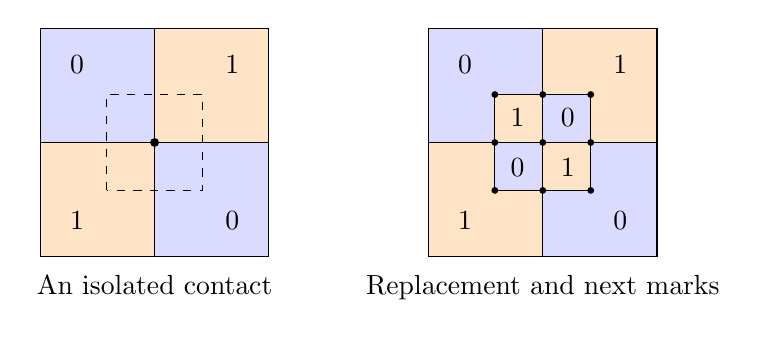
\begin{tikzpicture}[scale=1.45, line width=.45pt]
 \begin{scope}[xshift=-1.7cm]
  \fill[blue!14] (-1,0) rectangle (0,1);
  \fill[orange!22] (0,0) rectangle (1,1);
  \fill[blue!14] (0,-1) rectangle (1,0);
  \fill[orange!22] (-1,-1) rectangle (0,0);
  \draw (-1,-1) rectangle (1,1);
  \draw (-1,0)--(1,0) (0,-1)--(0,1);
  \draw[dashed] (-.42,-.42) rectangle (.42,.42);
  \node at (-.68,.68) {$0$}; \node at (.68,.68) {$1$};
  \node at (.68,-.68) {$0$}; \node at (-.68,-.68) {$1$};
  \fill (0,0) circle (1.1pt);
  \node[below] at (0,-1.08) {An isolated contact};
 \end{scope}
 \begin{scope}[xshift=1.7cm]
  \fill[blue!14] (-1,0) rectangle (0,1);
  \fill[orange!22] (0,0) rectangle (1,1);
  \fill[blue!14] (0,-1) rectangle (1,0);
  \fill[orange!22] (-1,-1) rectangle (0,0);
  \fill[orange!22] (-.42,0) rectangle (0,.42);
  \fill[blue!14] (0,0) rectangle (.42,.42);
  \fill[orange!22] (0,-.42) rectangle (.42,0);
  \fill[blue!14] (-.42,-.42) rectangle (0,0);
  \draw (-1,-1) rectangle (1,1);
  \draw (-1,0)--(1,0) (0,-1)--(0,1);
  \draw (-.42,-.42) rectangle (.42,.42);
  \node at (-.68,.68) {$0$}; \node at (.68,.68) {$1$};
  \node at (.68,-.68) {$0$}; \node at (-.68,-.68) {$1$};
  \node at (-.22,.22) {$1$}; \node at (.22,.22) {$0$};
  \node at (.22,-.22) {$1$}; \node at (-.22,-.22) {$0$};
  \foreach \x in {-.42,0,.42}
   \foreach \y in {-.42,0,.42}
    {\fill (\x,\y) circle (.85pt);}
  \node[below] at (0,-1.08) {Replacement and next marks};
 \end{scope}
\end{tikzpicture}
\caption{A four-sector example of the repair.  The square around the
contact is removed from every old tile, and its new sectors receive the
opposite labels.  Positive-length interfaces still join opposite labels.
Any same-label contacts involving the new tiles occur among the nine
marked points; the next, smaller removal separates them.  The proof also
allows any configuration of the eight permitted ray directions with
opposite labels in consecutive sectors.}
\label{geometry:repair-picture}
\end{figure}

We now verify that this procedure continues with uniform geometric
constants.  In particular, neither the separation constant nor the
isolation radius is allowed to deteriorate with the number of
generations.

\begin{lemma}[Uniform repair induction]
\label{geometry:repair-induction}
For a sufficiently small fixed choice of $a_0$ and the corresponding
threshold $S_*$, every active mark $(v,S)$ at every generation has a
terminal-square-free isolated star
$v+[-a_0S,a_0S]^2$ with the properties of
Lemma~\ref{geometry:initial-stars}.  Distinct active marks satisfy the same
separation inequality.  The simultaneous removal squares are disjoint.
Each replacement has opposite labels across every positive-length
interface of distinct identifiers, and its same-label contacts with old
remnants or peer replacements occur only at marks of the next generation.
Every descendant mark and every descendant birth region of a mark
$(v,S)$ lies within sup distance $2d(S)$ of $v$.  Each branch terminates
after finitely many generations.
\end{lemma}

\begin{proof}
Suppose the assertions hold at one generation.  By
\eqref{geometry:trim-margins}, the squares of radius $6d(S)$ are contained
in their parent stars.  They are also disjoint from all other current
removal squares.  Indeed for parent marks $(v,S),(w,T)$,
\[
 \norm{v-w}_\infty\ge a_0\max(S,T),\qquad
 6d(S)+d(T)\le \frac{7a_0}{1000}\max(S,T).
\]
Thus each modification sees only its parent's radial boundaries.

Across a new perimeter segment away from ray hits, the new interior
label was chosen opposite to the exterior label.  Across an interior
ray, the two labels remain opposite because the two exterior labels were
opposite.  All other positive-length interfaces are unchanged.  Contacts
not lying in the relative interior of one of these segments are among
the center, corners, or side midpoints of the new square.  This proves the
coloring and contact assertions.

Normalize one removal square to $[-1,1]^2$.  Its post-replacement
boundaries are subsets of the original eight radial rays together with
the four lines supporting this square.  The possible new marks are the
nine points of $\{-1,0,1\}^2$.  Every nonincident supporting line stays at
a fixed positive distance from a mark, and every other endpoint stays
at distance at least one.  Thus a fixed sufficiently small $a_0$ gives
an isolated radial star at each child, on the child's scale $d(S)$.
This is the same finite line configuration at every generation, so no
iteration of a shrinking constant is involved.

Two children of the same parent are at least $d(S)$ apart.  For children
of different parents their separation is at least
\[
 a_0\max(S,T)-d(S)-d(T)
 \ge \frac{a_0}{2}\max(S,T),
\]
which is larger than $a_0\max(d(S),d(T))$ by
\eqref{geometry:trim-margins}.  Their isolated-star squares therefore
satisfy the original separation invariant as well.

The child stars lie inside the parent star.  Consequently they avoid
all terminal squares from earlier generations.  A terminal square
created at another parent in the current generation is excluded by the
same cross-parent distance estimate.  For a direct statement covering
all later generations, each successive child displacement is at most
the preceding removal radius, and subsequent radii shrink by the fixed
factor at most $a_0/1000$.  Their sum, including the radius of the final descendant birth square,
is less than $2d(S)$.  Subtrees of distinct parents are therefore
separated by the preceding inequalities,
even if one subtree has already terminated.  This proves the asserted
terminal-square avoidance and descendant bound.

Finally, as long as a branch continues, its successive scales satisfy
$S_{j+1}=d(S_j)\le S_j^{\rho_0}$ with $\rho_0<1$.  After finitely many
steps the computed next halfside is below $S_*$, and that removal is
terminal.  This
completes the induction.
\end{proof}

All geometric edges avoid lattice sites.  Initially their vertices are
in $o+\Z^2$ because $r,s_k,t_k$ are dyadic integers, and the halfsizes and
midpoints used are integral.  In the recursion each new center, corner,
and midpoint is obtained by adding an integer vector to the preceding
center; the halfside $d(S)$ is an integer.  Enlarge $S_*$ once so that a
terminal halfside produced from $S\ge S_*$ is still at least two.
Every supporting line consequently has equation
\[
 x_1=o_1+m,\quad x_2=o_2+m,\quad
 x_1+x_2=o_1+o_2+m,\quad\text{or}\quad
 x_1-x_2=o_1-o_2+m,\qquad m\in\Z.
\]
None contains a point of $\Z^2$.  We may therefore use open actual tile
regions and closed birth regions without any convention for assigning a
lattice site on an interface.  The final open tile regions, the unaltered
part of the dummy region, and terminal-square interiors partition all
lattice sites.

\subsection{Separation from earlier actual regions}

Order tile identifiers as follows: all primaries first, all initial belt
tiles second, and then the replacement tiles by their generation of
birth.  Ties within each class can be broken arbitrarily.  The dummy tile
is excluded from this order.  Primaries already have the required
same-label separation from other primaries.  The next lemma handles all
remaining identifiers and explains why the order uses actual earlier
regions.

\begin{lemma}[Birth-template separation]
\label{geometry:birth-separation}
There is a fixed $c_1>0$ such that the following holds.  Let $\mathcal B$
be the closed birth region of an initial belt tile of side scale $u=t_k$,
or of a replacement tile whose removal square has halfside $u$.
Then its distance from the final actual region of every earlier or peer
identifier of the same label is at least $c_1u^{\rho_0}$.  A peer means
another initial belt tile, or another replacement born at the same
generation, respectively.
\end{lemma}

\begin{proof}
At the birth of an initial belt tile, compare its closure with the
primary and belt closures at that time.  At the birth of a replacement,
compare it with the old remnants \emph{after} that generation's removal
squares have been cut out, and with the peer replacements.  Each final
actual region is a subset of the corresponding compared region.  In
particular an ancestor is compared after its square has been removed;
its original birth region need not be disjoint from the new one.

Restrict attention to a closed box obtained by enlarging the tile's cell
or removal square by $2u$ in each direction.  Points outside this box are
at distance at least $2u$ from the birth region.  Translate by its cell
corner, or by its removal center, and rescale lengths by $u$.  Only
finitely many local pairs of closed regions can arise:
\begin{itemize}
\item
For belts, the nearby active lines and endpoints lie on the affine
quarter mesh, with their four prescribed slopes.  In a bounded box there
are only finitely many such lines and endpoints.  The local closures are
unions of faces of their arrangement; allowing all possible identifier
groupings still leaves only finitely many pairs of unions.  We classify
only the restrictions to this box: disconnected pieces of an identifier
outside it do not change the local pattern.
\item
For a replacement, the enlarged box lies in the isolated star of its
parent, by \eqref{geometry:trim-margins}.  It sees only the old radial
layout and the new square and sectors.  These lie on a fixed finite
arrangement in the rescaled coordinates.  Other parents' simultaneous
modifications do not enter this box.
\end{itemize}
Thus there is a common positive scale for the isolation neighborhoods
used in all these comparisons.

The two compared closures of the same label have no positive-length
interface.  Their intersections, if any, are contact marks by the belt
construction or Lemma~\ref{geometry:repair-induction}.  At a belt contact
the mark scale is comparable with $u$ (neighboring belt scales differ by
at most two); at a replacement contact it is $u$.  Choose disjoint open
contact squares of radius $\lambda u$ inside the isolated stars, for a
fixed sufficiently small $\lambda>0$.

First consider pairs of points $(x,y)$ in the two compared closures that
do not both belong to the same open contact square.  This condition
specifies a closed subset of the compact product of the two local
closures.  On it the distance $\norm{x-y}_\infty$ has a positive minimum:
if the minimum were zero, $x=y$ would be a common contact, and both points
would belong to its open contact square.  Since the list of rescaled
patterns is finite, the minimum is uniformly at least $c_2u$ whenever
this subset is nonempty.

It remains to consider $x,y$ in one contact star centered at $v$.
Inside that star each closure is a union of closed radial sectors.
Their direction sets are disjoint.  A shared direction would give a
shared ray segment, contrary to the absence of positive-length
same-label contacts.  Their boundary directions are among the eight
axis and diagonal directions, so the angle between their direction sets
is at least $\pi/4$.  Elementary Euclidean geometry, followed by
comparison of Euclidean and sup norms, gives
\begin{equation}
\label{geometry:angular-gap}
 \norm{x-y}_\infty
 \ge c_3\max\{\norm{x-v}_\infty,\norm{y-v}_\infty\}.
\end{equation}
For example, the squared Euclidean distance between radial vectors of
lengths $a,b$ and angle $\theta\ge\pi/4$ is
$(a-b)^2+2ab(1-\cos\theta)$, which bounds a fixed multiple of
$\max(a,b)^2$.

At the immediately following trim, the compared old or peer identifier
loses a square about $v$ of radius at least $c_4u^{\rho_0}$, by
\eqref{geometry:trim-radius} and comparability of mark scales.  This
removal also occurs if the square is terminal.  That identifier only
shrinks afterward.  Thus a point $y$ in its final actual region has
$\norm{y-v}_\infty\ge c_4u^{\rho_0}$, and
\eqref{geometry:angular-gap} supplies the required lower bound for pairs
inside the contact star.  Together with the preceding compactness
estimate and the exterior-of-box estimate this proves the lemma.
\end{proof}

The lemma compares the entire new birth region with an older actual
region.  Later deletions from the new tile are irrelevant to this
estimate.  This is the form needed for applying the collar estimate to
its untrimmed template and then discarding part of that template.

\subsection{Counting exceptional sites and verifying the templates}

Let an initial mark have scale $S$.  Along a branch,
$\log S_j\le\rho_0^j\log S$ until termination.  Its depth is therefore at
most
\[
 C+C\log\log(e^e+S).
\]
There are at most nine children per mark.  Consequently the number of
marks and replacements descended from this initial mark is at most
\begin{equation}
\label{geometry:descendant-count}
 C\bigl(\log(S+2)\bigr)^{C}.
\end{equation}
The constants are fixed; their magnitude is immaterial for a
size-independent area bound.  The scale of a mark initially belonging to
layer $k$ is comparable with $t_k$, and hence its logarithm is at most
$C(k+1)$.  By \eqref{geometry:belt-count}, the total number of belt tiles,
marks, and replacements is bounded by
\begin{equation}
\label{geometry:total-repairs}
 Cb\sum_{k\ge k_0}2^{-k\delta_0/2}(k+1)^C\le C'b.
\end{equation}
In particular this total is finite, even before restricting the
construction to the finite domain.

Each terminal square has halfside below the fixed $S_*$ and therefore
contains at most $C S_*^2$ lattice sites.  The dummy region has at most
$C|Z|$ cells of the fixed side $2^{k_0}$ and hence at most $Cb$ lattice
sites.  Let $D$ be the sites of $A$ that remain in the dummy identifier or
lie in terminal squares.  Sites overwritten by a replacement are no
longer counted as dummy sites.  Equations~\eqref{geometry:descendant-count}
and \eqref{geometry:total-repairs} give
\begin{equation}
\label{geometry:bad-sites}
 |D|\le Cb.
\end{equation}
This counts ambient sites and then intersects with $A$.  Missing sites,
holes, thin parts, and disconnected components of $\Lambda$ can only
reduce the count.

We now assign scanner scales to the birth templates.  Let
$T=\mathcal B\cap\Z^2$ for a birth region $\mathcal B$.
For a primary in layer $k$, take
\begin{equation}
\label{geometry:primary-scale}
 s_0=r=2^k,\qquad n=\left\lceil C_P r^{1+2\delta_0}\right\rceil.
\end{equation}
By \eqref{geometry:primary-pieces}, it has at most
$N_0\le C(s_k/r+2)^2\le C r^{2\delta_0}$ rectangular pieces, each of
sup-norm diameter at most $s_0$.  Choosing $C_P$ large ensures
\[
 n\ge C_{\mathrm{tpl}}N_0(s_0+1),\qquad
 \diam_\infty T\le s_k\le n.
\]
The birth template has endpoint distance at least $C_0r$, so the safe
clearance in Definition~\ref{scanner:template} follows from the choice
of $C_0$.  The exponent inequalities give, uniformly over primaries,
\begin{equation}
\label{geometry:primary-limits}
 L=\lfloor n^{1-\ell}\rfloor=o(r),\qquad
 n^\beta=o(t_k),\qquad n^\beta=o(r).
\end{equation}

For a belt tile take $u=t_k$, $s_0=u$, and
$n=\lceil C_Bu\rceil$.  It is a union of at most eight of the closed fan
triangles.  For a replacement whose removal halfside is $u$, take
$s_0=2u$ and $n=\lceil C_Bu\rceil$.  Subdivision into the triangles from
the center to corners and midpoints again uses at most eight pieces,
including for a wide sector or a homogeneous square.  Choose $C_B$ large
enough for all of these templates to satisfy
$n\ge C_{\mathrm{tpl}}N_0(s_0+1)$ and $\diam_\infty T\le n$.
In both cases $L=o(u)$.

Their cut clearance remains much larger than their size.  An initial
belt cell in $D_k$ has endpoint distance at least $C_0r$.
A mark on its closure has the same lower bound.  By
Lemma~\ref{geometry:repair-induction}, every descendant lies within
$2d(S)\le2t_k^{\rho_0}=o(t_k)$ of that mark.  After increasing $k_0$, all
its descendant birth templates therefore have endpoint distance at least
$(C_0-1)r$.  This also covers replacements extending into the dummy
region.  Since their side scales are at most $2t_k=o(r)$, their endpoint
distance exceeds both $4D_0s_0$ and $2n^\beta$.

These checks establish the exact geometric hypotheses of
Lemma~\ref{scanner:templates}.  In particular, for every birth template,
its dilated layers up to $L$ have the stipulated row and perimeter
bounds, and the safe-box estimate yields the core and shell entropy
bounds needed by Proposition~\ref{prop:collar}.  The verification uses
the finite union of convex pieces; no assertion that a primary, a sector
run, or its intersection with $A$ is a rectangle is needed.

For clarity, the relevant thresholds can be fixed in the following
order.  First fix $C_0,C_P,C_B$ and the absolute isolation constant.
Next increase $S_*$ until \eqref{geometry:trim-margins} holds, all belt and
replacement scanner scales are at least $n_*$, and
\begin{equation}
\label{geometry:fine-clearance}
 c_1u^{\rho_0}>2\lceil C_Bu\rceil^\beta
 \qquad(u\ge S_*).
\end{equation}
This is possible because $\rho_0>\beta$.  Finally increase $k_0$ to
ensure that initial belt scales exceed $S_*$, that all primary scales
exceed $n_*$, and that all the uniform large-scale inequalities just used
hold.  For primaries this includes their same-layer gap
$t_k>2n^\beta$, their nonadjacent-layer gaps, and
\eqref{geometry:primary-limits}.  Floors and ceilings only change fixed
multiplicative constants.

We can now finish the geometric proposition.  Retain just identifiers
whose final actual regions meet $A$, and let $X_i$ be those intersections,
ordered as above.  There are finitely many, since these nonempty sets
are pairwise disjoint subsets of a finite set.  They partition $A\setminus
D$, and each lies in its birth template.  Equations
\eqref{geometry:layer-distance}, \eqref{geometry:primary-limits}, and the
descendant clearance prove \eqref{geometry:cut-clearance}.
For primaries, earlier same-label primaries are separated by $t_k$ in the
same layer or by \eqref{geometry:nonadjacent} in other layers.  For belts
and replacements, Lemma~\ref{geometry:birth-separation} and
\eqref{geometry:fine-clearance} prove
\eqref{geometry:ordered-clearance}.  Restricting an older actual region
to $A$ preserves these lower bounds.

There are at most $Cb$ primaries per layer, and their scales satisfy
$n\ge c2^{(1+2\delta_0)k}$.  Their error sum is therefore bounded by
\[
 Cb\sum_{k\ge k_0}2^{-100(1+2\delta_0)k}\le C'b.
\]
The total number of other tiles is $O(b)$ by
\eqref{geometry:total-repairs}, and each has $n\ge1$.  Their error sum is
also $O(b)$.  This proves every assertion of
Proposition~\ref{prop:two-families}.

\subsection{Proof of the area law}

\begin{proof}[Proof of Theorem~\ref{thm:area}]
The empty domain and the empty or full region have zero entropy.
Put $b=|\partial_\Lambda A|$. If $b=0$,
Lemma~\ref{lem:zero-boundary} gives $S_\Omega(A)=0$.

Assume $b>0$.  Choose $n_*$ large enough for
Proposition~\ref{prop:collar} and Proposition~\ref{prop:amplification}
with $M=100$ to apply to the templates of
Proposition~\ref{prop:two-families}, uniformly with the stated template
bounds.  Increase it so that every radius $r$ supplied by amplification
at scale $n\ge n_*$ satisfies $L+2r<n^\beta$.  Let $D,X_i,T_i,n_i,f_i$ be the
resulting geometric decomposition, and put
\[
 S_i=A\cap\bigl(T_i+[-L_i,L_i]^2_{\Z}\bigr),\qquad
 J_i=(\Lambda\setminus A)\cup
       \bigcup_{\substack{j<i\\f_j=f_i}}X_j.
\]
Here $[-L_i,L_i]^2_{\Z}$ denotes the integer square.  For each $i$, let
$r_i$ be the radius supplied by amplification, using the size, boundary,
and information bounds from Proposition~\ref{prop:collar}.  The resulting
mutual-information estimate applies to $A\cap T_i$ against any sites
outside the graph neighborhood $N_{2r_i}^{\Lambda}(S_i)$.

We verify this condition for the whole set $J_i$, rather than for its
individual pieces.  A graph path of length at most $2r_i$ from $S_i$
stays within ambient distance $L_i+2r_i<n_i^\beta$ of $T_i$.
Equation~\eqref{geometry:ordered-clearance} excludes every earlier
same-family $X_j$ jointly.  Such a path also cannot reach
$\Lambda\setminus A$: its first crossing of the cut would put an endpoint
of a cut edge within that ambient distance of $T_i$, contradicting
\eqref{geometry:cut-clearance}.  Thus
\[
 J_i\subseteq\Lambda\setminus N_{2r_i}^{\Lambda}(S_i).
\]
Proposition~\ref{prop:amplification} and monotonicity under discarding
part of its first system yield
\[
 I_\Omega(X_i:J_i)
 \le I_\Omega(A\cap T_i:J_i)\le C n_i^{-100}.
\]
These estimates all concern the same original state $\Omega$, although
the auxiliary construction used to prove each estimate may differ.

Apply Lemma~\ref{geometry:cancellation} to the two labels.  Since each
site has dimension $q$,
\[
 S_\Omega(A)
 \le |D|\log q+\frac C2\sum_i n_i^{-100}
 \le C' b.
\]
Every choice of threshold and every constant in this proof depends only
on the fixed local dimension, interaction range and norm bound, and
spectral gap.  None depends on the size, shape, connectedness, or holes
of $\Lambda$, or on the choice of $A$.  This proves the theorem.
\end{proof}

\begingroup
\small
\bibliographystyle{plain}
\bibliography{references}
\endgroup
\end{document}
